% Original Source: http://mitschriebwiki.nomeata.de/data/WS10/Ana3Bachelor.tex
\documentclass[a4paper,oneside,DIV15,BCOR12mm]{scrbook}
\usepackage{mathe}
\usepackage{saetze-schmoeger}

\lecturer{Dr. C. Schmoeger}
\semester{Wintersemeseter 10/11 und 12/13}
\scriptstate{complete}

\author{Die Mitarbeiter von \href{http://mitschriebwiki.nomeata.de/}{mitschriebwiki.nomeata.de} 
und \href{https://github.com/MartinThoma/LaTeX-examples/tree/master/documents}{GitHub}}
\title{Analysis III - Bachelorversion}
\makeindex

\hypersetup{ 
  pdfauthor   = {Die Mitarbeiter von mitschriebwiki.nomeata.de und GitHub}, 
  pdfkeywords = {Analysis}, 
  pdftitle    = {Analysis III} 
} 

\begin{document}
\maketitle

\renewcommand{\thechapter}{\Roman{chapter}}
%\chapter{Inhaltsverzeichnis}
\addcontentsline{toc}{chapter}{Inhaltsverzeichnis}
\tableofcontents

\chapter*{Vorwort}

\section*{Über dieses Skriptum}
Dies ist ein Mitschrieb der Vorlesung \glqq Analysis III\grqq\ von 
Herrn Schmoeger im Wintersemester 2010 an der Universität Karlsruhe 
(KIT). Die Mitschriebe der Vorlesung werden mit ausdrücklicher 
Genehmigung von Herrn Schmoeger hier veröffentlicht, Herr Schmoeger 
ist für den Inhalt nicht verantwortlich.

\section*{Wer}
Gestartet wurde das Projekt von Joachim Breitner. Beteiligt an diesem
Mitschrieb sind Rebecca Schwerdt, Philipp Ost, Jan Ihrens, Peter Pan
und Benjamin Unger.

Im September 2012 wurde das Skript mit der Revisionsnummer 7132 von
mitschriebwiki auf \href{https://github.com/MartinThoma/LaTeX-examples/blob/master/documents/Analysis%20III}{GitHub} hochgeladen.

\section*{Wo}
Alle Kapitel inklusive \LaTeX-Quellen können unter 
\href{http://mitschriebwiki.nomeata.de}{mitschriebwiki.nomeata.de} 
abgerufen werden.
Dort ist ein \emph{Wiki} eingerichtet und von Joachim Breitner um die 
\LaTeX-Funktionen erweitert.
Das heißt, jeder kann Fehler nachbessern und sich an der Entwicklung
beteiligen. Auf Wunsch ist auch ein Zugang über \emph{Subversion} 
möglich.

Oder man geht auf \href{https://github.com/MartinThoma/LaTeX-examples/blob/master/documents/Analysis%20III/}{github},
erstellt einen Fork und kann direkt Änderungen umsetzen.


\renewcommand{\thechapter}{\arabic{chapter}}
\renewcommand{\chaptername}{§}
\renewcommand*{\chapterformat}{§\,\thechapter \enskip}
\setcounter{chapter}{-1}

\chapter{Vorbereitungen}
\label{Kapitel 0}

In diesem Paragraphen seien $X,Y,Z$ Mengen ($\ne\emptyset$) und 
$f: X\to Y,\; g:Y\to Z$ Abbildungen.

\begin{enumerate}
    \index{Potenzmenge}
    \index{Disjunktheit}
    \item 
    \begin{enumerate}
        \item $\mathcal{P}(X):=\{A:A\subseteq X\}$ heißt 
              \textbf{Potenzmenge} von $X$.
        \item Sei $\fm\subseteq\mathcal{P}(X)$, so heißt $\fm$ 
              \textbf{disjunkt}, genau dann wenn $A\cap B=\emptyset$ 
              für $A,B\in\fm$ mit $A\ne B$.
        \item Sei $(A_j)$ eine Folge in $\mathcal{P}(X)$ (also 
              $A_j\subseteq X$), so heißt $(A_j)$ \textbf{disjunkt},
              genau dann wenn $\{A_1,A_2,\dots\}$ disjunkt ist.\\
              \textbf{Schreibweise}:\\
              \begin{align*}
                \dot{\bigcup}_{j=1}^\infty &:=\bigcup_{j=1}^\infty A_j\\
                \bigcup_{j=1}^\infty A_j   &:=\bigcup A_j\\
                \bigcap_{j=1}^\infty A_j   &:=\bigcap A_j\\
                \sum_{j=1}^\infty a_j      &=: \sum a_j
              \end{align*}
    \end{enumerate}
    \item Sei $A\subseteq X$, $\mathds{1}_A : X \rightarrow R$ 
          definiert durch:
          \[\mathds{1}_A(x):= \begin{cases}
                1 &\text{falls } x\in A\\
                0 &\text{falls } x\in A^c
            \end{cases}\]
          wobei $A^c:=X\setminus A$. $\mathds{1}_A$ heißt die
          \textbf{charakteristische Funktion} oder 
          \textbf{Indikatorfunktion von A}.
    \item Sei $B\subseteq Y$ dann ist $f^{-1}(B):=\{x\in X: f(x)\in B\}$ 
          und es gelten folgende Eigenschaften:
          \begin{enumerate}
            \item $f^{-1}(B^c)=f^{-1}(B)^c$
            \item Ist $B_j$ eine Folge in $\mathcal{P}(Y)$, so gilt:
                  \begin{align*}
                  f^{-1}(\bigcup B_j)=\bigcup f^{-1}(B_j)\\
                  f^{-1}(\bigcap B_j)=\bigcap f^{-1}(B_j)\\
                  \end{align*}
            \item Ist $C\subseteq Z$, so gilt:
                  \[(g\circ f)^{-1}(C)=f^{-1}(g^{-1}(C))\]
          \end{enumerate}
\end{enumerate}

\begin{definition}
    \index{offen}
    Sei $n \in \mdn$ und $\emptyset \neq X \subseteq \mdr^n$ und 
    $A \subseteq X$.

    $A$ heißt $\stackrel{\text{offen}}{\text{abgeschlossen}}$ in 
    $X :\Leftrightarrow \exists B \subseteq \mdr^n$. 
    $B$ ist $\stackrel{\text{offen}}{\text{abgeschlossen}}$ und 
    $A = B \cap X$
\end{definition}

\begin{satz}
    Sei $\emptyset \neq X \subseteq \mdr^n \; A \subseteq X$ und
    $f: X \rightarrow \mdr^n$.

    \begin{enumerate}
        \item $A$ ist offen in $X \Leftrightarrow \forall x \in A$ 
              ex. eine Umgebung $U$ von $x$ mit $U \cap X \subseteq A$
        \item $A$ ist abgeschlossen in $X$\\
              $\Leftrightarrow X \setminus A$ ist offen in $X$\\
              $\Leftrightarrow$ für jede konvergente Folge $(a_k)$ 
              in $A$ mit $\lim a_k \in X$ ist $\lim a_k \in A$
        \item Die folgenden Aussagen sind äquivalent:
              \begin{enumerate}
                \item $f \in C(X, \mdr^m)$
                \item für jede offene Menge $B \subseteq \mdr^m$ ist 
                      $f^{-1}(B)$ offen in $X$
                \item für jede abgeschlossene Menge $B \subseteq \mdr^m$ ist 
                      $f^{-1}(B)$ abgeschlossen in $X$
              \end{enumerate}
    \end{enumerate}
\end{satz}

\chapter{$\sigma$-Algebren und Maße}
\label{Kapitel 1}

In diesem Paragraphen sei $X \neq \emptyset$ eine Menge.

\begin{definition}
    \index{$\sigma$-!Algebra}
    Sei $\fa\subseteq\mathcal{P}(X)$, $\fa$ heißt eine 
    \textbf{$\sigma$-Algebra} auf $X$, wenn gilt:
    \begin{enumerate}
        \item[($\sigma_1$)] $X\in\fa$
        \item[($\sigma_2$)] Ist $A\in\fa$, so ist auch $A^c\in\fa$.
        \item[($\sigma_3$)] Ist $(A_j)$ eine Folge in $\fa$, so ist 
                            $\bigcup A_j\in\fa$.
    \end{enumerate}
\end{definition}

\begin{beispieleX}
    \begin{enumerate}
        \item $\Set{X,\emptyset}$ und $\mathcal{P}(X)$ sind 
              $\sigma$-Algebren auf $X$.
        \item Sei $A\subseteq X$, dann ist $\Set{X,\emptyset, A, A^c}$ 
              eine $\sigma$-Algebra auf $X$.
        \item $\fa:=\Set{A\subseteq X | A \text{ abzählbar oder } A^c \text{ abzählbar}}$ 
              ist eine $\sigma$-Algebra auf $X$.
    \end{enumerate}
\end{beispieleX}

\begin{lemma}
\label{Lemma 1.1}
Sei $\fa$ eine $\sigma$-Algebra auf $X$, dann:
\begin{enumerate}
\item $\emptyset\in\fa$
\item Ist $(A_j)$ eine Folge in $\fa$, so ist $\bigcap A_j\in\fa$.
\item Sind $A_1,\dots,A_n\in\fa$, so gilt:
\begin{enumerate}
\item $A_1\cup\cdots\cup A_n\in\fa$
\item $A_1\cap\cdots\cap A_n\in\fa$
\item $A_1\setminus A_2\in\fa$
\end{enumerate}
\end{enumerate}
\end{lemma}

\begin{beweis}
    \begin{enumerate}
    \item \folgtnach{$\sigma_2$} $\emptyset=X^c\in\fa$.
    \item $D:=\bigcap A_j$. $D^c=\bigcup A_j^c\in\fa$ (nach 
          ($\sigma_2$) und ($\sigma_3$)), also gilt auch 
          $D=(D^c)^c\in\fa$.
    \item \begin{enumerate}
            \item \folgtnach{($\sigma_3$) mit $A_{n+j}:=\emptyset$ ($j\ge 1$)} 
                  $A_1\cup\cdots\cup A_n\in\fa$.
            \item \folgtnach{(2) mit $A_{n+j}:=X$ ($j\ge 1)$} 
                  $A_1\cap\cdots\cap A_n\in\fa$.
            \item $A_1\setminus A_2=A_1\cap A_2^c\in\fa$
          \end{enumerate}
    \end{enumerate}
\end{beweis}

\begin{lemma}
    \label{Lemma 1.2}
    Sei $\cf \neq \emptyset$ eine Menge von $\sigma$-Algebren auf $X$. 
    Dann ist 
    \[\fa_0:=\bigcap_{\fa\in\cf}\fa\]
    eine $\sigma$-Algebra auf $X$.
\end{lemma}

\begin{beweis}
    \begin{enumerate}
        \item[($\sigma_1$)] $\forall\fa\in\cf:X\in\fa\implies X\in\fa_0$.
        \item[($\sigma_2$)] Sei $A\in\fa_0$, dann gilt:
          \begin{align*}
            \forall\fa\in\cf:A\in\fa &\implies \forall\fa\in\cf:A^c\in\fa\\
                                     &\implies A^c\in\fa_0
          \end{align*}
        \item[($\sigma_3$)] Sei $(A_j)$ eine Folge in $\fa_0$, dann 
            ist $(A_j)$ Folge in $\fa$ für alle $\fa\in\cf$, dann gilt:
          \begin{align*}
            \forall\fa\in\cf:\bigcap A_j\in\fa \implies \bigcap A_j\in\fa_0
          \end{align*}
    \end{enumerate}
\end{beweis}

\begin{definition}
    \index{Erzeuger}
    Sei $\emptyset \neq \mathcal{E} \subseteq \mathcal{P}(X)$ und 
    $\cf:=\{\fa:\fa$ ist $\sigma$-Algebra auf $X$ mit 
    $\mathcal{E}\subseteq\fa\}$. Definiere
    \[\sigma(\mathcal{E}):=\bigcap_{\fa\in\cf}\fa\]
    \folgtnach{1.2} $\sigma(\mathcal{E})$ ist eine $\sigma$-Algebra 
    auf $X$. $\sigma(\mathcal{E})$ heißt die 
    \textbf{von $\mathcal{E}$ erzeugte $\sigma$-Algebra}. 
    $\mathcal{E}$ heißt ein \textbf{Erzeuger} von 
    $\sigma(\mathcal{E})$.
\end{definition}

\begin{lemma}
    \label{Lemma 1.3}
    Sei $\emptyset\ne\mathcal{E}\subseteq\mathcal{P}(X)$.
    \begin{enumerate}
        \item $\mathcal{E}\subseteq\sigma(\mathcal{E})$. 
              $\sigma(\mathcal{E})$ ist die "`kleinste"' 
              $\sigma$-Algebra auf $X$, die $\mathcal{E}$ enthält.
        \item Ist $\mathcal{E}$ eine $\sigma$-Algebra, so ist 
              $\sigma(\mathcal{E})=\mathcal{E}$.
        \item Ist $\mathcal{E}\subseteq\mathcal{E}'$, so ist 
              $\sigma(\mathcal{E})\subseteq\sigma(\mathcal{E}')$.
    \end{enumerate}
\end{lemma}

\begin{beweis}
    \begin{enumerate}
        \item Klar nach Definition.
        \item $\fa:=\mathcal{E}$, dann gilt 
              $\fa\subseteq\sigma(\mathcal{E})\subseteq\fa$.
        \item $\mathcal{E}\subseteq\mathcal{E}'\subseteq\sigma(\mathcal{E}')$, 
              also folgt nach Definition 
              $\sigma(\mathcal{E})\subseteq\sigma(\mathcal{E}')$.
    \end{enumerate}
\end{beweis}

\begin{beispiel}
    \begin{enumerate}
        \item Sei $A\subseteq X$ und $\mathcal{E}:=\{A\}$. Dann ist 
              $\sigma(\mathcal{E})=\{X,\emptyset,A,A^c\}$.
        \item $X:=\{1,2,3,4,5\}, \mathcal{E}:=\{\{1\},\{1,2\}\}$. 
              Dann gilt:
              \[\sigma(\mathcal{E}):=\{X,\emptyset, \{1\},\{2\},\{1,2\},\{3,4,5\},\{1,3,4,5\},\{2,3,4,5\}\}\]
    \end{enumerate}
\end{beispiel}

\begin{erinnerung}
    \index{Offenheit}\index{Abgeschlossenheit}
    Sei $d\in\mdn, X\subseteq\mdr^d$. $A\subseteq X$ heißt 
    \textbf{offen} (\textbf{abgeschlossen}) in $X$, genau dann wenn 
    ein offenes (abgeschlossenes) $G\subseteq\mdr^d$ existiert mit 
    $A=X\cap G$.\\
    Beachte: $A$ abgeschlossen in $X$ $\iff$ $X\setminus A$ offen in 
    $X$.
\end{erinnerung}

\begin{definition}
    \index{Borel!$\sigma$-Algebra}\index{$\sigma$-!Algebra, Borelsche}
    \index{Borel!Mengen}
    Sei $X\subseteq\mdr^d$.
    \begin{enumerate}
        \item $\mathcal{O}(X):=\Set{A\subseteq X | A \text{ ist offen in } X}$
        \item $\fb(X):=\sigma(\mathcal{O}(X))$ heißt 
              \textbf{Borelsche $\sigma$-Algebra} auf $X$.
        \item $\fb_d:=\fb(\mdr^d)$. Die Elemente von $\fb_d$ heißen 
              \textbf{Borelsche Mengen} oder \textbf{Borel-Mengen}.
    \end{enumerate}
\end{definition}

\begin{beispiel}
    \begin{enumerate}
        \item Sei $\emptyset \neq X\subseteq\mdr^d$. Ist $A\subseteq$ 
              $\stackrel{\hbox{offen}}{\hbox{abgeschlossen}}$
              in $X$, so ist $A\in\fb(X)$.
        \item Ist $A\subseteq\mdr^d$ 
              $\stackrel{\hbox{offen}}{\hbox{abgeschlossen}}$,
              so ist $A\in\fb_d$.
        \item Sei $d=1, A=\mdq$. $\mdq$ ist abzählbar, also 
              $\mdq=\{r_1,r_2,\dots\}$ (mit $r_i\ne r_j$ für $i\ne j$). 
              Also ist $\mdq=\bigcup \{r_j\}$. Sei nun $r\in\mdq$, 
              dann ist $B:=(-\infty,r)\cup(r,\infty)\in\fb_1$. Daraus 
              folgt $\{r_j\}\in\fb_1$, also auch $\mdq\in\fb_1$.\\
              Allgemeiner lässt sich zeigen: 
              $\mdq^d:=\{(x_1,\dots,x_n):x_j\in\mdq (j=1,\dots,n)\}\in\fb_d$.
        \item Sei $x_0 \in \mdr^d, \Set{x_0}$ ist abgeschlossen
              $\Rightarrow \Set{x_0} \in \fb$
    \end{enumerate}
\end{beispiel}

\begin{definition}
    \index{Intervall}
    \index{Halbraum}
    \begin{enumerate}
    \item Seien $I_1,\dots,I_d$ Intervalle in $\mdr$. 
          $I_1\times\cdots\times I_d$ heißt ein \textbf{Intervall} 
          in $\mdr^d$.
    \item Seien $a=(a_1,\dots,a_d), b=(b_1,\dots,b_d)\in\mdr^d$.
          \[a\le b:\iff a_j\le b_j\quad (j=1,\dots,d)\]
    \item Seien $a,b\in\mdr^d$ und $a\le b$.
          \begin{align*}
            (a,b) &:= (a_1,b_1)\times\cdots\times(a_d,b_d)\\
            (a,b] &:= (a_1,b_1]\times\cdots\times(a_d,b_d]\\
            [a,b) &:= [a_1,b_1)\times\cdots\times[a_d,b_d)\\
            [a,b] &:= [a_1,b_1]\times\cdots\times[a_d,b_d]
        \end{align*}
        mit der Festlegung $(a,b):=(a,b]:=[a,b):=\emptyset$, falls 
        $a_j=b_j$ für ein $j\in\{1,\dots,d\}$.
    \item Für $k\in\{1,\dots,d\}$ und $\alpha\in\mdr$ definiere die 
          folgenden \textbf{Halbräume}:
          \begin{align*}
            H_k^-(\alpha) &:= \Set{(x_1,\dots,x_d)\in\mdr^d:x_k\le\alpha}\\
            H_k^+(\alpha) &:= \Set{(x_1,\dots,x_d)\in\mdr^d:x_k\ge\alpha}
          \end{align*}
    \end{enumerate}
\end{definition}

Beispiel für ein Intervall $(a_1, b_1) \times [a_2, b_2]$:\\
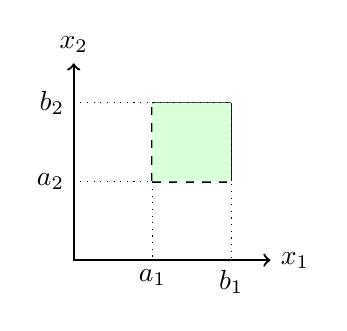
\begin{tikzpicture}
    % Draw axes
    \draw [<->,thick] (0,2.5) node (yaxis) [above] {$x_2$}
        |- (2.5,0) node (xaxis) [right] {$x_1$};

    % Draw two intersecting lines
    \draw[thick, dashed] (1,1) coordinate (a) -- (2,1) coordinate (b);
    \draw[thick, dashed] (a) -- (1,2) coordinate (d);
    \draw[thick]         (d) -- (2,2) coordinate (c);
    \draw[thick]         (b) -- (2,2);

    \fill[green!15] (a) -- (b) -- (c) -- (d) -- (a);

    % Draw lines indicating intersection with y and x axis. Here we 
    % use the perpendicular coordinate system
    \draw[dotted] (yaxis |- a) node[left] {$a_2$}
        -| (xaxis -| a) node[below] {$a_1$};

    \draw[dotted] (yaxis |- c) node[left] {$b_2$}
        -| (xaxis -| c) node[below] {$b_1$};
\end{tikzpicture}

\begin{satz}[Erzeuger der Borelschen $\sigma$-Algebra auf $\mdr^d$]
\label{Satz 1.4}
Es seien $\ce_1,\ce_2,\ce_3$ wie folgt definiert:
\begin{align*}
\ce_1&:=\{(a,b):a,b\in\mdq^d,a\le b\}\\
\ce_2&:=\{(a,b]:a,b\in\mdq^d, a\le b\}\\
\ce_3&:=\{H^-_k(\alpha):\alpha\in\mdq, k=1,\dots,d\}
\end{align*}
Dann gilt:
\[\fb_d=\sigma(\ce_1)=\sigma(\ce_2)=\sigma(\ce_3)\]
Entsprechendes gilt für die anderen Typen von Intervallen und Halbräumen.
\end{satz}

\begin{beweis}
\begin{enumerate}
    \item Sei $G\in\co(\mdr^d), \fm:=\{(a,b):a,b\in\mdq^d,a\le b, (a,b)\subseteq G\}$. 
          Dann ist $\fm$ abzählbar und $G=\bigcup_{I\in\fm}I$. Also 
          gilt:
          \[G\in\sigma(\ce_1)\implies \fb_d=\sigma(\co(\mdr^d))\subseteq\sigma(\ce_1)\]
    \item Sei $(a,b)\in\ce_1$.\\
          \textbf{Fall 1:} $(a,b)=\emptyset\in\ce_2\subseteq\sigma(\ce_2)$\\
          \textbf{Fall 2:} $(a,b)\ne\emptyset, a=(a_1\dots,a_d), b=(b_1\dots,b_d)$.\\
          Dann gilt für alle $j\in\{1,\dots,d\}:a_j<b_j$. Also gilt auch:
\[\exists N\in\mdn:\forall n\ge N: \forall j\in\{1,\dots,d\}:a_j<b_j-\frac1n\]
Definiere $c_n:=(\frac1n,\dots,\frac1n)\in\mdq^d$. Dann gilt:
\[(a,b)=\bigcup_{n\ge N}(a,b-c_n]\in\sigma(\ce_2)\]
Also auch $\ce_1\subseteq\sigma(\ce_2)$ und damit $\sigma(\ce_1)\subseteq\sigma(\ce_2)$.
\item Seien $a = (a_1,\dots,a_d), b=(b_1,\dots,b_d) \in \mdq^d$ mit $a \leq b$. Nachrechnen:
\[(a,b] = \bigcap_{k=1}^d (H^-_k(b_k) \cap H^-_k(a_k)^c) \in \sigma(\ce_3). \]
Das heißt $\ce_2 \subseteq \sigma(\ce_3)$ und damit auch $\sigma(\ce_2) \subseteq \sigma(\ce_3)$. 
\item $H^-_k(\alpha)$ ist abgeschlossen, somit ist $H^-_k(\alpha)^c$ offen und damit $H^-_k(\alpha)^c \in \fb_d$, also auch $H^-_k(\alpha) \in \fb_d$. Damit ist $\ce_3 \subseteq \fb_d \implies \sigma(\ce_3) \subseteq \fb_d$. 
\end{enumerate}
\end{beweis}

\begin{definition}
\index{Spur}
Sei $\emptyset \neq \fm \subseteq \mathcal{P}(X)$ und $\emptyset \neq Y \subseteq X$. 
\[\fm_Y := \{A \cap Y : A \in \fm\}\] 
heißt die \textbf{Spur von $\fm$ in $Y$}.
\end{definition}

\begin{satz}[Spuren und $\sigma$-Algebren]
\label{Satz 1.5}
Sei $\emptyset \neq Y \subseteq X$ und $\fa$ eine $\sigma$-Algebra auf $X$.
\begin{enumerate}
\item $\fa_Y$ ist eine $\sigma$-Algebra auf $Y$.
\item $\fa_Y \subseteq \fa \iff Y \in \fa$
\item Ist $\emptyset \neq \ce \subseteq \mathcal{P}(X)$, so ist $\sigma(\ce_Y) = \sigma(\ce)_Y$.
\end{enumerate}
\end{satz}

\begin{beweis}
\begin{enumerate}
\item \begin{enumerate}
\item[($\sigma_1$)] Es ist $Y=Y\cap X\in\fa_Y$, da $X\in\fa$.
\item[($\sigma_2$)] Sei $B\in\fa_Y$, dann existiert ein $A\in\fa$ mit $B=A\cap Y$. Also ist $Y\setminus B=(X\setminus A)\cap Y\in\fa_Y$, da $X\setminus A\in\fa$ ist.
\item[($\sigma_3$)] Sei $(B_j)$ eine Folge in $\fa_Y$, dann existiert eine Folge $(A_j)\in\fa^\mdn$ mit $B_j=A_j\cap Y$. Es gilt:
\[\bigcup B_j=\bigcup(A_j\cap Y)=(\bigcup A_j)\cap Y\in\fa_Y\]
\end{enumerate}
\item Der Beweis erfolgt durch Implikation in beiden Richtungen:
\begin{enumerate}
\item["`$\implies$"'] Es gilt $Y\in\fa_Y\subseteq\fa$.
\item["`$\impliedby$"'] Sei $B\in\fa_Y$, dann existiert ein $A\in\fa$ mit $B=A\cap Y\in\fa$.
\end{enumerate}
\item Es gilt:
\begin{align*}
\ce\subseteq\sigma(\ce)&\implies\ce_Y\subseteq\sigma(\ce)_Y\\
&\implies\sigma(\ce_Y)\subseteq\sigma(\ce)_Y
\end{align*}
Sei nun:
\[\cd:=\{A\subseteq X:A\cap Y\in\sigma(\ce_Y)\}\]
Übung: $\cd$ ist eine $\sigma$-Algebra auf $X$.\\
Sei $E\in\ce$ dann ist $E\cap Y\in\ce_Y\subseteq\sigma(\ce_Y)$ also $E\in\cd$ und damit $\ce\subseteq\cd$. Daraus folgt:
\begin{align*}
\sigma(\ce)_Y&\subseteq\sigma(\cd)_Y=\cd_Y=\{A\cap Y:A\in\cd\}\\
&\subseteq\sigma(\ce_Y)
\end{align*}
\end{enumerate}
\end{beweis}

\begin{folgerungen}
Sei $X\subseteq\mdr^d$. Dann gilt:
\begin{enumerate}
\item $\fb(X)=(\fb_d)_X$
\item Ist $X\in\fb_d$, so ist $\fb(X)=\{A\in\fb_d:A\subseteq X\}\subseteq\fb_d$.
\end{enumerate}
\end{folgerungen}

\begin{definition}
Wir fügen $\mdr$ das Symbol $+\infty$ hinzu. Es soll gelten:
\begin{enumerate}
\item $\forall a\in\mdr:a<+\infty$
\item $\pm a+(+\infty):=+\infty=:(+\infty)\pm a$
\item $(+\infty)+(+\infty):=+\infty$
\end{enumerate}
Sei etwa $[0,+\infty]:=[0,\infty)\cup\{+\infty\}$.
\begin{enumerate}
\item Sei $(x_n)$ eine Folge in $[0,+\infty]$. Es gilt:
\[x_n\stackrel{n\to\infty}{\to}\infty:\iff \forall c>0\exists n_c\in\mdn:\forall n\ge n_c: x_n> c\]
\item Sei $(a_n)$ eine Folge in $[0,+\infty]$. Es gilt
\[\sum_{n=1}^\infty a_n=\sum a_n = +\infty\]
genau dann wenn $a_j=+\infty$ für ein $j\in\mdn$ oder, falls alle $a_j<+\infty$, wenn $\sum a_n$ divergiert.
\end{enumerate} 
Wegen 13.1 Ana I können Reihen der obigen Form beliebig umgeordnet werden, ohne dass sich ihr Wert verändert.
\end{definition}

\begin{definition}
\index{Maß}
\index{$\sigma$-!Additivität}
\index{Maßraum}
\index{Maß!endliches}
\index{Wahrscheinlichkeitsmaß}\index{Maß!Wahrscheinlichkeits-}
Sei $\fa$ eine $\sigma$-Algebra auf $X$ und $\mu:\fa\to[0,+\infty]$ eine Abbildung. $\mu$ heißt ein \textbf{Maß} auf $\fa$, genau dann wenn gilt:
\begin{enumerate}
\item[$(M_1)$] $\mu(\emptyset)=0$
\item[$(M_2)$] Ist $(A_j)$ eine disjunkte Folge in $\fa$, so ist $\mu(\bigcup A_j)=\sum\mu(A_j)$. Diese Eigenschaft heißt \textbf{$\sigma$-Additivität}.
\end{enumerate}
Ist $\mu$ ein Maß auf $\fa$, so heißt $(X,\fa,\mu)$ ein \textbf{Maßraum}.\\
Ein Maß $\mu$ heißt \textbf{endlich}, genau dann wenn $\mu(X)<\infty$. Ein Maß $\mu$ heißt ein \textbf{Wahrscheinlichkeitsmaß}, genau dann wenn $\mu(X)=1$ ist.
\end{definition}

\begin{beispiel}
\index{Punktmaß}\index{Maß!Punkt-}
\index{Dirac-Maß}\index{Maß!Dirac-}
\index{Zählmaß}\index{Maß!Zähl-}
\begin{enumerate}
\item Sei $\fa=\cp(X)$ und $x_0\in X$. $\delta_{x_0}:\fa\to[0,+\infty]$ sei definiert durch:
\[\delta_{x_0}(A):=
\begin{cases}
1,\ x_0\in A\\
0,\ x_0\not\in A
\end{cases}\]
Klar ist, dass $\delta_{x_0}(\emptyset)=0$ ist.\\
Sei $(A_j)$ eine disjunkte Folge in $\fa$.
\[\delta_{x_0}(\bigcup A_j)=
\left.\begin{cases}
1,\ x_0\in\bigcup A_j\\
0,\ x_0\not\in\bigcup A_j
\end{cases}\right\}=\sum\delta_{x_0}(A_j)\]
$\delta_{x_0}$ ist ein Maß auf $\cp(X)$ und heißt \textbf{Punktmaß} oder \textbf{Dirac-Maß}.
\item Sei $X:=\mdn$, $\fa:=\cp(X)$ und $(p_j)$ eine Folge in $[0,+\infty]$. Definiere $\mu:\fa\to[0,+\infty]$ durch:
\begin{align*}
\mu(A):=
\begin{cases}
0&,A=\emptyset\\
\sum_{j\in A}p_j&,A\ne\emptyset
\end{cases}
\end{align*}
Übung: $\mu$ ist ein Maß auf $\fa=\cp(\mdn)$ und heißt ein \textbf{Zählmaß}. Sind alle $p_j=1$, so ist $\mu(A)$ gerade die Anzahl der Elemente von $A$.
\item Sei $(X,\fa,\mu)$ ein Maßraum, $\emptyset\ne Y\subseteq X$ und $\fa_0\subseteq\fa$ eine $\sigma$-Algebra auf $Y$. Definiere $\mu_0:\fa_0\to[0,+\infty]$ durch $\mu_0(A):=\mu(A)$ ($A\in\fa_0$). Dann ist $(Y,\fa_0,\mu_0)$ ein Maßraum.\\
Ist spezieller $Y\in\fa$, so ist $\fa_0:=\fa_Y\subseteq\fa$ und man definiert $\mu_{|Y}:\fa_Y\to[0,+\infty]$ durch $\mu_{|Y}(A):=\mu(A)$.
\end{enumerate}
\end{beispiel}

\begin{satz}
\label{Satz 1.7}
\((X,\fa,\mu)\) sei ein Maßraum, es seien \(A,B\in\fa\) und \((A_{j})\) sei eine Folge in \(\fa\). Dann:
\begin{enumerate}
\item \(A\subseteq B\,\implies\,\mu(A)\leq\mu(B)\)
\item Ist \(\mu(A)<\infty\) und \(A\subseteq B,\implies\,\mu(B\setminus A)=\mu(B)-\mu(A)\)
\item Ist \(\mu\) endlich, dann ist \(\mu(A)<\infty\) und \(\mu(A^{c})=\mu(X)-\mu(A)\)
\item \(\mu\left(\bigcup A_{j}\right)\leq\sum{\mu(A_{j})}\) (\(\sigma\)-Subadditivität)
\item Ist \(A_{1}\subseteq A_{2}\subseteq A_{3}\subseteq\cdots\), so ist \(\mu(\bigcup A_{j})=\lim_{n\to\infty}{\mu(A_{n})}\)
\item Ist \(A_{1}\supseteq A_{2}\supseteq A_{3}\supseteq\cdots\) und \(\mu(A)<\infty\), so ist
	\(\mu(\bigcap A_{j})=\lim_{n\to\infty}{\mu(A_{n})}\)
\end{enumerate}
\end{satz}
\begin{beweis}
\begin{enumerate}
% Eigentlich muesste es in folgender Zeile statt B=(B\setminus A)\cup A korrekt 
% heissen: B=(B\setminus A)\cupdot A -- Spaeter...
\item[(1)-(3)] \(B=(B\setminus A)\cup A\). Dann: \(\mu(B)=\underbrace{\mu(B\setminus A)}_{\geq0}+\mu(A)\geq\mu(A)\)
\item[(4)] % Das muesste jetzt eigentlich Punkt 4 sein...
\(B_{1}=A_{1},\,B_{k}:=A_{k}\setminus\bigcup_{j=1}^{k-1}{A_{j}}\quad(k\geq 2)\)

Dann: \(B_{j}\in\fa,\,B_{j}\subseteq A_{j}\,(j\in\MdN);\,(B_{j})\) disjunkt und \(\bigcup A_{j}=\bigcup B_{j}\). Dann:
\[
\mu\left(\bigcup A_{j}\right)=\mu\left(\bigcup B_{j}\right)=\sum{\underbrace{\mu(B_{j})}_{\leq\mu(A_{j})}}\leq\sum{\mu(A_{j})}
\]
\item[(5)] % Das muesste jetzt eigentlich Punkt 5 sein...
\(B_{1}=A_{1},\,B_{k}=A_{k}\setminus A_{k-1}\,(k\geq 2)\)

Dann: \(B_{j}\subseteq\fa;\,B_{j}\subseteq A_{j}\,(j\in\MdN);\,\bigcup A_{j}=\bigcup B_{j}\) und \(A_{n}=\bigcup_{j=1}^{n}{B_{j}}\)%\bigcupdot_{j=1}^{n}{B_{j}}\)

Dann: \(\mu(\bigcup A_{j})=\mu(\bigcup B_{j})=\sum{\mu(B_{j})}=\lim_{n\to\infty}{\underbrace{\sum_{j=1}^{n}{\mu(B_{j})}}_{=\mu\left(\bigcup_{j=1}^{n}{B_{j}}\right)=\mu(A_{n})}}\)
\item[(6)] Übung
\end{enumerate}
\end{beweis}

\chapter{Das Lebesgue-Maß}
\label{Kapitel 2}
\index{Lebesgue-Maß}

In diesem Kapitel sei \(X\) eine Menge, \(X\neq\emptyset\).
\begin{definition}
    \index{Ring}
    Sei \(\emptyset\neq \fr \subseteq \cp(X)\). 
    $\fr$ heißt ein \textbf{Ring} (auf \(X\)), genau dann wenn gilt:
    \begin{enumerate}
        \item \(\emptyset \in \fr\)
        \item \(A,B \in \fr \, \implies \; A\cup B, \, B \setminus A \in \fr\)
    \end{enumerate}
\end{definition}

\begin{definition}
    \index{Elementarvolumen}
    \index{Figuren}
    Sei \(d\in\MdN\).
    \begin{enumerate}
        \item \(\ci_{d}:=\Set{(a,b] | a,b \in \MdR^{d}, \, a \leq b}\).
              Seien \(a=(a_{1},\dots,a_{d}),\,b=(b_{1},\dots,b_{d})\in\MdR^d\) 
              und \(I:=(a,b] \in \ci_{d}\)
              \[
              \lambda_{d}(I)= \begin{cases}
                0                                             & \text{falls }I=\emptyset\\
                (b_{1}-a_{1})(b_{2}-a_{2})\cdots(b_{d}-a_{d}) & \text{falls }I\neq\emptyset\end{cases}\quad\text{(\textbf{Elementarvolumen})}
              \]
        \item \(\cf_d:=\left\{\bigcup_{j=1}^{n}I_{j}\mid n\in\MdN,\,I_{1},\dots,I_{n}\in I_{d}\right\}\) (\textbf{Menge der Figuren})
    \end{enumerate}
\end{definition}
Ziel dieses Kapitels: Fortsetzung von \(\lambda_{d}\) auf \(\cf_{d}\) 
und dann auf \(\fb_d\) (\(\leadsto\) Lebesgue-Maß)

Beachte: \(\ci_{d}\subseteq\cf_{d}\subseteq\fb_{d}\overset{1.4}{\implies}\fb_{d}=\sigma(\ci_{d})=\sigma(\cf_{d})\)
\begin{lemma}
    \label{Lemma 2.1}
    Seien \(I,I'\in\ci_{d}\) und \(A\in\cf_{d}\). Dann:
    \begin{enumerate}
        \item \(I\cap I'\in\ci_{d}\)
        \item \(I\setminus I'\in\cf_{d}.\) 
              Genauer: \(\exists\left\{I_{1}',\dots,I_{l}'\right\}\subseteq\ci_{d}\) disjunkt:
              \(I\setminus I'=\bigcup_{j=1}^{l}{I_{j}'}\) % \bigcupdot
        \item \(\exists\left\{I_{1}',\dots,I_{l}'\right\}\subseteq\ci_{d}\) disjunkt: \(A=\bigcup_{j=1}^{l}{I_{j}'}\)
        \item \(\cf_d\) ist ein Ring.
    \end{enumerate}
\end{lemma}

\begin{beweis}
\begin{enumerate}
    \item Sei \(I=\prod_{k=1}^{d}{(a_{k},b_{k}]},\,I'=\prod_{k=1}^{d}{(\alpha_{k},\beta_{k}]};\,\alpha_{k}':=\max\{\alpha_{k},a_{k}\},\,\beta_{k}':=\min\{\beta_{k},b_{k}\}\)

          Ist \(\alpha_{k}'\geq\beta_{k}'\) für ein \(k\in\{1,\dots,d\}\), 
          so ist \(I\cap I'=\emptyset\in\ci_{d}\).
          Sei \(\alpha_{k}'<\beta_{k}'\forall k\in\{1,\dots,d\}\), so
          ist \(I\cap I'=\prod_{k=1}^{d}{(\alpha_{k}',\beta_{k}']\in\ci_{d}}\)
    \item Induktion nach \(d\):
          \begin{itemize}
            \item[I.A.] Klar \checkmark % hier fehlt noch eine Graphik
            \item[I.V.] Die Behauptung gelte für ein \(d\geq 1\)
            \item[I.S.] Seien \(I,I'\in\ci_{d+1}\). Es existieren \(I_{1},I_{1}'\in\ci_{1}\) und \(I_{2},I_{2}'\in\ci_{d}\) mit:
                        \(I=I_{1}\times I_{2},\,I'=I_{1}'\times I_{2}'\)
                        % Graphik einfuegen!

                        Nachrechnen: 
                        \[
                        I\setminus I'=(I_{1}\setminus I_{1}')\times I_{2}\dot \cup(I_{1}\cap I_{1}')\times(I_{2}\setminus I_{2}')
                        \]
                        I.A.\(\implies\,I_{1}\setminus I_{1}'=\) endliche disjunkte Vereinigung von Elementen aus \(\ci_{1}\)\\
                        I.V.\(\implies\,I_{2}\setminus I_{2}'=\) endliche disjunkte Vereinigung von Elementen aus \(\ci_{d}\)\\
                        Daraus folgt die Behauptung für \(d+1\)
          \end{itemize}
    \item Wir zeigen mit Induktion nach \(n\): ist 
          \(A=\bigcup_{j=1}^{n}{I_{j}}\) mit 
          \(I_{1},\dots,I_{d}\in\ci_{d}\), so existiert 
          \(\{I_{1}',\dots,I_{l}'\}\subseteq\ci_{d}\) disjunkt: 
          \(A=\bigcup_{j=1}^{l}{I_{j}'}\)
          \begin{itemize}
            \item[I.A.] \(n=1:\,A=I_{1}\)\checkmark
            \item[I.V.] Die Behauptung gelte für ein \(n\geq 1\)
            \item[I.S.] Sei \(A=\bigcup_{j=1}^{n+1}{I_{j}}\quad(I_{1},\dots,I_{n+1}\in\ci_{d})\)

                        IV\(\,\implies\,\exists\{I_{1}',\dots,I_{l}'\}\subseteq\ci_{d}\) disjunkt:
                        \(\bigcup_{j=1}^{n}{I_{j}}=\bigcup_{j=1}^{l}{I_{j}'}\)	% \bigcupdot...

                        Dann: \(A=I_{n+1}\cup\bigcup_{j=1}^{l}{I_{j}'}=I_{n+1}\cup\bigcup_{j=1}^{l}{(I_{j}'\setminus I_{n+1})}\) % \cupdot...

                        Wende (2) auf jedes \(I_{j}'\setminus I_{n+1}\) an \((j=1,\dots,l)\): 
                        \(I_{j}'\setminus I_{n+1}=\bigcup_{j=1}^{l_{j}}{I_{j}''}\quad(I_{j}''\in\ci_{d})\)

                        Damit folgt:
                        \[
                        A=I_{n+1}\cup\bigcup_{j=1}^{l}{\left(\bigcup_{j=1}^{l_{j}}{I_{j}''}\right)}
                        \]
                        Daraus folgt die Behauptung für \(n+1\).
        \end{itemize}
    \item \((a,a]=\emptyset\implies\emptyset\in\cf_{d}\)

          Seien \(A,B\in\cf_{d}\). Klar: \(A\cup B\in\cf_{d}\)

          Sei \(A=\bigcup_{j=1}^{n}{I_{j}},\,B=\bigcup_{j=1}^{n}{I_{j}'}\quad(I_{j},I_{j}'\in\ci_{d})\). Zu zeigen: \(B\setminus A\in\cf_{d}\)
          \begin{itemize}
            \item[I.A.] \(n=1:\,A=I_{1}\implies B\setminus A=\bigcup_{j=1}^{n}(\underbrace{I_{j}'\setminus I_{j}}_{\in\cf_{d}})\). Wende
                        (2) auf jedes \(I_{j}'\setminus I_{1}\) an. Aus (2) folgt dann \(B\setminus A\in\cf_{d}\).
            \item[I.V.] Die Behauptung gelte für ein \(n\in\MdN\)
            \item[I.S.] Sei \(A'=A\cup I_{n+1}\quad(I_{n+1}\in\ci_{d})\). Dann:
                        \[
                        B\setminus A'=\underbrace{(B\setminus A)}_{\in\cf_{d}}\setminus\underbrace{I_{n+1}}_{\in\cf_{d}}\in\cf_{d}
                        \]
          \end{itemize}
  \end{enumerate}
\end{beweis}

\begin{lemma}
    \label{Lemma 2.2}
    Sei \(A\in\cf_{d}\) und \(\{I_{1},\dots,I_{n}\}\subseteq\ci_{d}\) disjunkt und
    \(\{I_{1}',\dots,I_{m}'\}\subseteq\ci_{d}\) disjunkt mit 
    \(\bigcup_{j=1}^{n}{I_{j}}=A=\bigcup_{j=1}^{m}{I_{j}'}\). Dann:
    \[
    \sum_{j=1}^{n}{\lambda_{d}(I_{j})}=\sum_{j=1}^{m}{\lambda_{d}(I_{j}')}
    \]
\end{lemma}
\begin{definition}
    Sei \(A\in\cf_{d}\) und \(A=\bigcup_{j=1}^{n}{I_{j}}\) mit 
    \(\{I_{1},\dots,I_{n}\}\subseteq\ci_{d}\)
    disjunkt (beachte Lemma \ref{Lemma 2.1}, Punkt 3).
    \[
    \lambda_{d}(A):=\sum_{j=1}^{n}{\lambda_{d}(I_{j})}
    \]
    Wegen Lemma \ref{Lemma 2.2} ist \(\lambda_{d}:\cf_{d}\to[0,\infty)\)
    wohldefiniert.
\end{definition}
\begin{satz}
    \label{Satz 2.3}
    Seien \(A,B\in\cf_{d}\) und \((B_{n})\) sei eine Folge in \(\cf_{d}\).
    \begin{enumerate}
        \item \(A\cap B=\emptyset\implies\lambda_{d}(A\cup B)=\lambda_{d}(A)+\lambda_{d}(B)\)
        \item \(A\subseteq B\implies\lambda_{d}(A)\leq\lambda_{d}(B)\)
        \item \(\lambda_{d}(A\cup B)\leq\lambda_{d}(A)+\lambda_{d}(B)\)
        \item Sei \(\delta>0\). Es existiert \(C\in\cf_{d}:\overline{C}\subseteq B\) 
              und \(\lambda_{d}(B\setminus C)\leq\delta\).
        \item Ist \(B_{n+1}\subseteq B_{n}\forall n\in\mdn\) und 
              \(\bigcap B_{n}=\emptyset\), so gilt: 
              \(\lambda_{d}(B_{n})\to 0\,(n\to \infty)\)
    \end{enumerate}
\end{satz}

\begin{beweis}
\begin{enumerate}
\item Aus Lemma \ref{Lemma 2.1} folgt: Es existiert 
\(\{I_{1},\dots,I_{n}\}\subseteq\ci_{d}\)
disjunkt und es existiert \(\{I_{1}',\dots,I_{m}'\}\subseteq\ci_{d}\) disjunkt:
\(A=\bigcup_{j=1}^{n}{I_{j}},\,B=\bigcup_{j=1}^{m}{I_{j}'}\).

\(J:=\{I_{1},\dots,I_{n},I_{1}',\dots,I_{m}'\}\subseteq\ci_{d}\). Aus 
\(A\cap B=\emptyset\) folgt: \(J\) ist disjunkt. Dann: 
\(A\cup B=\bigcup_{I\in J}{I}\)	% Hier auch wieder: \bigcupdot

Also:
\begin{align*}
\lambda_{d}(A\cup B)&=\sum_{I\in J}{\lambda_{d}(I)}\\
    &=\sum_{j=1}^{n}{\lambda_{d}(I_{j})}+\sum_{j=1}^{m}{\lambda_{d}(I_{j}')}\\
    &=\lambda_{d}(A)+\lambda_{d}(B)
\end{align*}
\item wie bei Satz \ref{Satz 1.7}
\item \(\lambda_{d}(A\cup B)=\lambda(A\cup(B\setminus A))\overset{(1)}{=}\lambda_{d}(A)+\lambda_{d}(B\setminus A)\overset{(2)}{\leq}\lambda_{d}(A)+\lambda_{d}(B)\) % \cupdot...
\item Übung; es genügt zu betrachten: \(B\in\ci_{d}\) % Graphik einfuegen
\item Sei \(\varepsilon>0\). Aus (4) folgt: Zu jedem \(B_{n}\) existiert ein
\(C_{n}\in\cf_{d}:\overline{C}_{n}\subseteq B_{n}\) und
\begin{equation}
\label{eq: Abschaetzung Mass -- Beweis Satz 2.3.(5)}
\lambda_{d}(B_{n}\setminus C_{n})\leq\frac{\varepsilon}{2^{n}}
\end{equation}
Dann:
\(\bigcap{\overline{C}_{n}}\subseteq\bigcap{B_{n}}=\emptyset\implies\bigcup{\overline{C}_{n}^{c}}=\mdr^{d}\implies\underbrace{\overline{B}_{1}}_{\text{kompakt}}\subseteq\bigcup{\underbrace{\overline{C}_{n}^{c}}_{\text{offen}}}\)

Aus der Definition von Kompaktheit (Analysis II, \S 2) folgt:
\(\exists m\in\mdn:\,\bigcup_{j=1}^{m}{\overline{C}_{j}^{c}}\supseteq\overline{B}_{1}\)
Dann: \(\bigcap_{j=1}^{m}{\overline{C}_{j}}\subseteq\overline{B}_{1}^{c}\).
Andererseits: \(\bigcap_{j=1}^{m}{\overline{C}_{j}}\subseteq\bigcap_{j=1}^{m}{B_{j}}\subseteq B_{1}\subseteq\overline{B}_{1}\). 

Also: \(\bigcap_{j=1}^{m}{\overline{C}_{j}}=\emptyset\). Das heißt:
\(\bigcap_{j=1}^{n}{\overline{C}_{j}}=\emptyset\,\forall n\geq m\)

\(D_{n}:=\bigcap_{j=1}^{n}{C_{j}}\). Dann: \(D_{n}=\emptyset\,\forall n\geq m\)

\textbf{Behauptung:} \(\lambda_{d}(B_{n}\setminus D_{n})\leq\left(1-\frac{1}{2^{n}}\right)\ep\,\forall n\in\mdn\)
\begin{beweis}
\begin{itemize}
\item[I.A.] \(\lambda_{d}(B_{1}\setminus D_{1})=\lambda_{d}(B_{1}\setminus C_{1})\overset{\eqref{eq: Abschaetzung Mass -- Beweis Satz 2.3.(5)}}{\leq}\frac{\ep}{2}=\left(1-\frac{1}{2}\right)\ep\) \checkmark
\item[I.V.] Die Behauptung gelte für ein \(n\in\mdn\).
\item[I.S.] \begin{align*}
    \lambda_{d}(B_{n+1}\setminus D_{n+1})&=\lambda_{d}\left((B_{n+1}\setminus D_{n})\cup(B_{n+1}\setminus C_{n+1})\right)\\
    &\overset{(3)}{\leq}\lambda_{d}(\underbrace{B_{n+1}\setminus D_n}_{\subseteq B_{n}\setminus D_{n}})+\underbrace{\lambda_{d}(B_{n+1}\setminus C_{n+1})}_{\overset{\eqref{eq: Abschaetzung Mass -- Beweis Satz 2.3.(5)}}{\leq}\frac{\ep}{2^{n+1}}}\\
    &\overset{(2)}{\leq}\lambda_{d}(B_{n}\setminus D_{n})+\frac{\ep}{2^{n+1}}\\
    &\overset{\text{I.V.}}{\leq}\left(1-\frac{1}{2^{n}}\right)+\frac{\ep}{2^{n+1}}\\
&=\left(1-\frac{1}{2^{n+1}}\right)\ep
    \end{align*}
\end{itemize}
\end{beweis}

Für \(n\geq m:\,D_{n}=\emptyset\,\implies\,\lambda_{d}(B_{n})=\lambda_{d}(B_{n}\setminus D_{n})\leq\left(1-\frac{1}{2^{n}}\right)\varepsilon\leq\varepsilon\)
\end{enumerate}
\end{beweis}

\begin{definition}
\index{Prämaß}
Es sei \(\fr\) ein Ring auf \(X\). Eine Abbildung \(\mu:\fr\to[0,\infty]\) 
heißt ein \textbf{Prämaß} \ auf \(\fr\), wenn gilt:
\begin{enumerate}
\item \(\mu(\emptyset)=0\)
\item Ist \(A_{j}\) eine disjunkte Folge in \(\fr\) und \(\bigcup{A_{j}}\in\fr\), so ist \(\mu\left(\bigcup{A_{j}}\right)=\sum{\mu(A_{j})}\).
\end{enumerate}
\end{definition}

\begin{satz}
\label{Satz 2.4}
\(\lambda_{d}:\cf_{d}\to[0,\infty]\) ist ein Prämaß.
\end{satz}
\begin{beweis}
\begin{enumerate}
\item Klar: \(\lambda_{d}(\emptyset)=0\)
\item Sei \(A_{j}\) eine disjunkte Folge in \(\cf_{d}\) und \(A:=\bigcup{A_{j}}\in\cf_{d}\).

\(B_{n}:=\bigcup_{j=n}^{\infty}{A_{j}}\,(n\in\mdn)\); \((B_{n})\) hat die
Eigenschaften aus \ref{Satz 2.3}, Punkt 5. Also: \(\lambda_{d}(B_{n})\to 0\).

Für \(n\geq 2\):
\[
\lambda_{d}(A)=\lambda_{d}(A_{1}\cup\cdots\cup A_{n-1}\cup B_{n})\overset{\ref{Satz 2.3}.(1)}{=}\sum_{j=1}^{n-1}{\lambda_{d}(A_{j})}+\lambda_{d}(B_{n})
\]
Daraus folgt: 
\[
\sum_{j=1}^{n-1}{\lambda_{d}(A_{j})}=\lambda_{d}(A)-\lambda_{d}(B_{n})\quad\forall n\geq 2
\]
Mit \(n\to\infty\) folgt die Behauptung.
\end{enumerate}
\end{beweis}

\begin{satz}[Fortsetzungssatz von Carath\'eodory]
\label{Satz 2.5}
Sei \(\fr\) ein Ring auf \(X\) und \(\mu:\fr\to[0,\infty]\) ein Prämaß. Dann
existiert ein Maßraum \((X,\fa(\mu),\overline{\mu})\) mit
\begin{enumerate}
\item \(\sigma(\fr)\subseteq\fa(\mu)\)
\item \(\overline{\mu}(A)=\mu(A)\,\forall A\in\fr\)
\end{enumerate}
Insbesondere: \(\overline{\mu}\) ist ein Maß\ auf \(\sigma(\fr)\).
\end{satz}

\begin{satz}[Eindeutigkeitssatz]
\label{Satz 2.6}
Sei \(\emptyset\neq\ce\subseteq\cp(X)\), es seien \(\nu,\,\mu\) Maße auf
\(\sigma(\ce)\) und es gelte: \(\mu(E)=\nu(E)\,\forall E\in\ce\).

Weiter gelten:
\begin{enumerate}
\item \(E,F\in\ce\implies E\cap F\in\ce\quad\text{(durchschnittstabil)}\)
\item Es existiert eine Folge \((E_{n})\) in \(\ce\): \(\bigcup{E_{n}}=X\) und
\(\mu(E_{n})<\infty\forall n\in\mdn\).
\end{enumerate}
Dann: \(\mu=\nu\) auf \(\sigma(\ce)\).
\end{satz}

\begin{satz}%[Lebesgue-Maß]
\label{Satz 2.7}
\index{Lebesgue-Maß}
Es gibt genau eine Fortsetzung von \(\lambda_{d}:\cf_{d}\to[0,\infty]\) auf
\(\fb_{d}\) zu einem Maß. Diese Fortsetzung heißt \textbf{Lebesgue-Maß} \ (L-Maß)
und wird ebenfalls mit \(\lambda_{d}\) bezeichnet.
\end{satz}
\begin{beweis}
Aus Lemma \ref{Lemma 2.1} und Satz \ref{Satz 2.4} folgt: \(\lambda_{d}\) ist ein
Prämaß\ auf \(\fr:=\cf_{d}\); es ist \(\sigma(\fr)=\fb_{d}\).

Aus Satz \ref{Satz 2.5} folgt: \(\lambda_{d}\) kann zu einem Maß\ auf 
\(\fb_{d}\) fortgesetzt werden.

Sei \(\nu\) ein weiteres Maß\ auf \(\fb_{d}\) mit: 
\(\nu(A)=\lambda_{d}(A)\,\forall A\in\cf_{d}\). \(\ce:=\ci_{d}\). Dann:
\(\sigma(\ce)\overset{\ref{Satz 1.4}}{=}\fb_{d}\).
\begin{enumerate}
\item \(E,F\in\ce\overset{\ref{Lemma 2.1}}{\implies}E\cap F\in\ce\)
\item \(E_{n}:=(-n,n]^{d}\)

Klar: 
\begin{align*}
\bigcup E_{n}&=\mdr^{d}\\
\lambda_{d}(E_{n})&=(2n)^{d}<\infty
\end{align*}
\end{enumerate}
Klar: \(\nu(E)=\lambda_{d}(E)\,\forall E\in\ce\). Mit Satz \ref{Satz 2.6} folgt
dann: \(\nu=\lambda_{d}\) auf \(\fb_{d}\).
\end{beweis}

\begin{bemerkung}
Sei \(X\in\fb_{d}\). Aus 1.6 folgt: \(\fb(X)=\{A\in\fb_{d}\mid A\subseteq X\}\).
Die Einschränkung von \(\lambda_{d}\) auf \(\fb(X)\) heißt ebenfalls
L-Maß\ und wird mit \(\lambda_{d}\) bezeichnet.
\end{bemerkung}

\begin{beispieleX}
\begin{enumerate}
\item Seien \(a=(a_{1},\dots,a_{d}),\,b=(b_{1},\dots,b_{d})\in\mdr^{d},\,a\leq b\) und \(I=[a,b]\).\\
\textbf{Behauptung}\\\(\lambda_{d}([a,b])=(b_{1}-a_{1})\cdots(b_{d}-a_{d})\) (Entsprechendes gilt für \((a,b)\) und \([a,b)\))
\begin{beweis}
\(I_{n}:=(a_{1}-\frac{1}{n},b_{1}]\times\cdots\times(a_{d}-\frac{1}{n},b_{d}];\,I_{1}\supset I_{2}\supset\cdots;\,\bigcap I_{n}=I,\,\lambda_{d}(I_{1})<\infty\)

Aus Satz \ref{Satz 1.7}, Punkt 5, folgt:
\begin{align*}
\lambda_{d}(I)&=\lim_{n\to\infty}{\lambda_{d}(I_{n})}\\
&=\lim_{n\to\infty}{(b_{1}-a_{1}+\frac{1}{n})\cdots(b_{d}-a_{d}+\frac{1}{n})}\\
&=(b_{1}-a_{1})\cdots(b_{d}-a_{d})
\end{align*}
\end{beweis}
\item Sei \(a\in\mdr^{d},\,\{a\}=[a,a]\in\fb_{d}\). Aus obigem Beispiel (1)
folgt: \(\lambda_{d}(\{a\})=0\).
\item \(\mdq^{d}\) ist abzählbar, also: \(\mdq^{d}=\{a_{1},a_{2},\dots\}\)
mit \(a_{j}\neq a_{i}\,(i\neq j)\). Dann: \(\mdq^{d}=\bigcup\{a_{j}\}\) %\bigcupdot...

Dann gilt: \(\mdq^{d}\in\fb_{d}\) und \(\lambda_{d}(\mdq^{d})=\sum{\lambda_{d}(\{a_{j}\})}=0\).
\item Wie in Beispiel (3): Ist \(A\subseteq\mdr^{d}\) abzählbar, so ist
\(A\in\fb_{d}\) und \(\lambda_{d}(A)=0\).
\item Sei \(j\in\{1,\dots,d\}\) und \(H_{j}:=\{(x_{1},\dots,x_{d})\in\mdr^{d}\mid x_{j}=0\}\). \(H_{j}\) ist abgeschlossen, damit folgt: \(H_{j}\in\fb_{d}\).

Ohne Beschränkung der Allgemeinheit sei \(j=d\). Dann:
\(I_{n}:=\underbrace{[-n,n]\times\cdots\times[-n,n]}_{(d-1)-\text{mal}}\times\{0\}\).
% Hier fehlt noch eine Graphik
Aus Beispiel (1) folgt: \(\lambda_{d}(I_{n})=0\).

Aus \(H_{d}=\bigcup{I_{n}}\) folgt: \(\lambda_{d}(H_{d})\leq\sum{\lambda_{d}(I_{n})}=0\). Also: \(\lambda_{d}(H_{j})=0\).
\end{enumerate}
\end{beispieleX}

\begin{definition}
Sei $x\in\mdr^d, B\subseteq\mdr^d$. Definiere:
\[x+B:=\{x+b\mid b\in B\}\]
\end{definition}

\begin{beispiel}
Ist $I\in\ci_d$, so gilt $x+I\in\ci_d$ und $\lambda_d(x+I)=\lambda_d(I)$.
\end{beispiel}

\begin{satz}
\label{Satz 2.8}
Sei $x\in\mdr^d, \fa:=\{B\in\fb_d:x+B\in\fb_d\}$ und $\mu:\fa\to[0,\infty]$ sei definiert durch $\mu(A):=\lambda_d(x+A)$. Dann gilt:
\begin{enumerate}
\item $(\mdr^d,\fa,\mu)$ ist ein Maßraum.
\item Es ist $\fa=\fb_d$ und $\mu=\lambda_d$ auf $\fb_d$. D.h. für alle $A\in\fb_d$ ist $x+A\in\fb_d$ und $\lambda_d(x+A)=\lambda_d(A)$ (Translationsinvarianz des Lebesgue-Maßes).
\end{enumerate}
\end{satz}

\begin{beweis}
\begin{enumerate}
\item Leichte Übung!
\item Es ist klar, dass $\fb_d\supseteq\fa$. Nach dem Beispiel von oben gilt:
\[\ci_d\subseteq\fa\subseteq\fb_d=\sigma(\ci_d)\subseteq\sigma(\fa)=\fa\]
Setze $\ce:=\ci_d$, dann ist $\sigma(\ce)=\fb_d$ und es gilt nach dem Beispiel von oben:
\[\forall E\in\ce:\mu(E)=\lambda_d(E)\]
$\ce$ hat die Eigenschaften (1) und (2) aus Satz \ref{Satz 2.6}, daraus folgt dann, dass $\mu=\lambda_d$ auf $\fb_d$ ist.
\end{enumerate}
\end{beweis}

\begin{satz}
\label{Satz 2.9}
Sei $\mu$ ein Maß auf $\fb_d$ mit der Eigenschaft:
\[\forall x\in\mdr^d, A\in\fb_d:\mu(A)=\mu(x+A)\]
Weiter sei $c:=\mu((0,1]^d)<\infty$. Dann gilt:
\[\mu=c\cdot\lambda_d\]
\end{satz}

\begin{satz}[Regularität des Lebesgue-Maßes]
\label{Satz 2.10}
Sei $A \in\fb_d$, dann gilt:
\begin{enumerate}
\item
$\lambda_d(A)=\inf\left\{\lambda_d(G)\mid G\subseteq\mdr^d\text{ offen und }A \subseteq G\right\}\\
 =\inf\left\{\lambda_d(V)\mid V=\bigcup_{j=1}^\infty I_j, I_j\subseteq\mdr^d\text{ offenes Intervall }, A\subseteq V\right\}$
\item $\lambda_d(A)=\sup\{\lambda_d(K)\mid K\subseteq\mdr^d\text{ kompakt }, K\subseteq A\}$
\end{enumerate}
\end{satz}

\begin{beweis}
\begin{enumerate}
\item Ohne Beweis.
\item Setze $\beta:=\sup\{\lambda_d(K)\mid K\subseteq\mdr^d\text{ kompakt }, K\subseteq A\}$. Sei $K$ kompakt und $K\subseteq A$, dann gilt $\lambda_d(K)\le\lambda_d(A)$, also ist auch $\beta\le\lambda_d(A)$.

\textbf{Fall 1:} Sei $A$ zusätzlich beschränkt.\\
Sei $\ep>0$. Es existiert ein $r>0$, sodass $A\subseteq B:=\overline{U_r(0)}\subseteq[-r,r]^d$ ist, dann gilt:
\[\lambda_d(A)\le\lambda_d([-r,r]^d)=(2r)^d<\infty\]
Aus (1) folgt, dass eine offene Menge $G\supseteq B\setminus A$ existiert mit $\lambda_d(G)\le\lambda_d(B\setminus A)+\ep$. Dann gilt nach \ref{Satz 1.7}:
\[\lambda_d(B\setminus A)=\lambda_d(B)-\lambda_d(A)\]
Setze nun $K:=B\setminus G=B\cap G^c$, dann ist $K$ kompakt und $K\subseteq B\setminus(B\setminus A)=A$. Da $B\subseteq G\cup K$ ist, gilt:
\[\lambda_d(B)\le\lambda_d(G\cup K)\le \lambda_d(B)-\lambda_d(A)+\ep+\lambda_d(K)\]
Woraus folgt:
\[\lambda_d(A)\le\lambda_d(K)+\ep\]

\textbf{Fall 2:} Sei $A\in\fb_d$ beliebig.\\
Setze $A_n:=A\cap\overline{U_n(0)}$. Dann ist $A_n$ für alle $n\in\mdn$ beschränkt, $A_n\subseteq A_{n+1}$ und $A=\bigcup_{n\in\mdn} A_n$. Nach \ref{Satz 1.7} gilt:
\[\lambda_d(A)=\lim\lambda_d(A_n)\]
Aus Fall 1 folgt, dass für alle $n\in\mdn$ ein kompaktes $K_n\subseteq A_n$ mit $\lambda_d(A_n)\le\lambda_d(K_n)+\frac1n$ existiert. Dann gilt:
\[\lambda_d(A_n)\le\lambda_d(K_n)+\frac1n\le\lambda_d(A)+\frac1n\]
Also auch:
\[\lambda_d(A)=\lim\lambda(K_n)\le\beta\]
\end{enumerate}
\end{beweis}

\textbf{Auswahlaxiom:}\\
Sei $\emptyset\ne\Omega$ Indexmenge, es sei $\{X_\omega\mid \omega\in\Omega\}$ ein disjunktes System von nichtleeren Mengen $X_\omega$. Dann existiert ein $C\subseteq\bigcup_{\omega\in\Omega}X_\omega$, sodass $C$ mit jedem $X_j$ genau ein Element gemeinsam hat.

\begin{satz}[Satz von Vitali]
\label{Satz 2.11}
Es existiert ein $C\subseteq\mdr^d$ sodass $C\not\in\fb_d$.
\end{satz}

\begin{beweis}
Wir definieren auf $[0,1]^d$ eine Äquivalenzrelation $\sim$, durch:
\begin{align*}
\forall x,y\in[0,1]^d: x \sim y\iff x-y\in\mdq^d\\
\forall x\in[0,1]^d:[x]:=\{y\in[0,1]^d\mid x\sim y\}
\end{align*}
Nach dem Auswahlaxiom existiert ein $C\subseteq[0,1]^d$, sodass $C$ mit jedem $[x]$ genau ein Element gemeinsam hat.
Es ist $\mdq^d\cap[-1,1]^d=\{q_1,q_2,\dots\}$ mit $q_i\ne q_j$ für $(i\ne j)$. Dann gilt:
\begin{align*}
\tag{1} \bigcup_{n=1}^\infty(q_n+C)\subseteq[-1,2]^d\\
\tag{2} [0,1]^d\subseteq\bigcup_{n=1}^\infty(q_n+C)
\end{align*}
\begin{beweis}
Sei $x\in[0,1]^d$. Wähle $y\in C$ mit $y\in[x]$, dann ist $x\sim y$, also $x-y\in\mdq^d\cap[-1,1]^d$. D.h.:
\[\exists n\in\mdn: x-y=q_n\implies x=q_n+y\in q_n+C\] 
\end{beweis}
Außerdem ist $\{q_n+C\mid n\in\mdn\}$ disjunkt.
\begin{beweis}
Sei $z\in(q_n+C)\cap(q_m+C)$, dann existieren $a,b\in\mdq^d$, sodass gilt:
\begin{align*}
(q_n+a=z=q_m+b) &\implies (b-a=q_m-q_n\in\mdq^d)\\
&\implies (a\sim b) \implies([a]=[b])\\
&\implies (a=b)\implies (q_n=q_m)
\end{align*}
\end{beweis}
\textbf{Annahme:} $C\in\fb_d$, dann gilt nach (1):
\begin{align*}
3^d&=\lambda_d([-2,1]^d)\\
&\ge\lambda_d(\bigcup(q_n+C))\\
&=\sum \lambda_d(q_n+C)\\
&=\sum \lambda_d(C)
\end{align*}
Also ist $\lambda_d(C)=0$. Damit folgt aus (2):
\begin{align*}
1&=\lambda_d([0,1]^d)\\
&\le \lambda_d(\bigcup (q_n+C))\\
&=\sum \lambda_d(C)\\
&=0
\end{align*}
\end{beweis}

\chapter{Messbare Funktionen}
\label{Kapitel 3}

In diesem Paragraphen seien $\emptyset\ne X,Y,Z$ Mengen.

\begin{definition}
\index{messbar!Raum}\index{Raum!messbarer}
Ist $\fa$ eine $\sigma$-Algebra auf $X$, so heißt $(X,\fa)$ ein \textbf{messbarer Raum}.
\end{definition}

\begin{definition}
\index{$\fa$-$\fb$-messbar}
\index{messbar!Funktion}
Sei $\fa$ eine $\sigma$-Algebra auf $X$, $\fb$ eine $\sigma$-Algebra auf $Y$ und $f:X\to Y$ eine Funktion. $f$ heißt genau dann \textbf{$\fa$-$\fb$-messbar}, wenn gilt:
\[\forall B\in\fb: f^{-1}(B)\in\fa\]
\end{definition}

\begin{bemerkung}
Seien die Bezeichnungen wie in obiger Definition, dann gilt:
\begin{enumerate}
\item $f$ sei $\fa$-$\fb$-messbar, $\fa'$ eine weitere $\sigma$-Algebra auf $X$ mit $\fa\subseteq\fa'$ und $\fb'$ sei eine $\sigma$-Algebra auf $Y$ mit $\fb'\subseteq\fb$.\\
Dann ist $f$ $\fa'$-$\fb'$-messbar.
\item Sei $X_0\in\fa$, dann gilt $\fa_{X_0}\subseteq\fa$ nach \ref{Satz 1.5}. Nun sei $f:X\to Y$ $\fa$-$\fb$-messbar, dann ist $f_{\mid X_0}:X_0\to Y$ $\fa_{X_0}$-$\fb$-messbar.
\end{enumerate}
\end{bemerkung}

\begin{beispiel}
\begin{enumerate}
\item Sei $\fa$ eine $\sigma$-Algebra auf $X$ und $A\subseteq X$. $\mathds{1}_A:X\to\mdr$ ist genau dann $\fa$-$\fb_1$-messbar, wenn $A\in\fa$ ist.
\item Sei $X=\mdr^d$. Ist $A\in\fb_d$, so ist $\mathds{1}_A$ $\fb_d$-$\fb_1$-messbar.
\item Ist $C$ wie in \ref{Satz 2.11}, so ist $\mathds{1}_C$ nicht $\fb_d$-$\fb_1$-messbar.
\item Es sei $f:X\to Y$ eine Funktion und $\fb$ ($\fa$) eine $\sigma$-Algebra auf $Y$ ($X$), dann ist $f$ $\cp(X)$-$\fb$-messbar ($\fa$-$\{Y,\emptyset\}$-messbar).
\end{enumerate}
\end{beispiel}

\begin{satz}
\label{Satz 3.1}
Seien \(\fa,\,\fb,\,\fc\) \(\sigma\)-Algebren auf \(X,\,Y\) bzw. \(Z\). Weiter seien \(f:\,X\to Y\) und \(g:\,Y\to Z\)
Funktionen.
\begin{enumerate}
\item Ist \(f\) \(\fa-\fb-\)messbar und ist \(g\) \(\fb-\fc-\)messbar, so ist \(g\circ f:\,X\to Z\) \(\fa-\fc-\)messbar.
\item Sei \(\emptyset\neq\ce\subseteq\cp(Y)\) und \(\sigma(\ce)=\fb\). Dann:
\begin{center}
\(f\) ist \(\fa-\fb-\)messbar, genau dann, wenn gilt: \(\forall E\in\ce:\,f^{-1}(E)\in\fa\)
\end{center}
\end{enumerate}
\end{satz}

\begin{beweis}
\begin{enumerate}
\item Sei \(C\in\fc\); \(g\) ist messbar, daraus folgt \(g^{-1}(C)\in\fb\);
\(f\) ist messbar, daraus folgt \(f^{-1}(g^{-1}(C))=(g\circ f)^{-1}(C)\in\fa\)
\item \begin{itemize}
\item[\(\Rightarrow\)] \checkmark
\item[\(\Leftarrow\)] \(\fd:=\{B\subseteq Y\mid f^{-1}(B)\in\fa\}\)
Übung: \(\fd\) ist eine \(\sigma\)-Algebra auf \(Y\).

Aus der Voraussetzung folgt: \(\ce\subseteq\fd\).
Dann: \(\fb=\sigma(\ce)\subseteq\fd\). Ist \(B\in\fb\), so ist \(B\in\fd\), also
\(f^{-1}(B)\in\fa\).
\end{itemize}
\end{enumerate}
\end{beweis}

\begin{definition}
\index{messbar!Borel}\index{messbar}
Sei \(X\in\fb_{d}\). Ist \(f:\,X\to\mdr^{k}\) \(\fb(X)-\fb_{k}-\)messbar, so heißt \(f\) \textbf{(Borel-)messbar}.
\end{definition}
Ab jetzt sei stets \(X\in\fb_{d}\). (Erinnerung: \(\fb(X)=\{A\in\fb_{d}\mid A\subseteq X\}\))

\begin{satz}
\label{Satz 3.2}
Seien \(f,\,g:\,X\to\mdr^{k}\) und \(\alpha,\beta\in\mdr\).
\begin{enumerate}
\item Ist \(f\) auf \(X\) stetig, so ist \(f\) messbar.
\item Ist \(f=(f_{1},\dots,f_{k})\), so gilt: \(f\) ist messbar \(\Leftrightarrow\) alle \(f_{j}\) sind messbar.
\item Sind \(f\) und \(g\) messbar, so ist \(\alpha f+\beta g\) messbar.
\item Sei \(k=1\) und \(f\) und \(g\) seien messbar. Dann:
\begin{enumerate}
\item \(fg\) ist messbar
\item Ist \(f(x)\neq0\forall x\in X\), so ist \(\frac{1}{f}\) messbar
\item \(\{x\in X\mid f(x)\geq g(x)\}\in\fb(X)\)
\end{enumerate}
\end{enumerate}
\end{satz}

\begin{beweis}
\begin{enumerate}
\item Sei \(G\in\co(\mdr^{k})\). Mit \(f\) stetig folgt: \(f^{-1}(G)\in\co(X)\in\fb(X)\)

\(\sigma(\co(\mdr^{k}))=\fb_{k}\). Die Behauptung folgt aus \ref{Satz 3.1}.(2).
\item \begin{itemize}
\item[\(\Leftarrow:\)] Sei \(I=(a,b]=\prod_{j=1}^{k}{(a_{j},b_{j}]}\in I_{k}\quad (a=(a_{1},\dots,a_{k}),\,b=(b_{1},\dots,b_{k}),\,a\leq b)\)

Dann: \(f^{-1}(I)=\bigcap_{j=1}^{k}{\underbrace{f_{j}^{-1}(\underbrace{(a_{j},b_{j}]}_{\in\fb_{1}}}_{\in\fb(X)}}\in\fb(X)\)

Aus \(\sigma(I_{k})=\fb_{k}\) folgt mit \ref{Satz 3.1}.(2): \(f\) ist messbar.
\item[\(\Rightarrow:\)] Für \(j=1,...,k\) sei \(p_{j}:\mdr^{k}\to\mdr\) definiert durch 
\(p_{j}(x_{1},\dots,x_{k}):=x_{j}\)

\(p_{j}\) ist stetig, also messbar (nach (1)). Es ist \(f_{j}=p_{j}\circ f\). Mit \ref{Satz 3.1}.(1) folgt: \(f_{j}\) ist
messbar.
\end{itemize}
\item \(h:=(f,g):\,X\to\mdr^{2k}\); aus (2): \(h\) ist messbar.

\(\vp(x,y):=\alpha x+\beta y\,(x,y\in\mdr^{k})\)

\(\vp\) ist stetig, also messbar (nach (1)). Es ist \(\alpha f+\beta g=\vp\circ h\). Mit \ref{Satz 3.1}.(1) folgt: 
\(\alpha f+\beta g\) ist messbar.
\item 
\begin{enumerate}
\item \(h:=(f,g):\,X\to\mdr^{2k}\) ist messbar (nach (2)); \(\vp(x,y):=xy\), \(\vp\) ist stetig, also messbar.

Es ist \(fg=\vp\circ h\). Mit \ref{Satz 3.1}.(1) folgt: \(fg\) ist messbar.
\item \(\vp(x):=\frac{1}{x}\), \(\vp\) ist stetig auf \(\mdr\setminus\{0\}\), also messbar.

\(\frac{1}{f}=\vp\circ f\). Mit \ref{Satz 3.1}.(1) folgt: \(\frac{1}{f}\) ist messbar.
\item \(A:=\{x\in X\mid f(x)\geq g(x)\}=\{x\in X\mid f(x)-g(x)\in[0,\infty)\}=\underbrace{(f-g)}_{\text{messbar nach (3)}}^{-1}(\overbrace{[0,\infty)}^{\in\fb_{1}})\in\fb(X)\)
\end{enumerate}
\end{enumerate}
\end{beweis}

\begin{folgerungen}
\label{Folgerung 3.3}
\begin{enumerate}
\item Seien \(A,\,B\in\fb(X),\,A\cap B=\emptyset\) und \(X=A\cup B\). Weiter seien \(f:A\to\mdr^{k}\) und
\(g:B\to\mdr^{k}\) messbar. Dann ist \(h:X\to\mdr^{k}\), definiert durch 
\[
h(x):=\begin{cases}f(x)&x\in A\\g(x)&x\in B\end{cases},
\]
messbar.
\item Ist \(f:X\to\mdr^{k}\) messbar und \(g(x):=\lVert f(x)\rVert\,(x\in X)\), so ist \(g\) messbar.
\end{enumerate}
\end{folgerungen}

\begin{beweis}
\begin{enumerate}
\item Sei \(C\in\fb_{k}\). Dann:
\[
h^{-1}(C)=\underbrace{f^{-1}(C)}_{\in\fb(A)\subseteq\fb(X)}\cup\underbrace{g^{-1}(C)}_{\in\fb(B)\subseteq\fb(X)}\in\fb(X)
\]
\item Definiere \(\vp(z)=\lVert z\rVert\quad(z\in\mdr^{k})\); \(\vp\) ist
stetig, also messbar.

Es ist \(g=\vp\circ f\). Mit \ref{Satz 3.1} folgt: \(g\) ist messbar.
\end{enumerate}
\end{beweis}

\begin{beispiel}
\(X=\mdr^{2},\,f(x,y):=\begin{cases}\frac{\sin(y)}{x}&x\neq 0\\0&x=0\end{cases}\)

für \(x\neq 0:\,f(x,x)=\frac{\sin(X)}{x}\overset{x\to 0}{\to}1\neq 0=f(0,0)\), daraus folgt: \(f\) ist nicht stetig.

\(A:=\{(x,y)\in\mdr^{2}\mid x=0\},\,B:=\{(x,y)\in\mdr^{2}\mid x\neq 0\},\,X=A\cup B,\,A\cap B=\emptyset\). \(A\) ist
abgeschlossen, das heißt: \(A\in\fb_{2},\,B=A^{C}\in\fb_{2}\)

\begin{align*}
f_{1}(x,y)&:=0\quad((x,y)\in A)\\
f_{2}(x,y)&:=\frac{\sin(y)}{x}\quad((x,y)\in B)
\end{align*}

\(f_{1}\) ist stetig auf \(A\), \(f_{2}\) ist stetig auf \(B\). Also: \(f_{1},\,f_{2}\) ist messbar; mit \ref{Folgerung 3.3}.(1) folgt: \(f\) ist messbar.
\end{beispiel}

\textbf{Ein neues Symbol kommt hinzu:} \(-\infty\){

\(\imdr:=[-\infty,+\infty]:=\mdr\cup\{-\infty,+\infty\}\)

In \(\imdr\) gelten folgende Regeln, wobei \(a\in\mdr\):
\begin{enumerate}
\item \(-\infty<a<+\infty\)
\item \(\pm\infty+(\pm\infty)=\pm\infty\)
\item \(\pm\infty+a:=a+(\pm\infty):=\pm\infty\)
\item \(a\cdot(\pm\infty):=(\pm\infty)\cdot a=\begin{cases}\pm\infty&a>0\\
    0&a=0\\\mp\infty&a<0\end{cases}\)
\item \(\frac{a}{\pm\infty}:=0\)
\end{enumerate}
}

\begin{definition}
\begin{enumerate}
\item Sei \((x_{n})\) eine Folge in \(\imdr\). \(x_{n}\rightarrow+\infty:\Leftrightarrow\forall c\in\mdr\exists n_{c}\in\mdn:x_{n}\geq c\forall n\geq n_{c}\)\\
Analog für \(-\infty\).
\item Seien \(f,g: X\to\imdr\). Dann:
\begin{align*}
    \{f\leq g\}&:=\{x\in X\mid f(x)\leq g(x)\}\\
    \{f\geq g\}&:=\{x\in X\mid f(x)\geq g(x)\}\\
    \{f\neq g\}&:=\{x\in X\mid f(x)\neq g(x)\}\\
    \{f<g\}&:=\{x\in X\mid f(x)<g(x)\}\\
    \{f>g\}&:=\{x\in X\mid f(x)>g(x)\}
\end{align*}
\item Sei \(a\in\imdr\) und \(f:\,X\to\imdr\). Dann:
\begin{align*}
    \{f\leq a\}&:=\{x\in X\mid f(x)\leq a\}\\
    \{f\geq a\}&:=\{x\in X\mid f(x)\geq a\}\\
    \{f\neq a\}&:=\{x\in X\mid f(x)\neq a\}\\
    \{f<a\}&:=\{x\in X\mid f(x)<a\}\\
    \{f>a\}&:=\{x\in X\mid f(x)>a\}
\end{align*}
\end{enumerate}
\end{definition}

\begin{definition}
\index{Borel!$\sigma$-Algebra}\index{messbar}
\(\ifb_{1}:=\{B\cup E\mid B\in\fb_{1},\,E\subseteq\{-\infty,+\infty\}\}\). Dann: \(\fb_{1}\subseteq\ifb_{1}\)\\
Übung: \(\ifb_{1}\) ist eine \(\sigma\)-Algebra auf \(\imdr\).\\
\(\ifb_{1}\) heißt \textbf{Borelsche \(\sigma\)-Algebra} auf \(\imdr\).
Sei \(f:\,X\to\imdr\). \(f\) heißt \textbf{(Borel-)messbar} (mb) \(:\Leftrightarrow\,f\) ist \(\fb(X)-\ifb_{1}-\) messbar.
\end{definition}

\begin{beispiel}
\(f(x):=+\infty\quad(x\in X)\), also: \(f:\,X\to\imdr\)

Sei \(B\in\overline{\fb}_{1},\,A:=f^{-1}(B)=\{x\in X\mid f(x)\in B\}\)
\begin{itemize}
\item[Fall 1:] \(+\infty\not\in B\), dann: \(A=\emptyset\in\fb(X)\)
\item[Fall 2:] \(+\infty\in B\), dann: \(A=X\in\fb(X)\)
\end{itemize}
\(f\) ist messbar.
\end{beispiel}

\begin{satz}
\label{Satz 3.4}
\begin{enumerate}
\item Definiere die Mengen:
\begin{align*}
\ce_1&:=\{[-\infty,a]\mid a\in\mdq\} & \ce_2&:=\{[-\infty,a)\mid a\in\mdq\}\\
\ce_3&:=\{(a,\infty]\mid a\in\mdq\} & \ce_4&:=\{[a,\infty]\mid a\in\mdq\}
\end{align*}
Dann gilt:
\[\overline{\fb_1}=\sigma(\ce_j)\quad \text{ für }j\in\{1,2,3,4\}\]
\item Für $f:X\to\imdr$ sind die folgenden Aussagen äquivalent:
\begin{enumerate}
\item $f$ ist messbar.
\item $\forall a\in\mdq: \{f\le a\}\in\fb(X)$.
\item $\forall a\in\mdq: \{f\ge a\}\in\fb(X)$.
\item $\forall a\in\mdq: \{f< a\}\in\fb(X)$.
\item $\forall a\in\mdq: \{f> a\}\in\fb(X)$.
\end{enumerate}
\item Die Äquivalenzen in (2) gelten auch für Funktionen $f:X\to\mdr$.
\end{enumerate}
\end{satz}

\begin{beweis}
Die folgenden Beweise erfolgen exemplarisch für einen der Unterpunkte und funktionieren fast analog für die anderen.
\begin{enumerate}
\item Für $a\in\mdq$ gilt:
\[[-\infty,a]^c=(a,\infty]\in\sigma(\ce_1)\]
D.h. es gilt $\ce_3\subseteq\sigma(\ce_1)$ und damit auch $\sigma(\ce_3)\subseteq\sigma(\ce_1)$.
\item Es gilt:
\[\{f\le a\}=\{x\in X\mid f(x)\le a\}=f^{-1}([-\infty,a])\]
Die Äquivalenz folgt dann aus (1) und \ref{Satz 3.1}.
\item Die Funktion $f:X\to\imdr$ kann aufgefasst werden als Funktion $\overline{f}:X\to\imdr$. Es ist $f$ genau dann $\fb(X)$-$\fb_1$-messbar wenn $\overline{f}$ $\fb(X)$-$\overline{\fb_1}$-messbar ist. 
\end{enumerate}
\end{beweis}

\begin{definition}
Sei $M\subseteq\imdr$.
\begin{enumerate}
\item Ist $M=\emptyset$ oder $M=\{-\infty\}$, so sei 
\[\sup M:=-\infty\]
\item Ist $M\setminus\{-\infty\}\ne\emptyset$ und nach oben beschränkt (also insbesondere $\infty\not\in M$), so sei 
\[\sup M:= \sup (M\setminus\{-\infty\})\]
\item Ist $M\setminus\{-\infty\}$ nicht nach oben beschränkt oder $\infty\in M$, so sei 
\[\sup M:=\infty\]
\item Es sei $\inf M:=-\sup(-M)$, wobei $-M:=\{-m\mid m\in M\}$.
\end{enumerate}
\end{definition}

\begin{definition}
Sei $(f_n)$ eine Folge von Funktionen $f_n:X\to\imdr$.
\begin{enumerate}
\item Die Funktion $\sup_{n\in\mdn}(f_n):X\to\imdr$  $\left(\inf_{n\in\mdn}(f_n):X\to\imdr\right)$ ist definiert durch:
\[(\sup_{n\in\mdn} f_n)(x):=\sup\{f_n(x)\mid n\in\mdn\}\quad x\in X\]
\[\left((\inf_{n\in\mdn} f_n)(x):=\inf\{f_n(x)\mid n\in\mdn\}\quad x\in X\right)\]
\item Die Funktion $\limsup_{n\to\infty} f_n:X\to\imdr$ $\left(\liminf_{n\to\infty} f_n:X\to\imdr\right)$ ist definiert durch:
\begin{align*}
\tag{$*$} \limsup_{n\to\infty} f_n &:= \inf_{j\in\mdn}(\sup_{n\ge j} f_n)\\
\liminf_{n\to\infty} f_n &:= \sup_{j\in\mdn}(\inf_{n\ge j} f_n)
\end{align*}
\textbf{Erinnerung:} Für eine beschränkte Folge $(a_n)$ in $\mdr$ war
\[\limsup_{n\to\infty} a_n:=\inf\{\sup\{a_n\mid n\ge j\}\mid j\in\mdn\}\]
\item Sei $N\in\mdn$ und $g_j:=f_j$ (für $j=1,\dots,N$), $g_j:=f_N$ (für $j>N$). Definiere:
\begin{align*}
\max_{1\le n\le N} f_n &:=\sup_{j\in\mdn} g_n\\
\min_{1\le n\le N} f_n &:=\inf_{j\in\mdn} g_n
\end{align*}
\item Ist $f_n(x)$ für jedes $x\in\imdr$ konvergent, so ist $\lim_{n\to\infty} f_n:X\to\imdr$ definiert durch:
\[(\lim_{n\to\infty} f_n)(x):=\lim_{n\to\infty} f_n(x)\]
(In diesem Fall gilt $\lim_{n\to\infty} f_n = \limsup_{n\to\infty} f_n = \liminf_{n\to\infty} f_n$.)
\end{enumerate}
\end{definition}

\begin{satz}
\label{Satz 3.5}
Sei $(f_n)$ eine Folge von Funktionen $f_n:X\to\imdr$ und jedes $f_n$ messbar.
\begin{enumerate}
\item Dann sind ebenfalls messbar:
\begin{align*}
&\sup_{n\in\mdn} f_n  &&\inf_{n\in\mdn} f_n &&\limsup_{n\in\mdn} f_n &&\liminf_{n\in\mdn} f_n
\end{align*}
\item Ist $(f_n(x))$ für jedes $x\in X$ in $\imdr$ konvergent, so ist $\lim_{n\to\infty} f_n$ messbar.
\end{enumerate}
\end{satz}

\begin{beweis}
\begin{enumerate}
\item Sei $a\in\mdq$, dann gilt (nach \ref{Satz 3.4}(2)):
\[\{\sup_{n\in\mdn} f_n\le a\}=\bigcap_{n\in\mdn}\{f_n\le a\}\in\fb(X)\]
Also ist $\sup_{n\in\mdn} f_n$ messbar. Analog lässt sich die Messbarkeit von $\inf_{n\in\mdn} f_n$ zeigen, der Rest folgt dann aus ($*$).
\item Folgt aus (1) und obiger Bemerkung in der Definition.
\end{enumerate}
\end{beweis}

\begin{beispiel}
Sei $X=I$ ein Intervall in $\mdr$ und $f:I\to\mdr$ sei auf $I$ differenzierbar.\\
Für $x\in I,n\in\mdn$ sei $f_n:= n(f(x-\frac1n)-f(x))$. Da $f$ stetig ist, ist auch jedes $f_n$ stetig, also insbesondere messbar und es gilt:
\[f_n(x)=\frac{f(x-\frac1n)-f(x)}{\frac1n}\stackrel{n\to\infty}{\to}f'(x)\]
Aus \ref{Satz 3.5}(2) folgt, dass $f'$ messbar ist. 
\end{beispiel}

\begin{definition}
\index{Positivteil}\index{Negativteil}
Sei $f:X\to\imdr$ eine Funktion.
\begin{enumerate}
\item $f_+:=\max\{f,0\}$ heißt \textbf{Positivteil} von $f$.
\item $f_-:=\max\{-f,0\}$ heißt \textbf{Negativteil} von $f$.
\end{enumerate}
Es gilt $f_+,f_-\ge 0$, $f=f_+-f_-$ und $|f|=f_++f_-$.
\end{definition}

\begin{satz}
\label{Satz 3.6}
Seien $f,g:X\to\imdr$ und $\alpha,\beta\in\mdr$.
\begin{enumerate}
\item Sind $f,g$ messbar und ist $\alpha f(x)+\beta g(x)$ für jedes $x\in X$ definiert, so ist $\alpha f+\beta g$ messbar.
\item Sind $f,g$ messbar und ist $f(x)g(x)$ für jedes $x\in X$ definiert, so ist $fg$ messbar.
\item $f$ ist genau dann messbar, wenn $f_+$ und $f_-$ messbar sind. In diesem Fall ist auch $|f|$ messbar.
\end{enumerate}
\end{satz}

\begin{beweis}
\begin{enumerate}
\item[(1)+(2)] Für alle $n\in\mdn, x\in X$ seien $f_n$ und $g_n$ wie folgt definiert:
\begin{align*}
f_n(x)&:=\max\{-n,\min\{f(x),n\}\}\\
g_n(x)&:=\max\{-n,\min\{g(x),n\}\}
\end{align*}
Dann sind $f_n(x),g_n(x)\in[-n,n]$ für alle $n\in\mdn,x\in X$. Nach \ref{Satz 3.2}(3) sind also $\alpha f_n+\beta g_n$ und $f_ng_n$ messbar. Außerdem gilt:
\begin{align*}
\alpha f_n(x)+\beta g_n(x)&\stackrel{n\to\infty}\to \alpha f(x)+\beta g(x)\\
f_n(x)g_n(x)&\stackrel{n\to\infty}\to f(x)g(x)
\end{align*}
Die Behauptung folgt aus \ref{Satz 3.5}(2).
\item[(3)] Nach \ref{Satz 3.5}(1) sind $f_+$ und $f_-$ messbar, wenn $f$ messbar ist. Die umgekehrte Implikation folgt aus \ref{Satz 3.6}(1). Sind $f_+$ und $f_-$ messbar, so folgt ebenfalls aus \ref{Satz 3.6}(1), dass $|f|=f_++f_-$ messbar ist.
\end{enumerate}
\end{beweis}

\begin{beispiel}
Sei $C\subseteq\mdr^d$ wie in \ref{Satz 2.11}, also $C\not\in\fb_d$. Definiere $f:\mdr^d\to\mdr$ wie folgt:
\[f(x):=\begin{cases} 1&,x\in C\\ -1&,x\not\in C\end{cases}\]
Dann ist $\{f\ge 1\}=C$, also $f$ \textbf{nicht} messbar. Aber für alle $x\in\mdr^d$ ist $|f(x)|=1$, also $|f|=\mathds{1}_{\mdr^d}$ und damit messbar.
\end{beispiel}

\begin{definition}
\index{einfach}
\index{Treppenfunktion}
\index{Normalform}
$f:X\to\mdr$ sei messbar.
\begin{enumerate}
\item $f$ heißt \textbf{einfach} oder \textbf{Treppenfunktion}, genau dann wenn $f(X)$ endlich ist.
\item $f$ sei einfach und $f(X)=\{y_1,\dots,y_m\}$ mit $y_i\ne y_j$ für $i\ne j$. Sei weiter $A_j:=f^{-1}(\{y_j\})$ für $j=1,\dots,m$. Dann sind $A_1,\dots,A_m\in\fb(X)$ und $X=\bigcup_{j=1}^m A_j$ disjunkte Vereinigung.
\[f=\sum_{j=1}^m y_j \mathds{1}_{A_j}\]
heißt \textbf{Normalform} von $f$.
\end{enumerate}
\end{definition}

\begin{beispiel}
Sei $A\in\fb(X)$. Definiere:
\[f:=\mathds{1}_A=2\cdot\mathds{1}_A-\mathds{1}_X+\mathds{1}_{X\setminus A}=\mathds{1}_A+0\cdot\mathds{1}_{X\setminus A}\]
Wobei das letzte die Normalform von $f$ ist. Man sieht also, dass einfache Funktionen mehrere Darstellungen haben können.
\end{beispiel}

\begin{satz}
\label{Satz 3.7}
Linearkombinationen und Produkte, sowie endliche Maxima und Minima einfacher Funktionen, sind einfach.
\end{satz}

\begin{satz}
\label{Satz 3.8}
\index{zulässig}
Sei $f:X\to\imdr$ messbar.
\begin{enumerate}
\item Ist $f\ge 0$ auf $X$, so existiert eine Folge $(f_n)$ von einfachen Funktionen $f_n:X\to[0,\infty)$, sodass $0\le f_n\le f_{n+1}$ auf $X$ ($\forall n\in\mdn$) und $f_n(x)\stackrel{n\to\infty}{\to}f(x)$ ($\forall x\in X$). In diesem Fall heißt $(f_n)$ \textbf{zulässig} für $f$.
\item Es existiert eine Folge $(f_n)$ von einfachen Funktionen $f_n:X\to\mdr$, sodass $|f_n|\le |f|$ auf $X$ ($\forall n\in\mdn$) und $f_n(x)\stackrel{n\to\infty}{\to}f(x)$ ($\forall x\in X$).
\item Ist $f$ beschränkt auf $X$ (also insbesondere $\pm\infty\not\in f(X)$), so kommt in (2) noch hinzu, dass $(f_n)$ auf $X$ gleichmäßig gegen $f$ konvergiert.
\end{enumerate}
\end{satz}

\begin{folgerungen}[(Beweis mit 3.8(2) und 3.5)]
Sei $f:X\to\imdr$ eine Funktion, dann ist $f$ genau dann messbar, wenn eine Folge einfacher Funktionen $(f_n)$ mit $f_n:X\to\mdr$ und $f_n(x)\stackrel{n\to\infty}\to f(x)$ für alle $x\in X$ existiert.
\end{folgerungen}

\begin{beweis}
\begin{enumerate}
\item Für $n\in\mdn$ definiere $\varphi_n:[0,\infty]\to[0,\infty)$ durch
\[\varphi_n(t):=\begin{cases}\frac{[2^nt]}{2^n} &,0\le t<n\\ n &,n\le t\le\infty\end{cases}\]
Dann ist $\varphi_n$ $(\fb_1)_{[0,\infty]}$-$\fb_1$-messbar, außerdem gilt:
\begin{align*}
\forall t\in[0,\infty]\forall n\in\mdn&: 0\le\varphi_1\le\cdots\le t\\
\forall t\in[0,n]\forall n\in\mdn&: t-\frac1{2^n}\le\varphi_n(t)\le t 
\end{align*}
und es ist $\varphi_n(t)\stackrel{n\to\infty}\to t$ für alle $t\in[0\infty]$. Setze $f_n:=\varphi_n\circ f$. Dann leistet $(f_n)$ das gewünschte.
\item Es ist $f=f_+-f_-$ und $f_+,f_-\ge0$ auf $X$. Seien $(g_n),(h_n)$ zulässige Folgen für $f_+$ bzw. $f_-$. Definiere $f_n:=g_n-h_n$. Dann ist klar, dass gilt:
\[\forall x\in X: f_n(x)=g_n(x)-h_n(x)\stackrel{n\to\infty}\to f_+(x)-f_-(x)=f(x)\]
Weiter gilt:
\[|f_n|\le g_n+h_n\le f_++f_-=|f|\]
\item Ohne Beweis. 
\end{enumerate}
\end{beweis}

\chapter{Konstruktion des Lebesgueintegrals}
\label{Kapitel 4}

In diesem Paragraphen sei $\emptyset\ne X\in\fb_d$. Wir schreiben außerdem $\lambda$ statt $\lambda_d$.

\begin{definition}
\index{Lebesgueintegral}
Sei $f:X\to [0,\infty)$ eine einfache Funktion mit der Normalform $f=\sum_{j=1}^m y_j\mathds{1}_{A_j}$.\\
Das \textbf{Lebesgueintegral} von $f$ ist definiert durch:
\[\int_X f(x)\text{ d}x:=\sum_{j=1}^m y_j\lambda(A_j)\]
\end{definition}

\begin{satz}
\label{Satz 4.1}
Sei $f:X\to[0,\infty)$ einfach, $z_1,\dots,z_k\in[0,\infty)$ und $B_1,\dots,B_k\in\fb(X)$ mit $\bigcup B_j=X$ und $f=\sum_{j=1}^k z_j\mathds{1}_{B_j}$. Dann gilt:
\[\int_X f(x)\text{ d}x=\sum_{j=1}^k z_j\lambda(B_j)\]
\end{satz}

\begin{beweis}
In der großen Übung.
\end{beweis}

\begin{satz}
\label{Satz 4.2}
Seien $f,g:X\to[0,\infty)$ einfach, $\alpha, \beta\in[0,\infty)$ und $A\in\fb(X)$.
\begin{enumerate}
\item $\int_X \mathds{1}_A(x)\text{ d}x=\lambda(A)$
\item $\int_X (\alpha f+\beta g)(x)\text{ d}x = \alpha\int_X f(x)\text{ d}x + \beta\int_X g(x)\text{ d}x$
\item Ist $f\le g$ auf $X$, so ist $\int_X f(x)\text{ d}x\le \int_X g(x)\text{ d}x$.
\end{enumerate}
\end{satz}

\begin{beweis}
\begin{enumerate}
\item Folgt aus der Definition und \ref{Satz 4.1}.
\item Es seien $f=\sum_{j=1}^m y_j \mathds{1}_{A_j}$ und $g=\sum_{j=1}^k z_j \mathds{1}_{B_j}$ die Normalformen von $f$ und $g$. Dann gilt:
\[\alpha f+ \beta g=\sum_{j=1}^m \alpha y_j\mathds{1}_{A_j}+\sum_{j=1}^k \beta z_j\mathds{1}_{B_j}\]
Dann gilt:
\begin{align*}
\int_X (\alpha f+\beta g) &\stackrel{\ref{Satz 4.1}}= \sum_{j=1}^m \alpha y_j \lambda(A_j) + \sum_{j=1}^k \beta z_j \lambda(B_j)\\
&= \alpha \sum_{j=1}^m y_j \lambda(A_j) + \beta \sum_{j=1}^k z_j \lambda(B_j)\\
&= \alpha \int_X f(x)\text{ d}x + \beta \int_X g(x)\text{ d}x
\end{align*}
\item Definiere $h:=g-f$. Dann ist $h\ge 0$ und einfach. Sei $h=\sum_{j=1}^m x_j\mathds{1}_{C_j}$ die Normalform von $h$, d.h. $x_1,\dots,x_m\ge 0$. Dann gilt:
\[\int_X h(x)\text{ d}x = \sum_{j=1}^m x_j\lambda(C_j)\ge 0\]
Also folgt aus $g=f+h$ und (2):
\[\int_X g(x)\text{ d}x=\int_X f(x)\text{ d}x +\int_X h(x)\text{ d}x\ge \int_X f(x)\text{ d}x\]
\end{enumerate}
\end{beweis}

\begin{definition}
\index{Lebesgueintegral}
Sei $f:X\to[0,\infty]$ messbar. $(f_n)$ sei eine für $f$ zulässige Folge. Das \textbf{Lebesgueintegral} von $f$ ist definiert als:
\begin{align*}
\tag{$*$}\int_X f(x)\text{ d}x:=\lim_{n\to\infty}\int_X f_n(x)\text{ d}x
\end{align*}
\end{definition}

\begin{bemerkung}\ 
\begin{enumerate}
\item In \ref{Satz 4.3} werden wir sehen, dass $(*)$ unabhängig ist von der Wahl der für $f$ zulässigen Folge $(f_n)$.
\item $(f_n(x))$ ist wachsend für alle $x\in X$, d.h.:
\[f(x)=\lim_{n\to\infty} f_n(x)=(\sup_{n\in\mdn} f_n)(x)\]
\item Aus \ref{Satz 4.2}(3) folgt dass $(\int_X f_n(x)\text{ d}x)$ wachsend ist, d.h.:
\[\lim_{n\to\infty} \int_X f_n(x)\text{ d}x = \sup\{\int_X f_n(x)\text{ d}x\mid n\in\mdn\}=\int_X f_(x)\text{ d}x\]
\end{enumerate}
\end{bemerkung}

\textbf{Bezeichnung:}\\
Für messbare Funktionen $f:X\to[0,\infty]$ definiere
\[M(f):=\{\int_X g\text{ d}x\mid g:X\to[0,\infty) \text{ einfach und }g\le f\text{ auf }X\}\]

\begin{satz}
\label{Satz 4.3}
Ist $f:X\to[0,\infty]$ messbar und $(f_n)$ zulässig für $f$, so gilt:
\[L:=\lim_{n\to\infty}\int_X f_n\text{ d}x=\sup M(f)\]
Insbesondere ist $\int_X f(x) \text{ d}x$ wohldefiniert.
\end{satz}

\begin{folgerungen}
\label{Folgerung 4.4}
Ist $f:X\to[0,\infty]$ messbar, so ist $\int_X f(x) \text{ d}x=\sup M(f)$.
\end{folgerungen}

\begin{beweis}
Sei \(\int_Xf_n\,dx\in M(f) \,\forall\natn \). Dann ist \[L = \sup\left\{\int_Xf_n\,dx\mid\natn\right\} \leq \sup M(f)\]\\
Sei nun $g$ einfach und \(0\leq g\leq f\). Sei weiter \[g=\sum^m_{j=1}y_j\mathds{1}_{A_j}\] die Normalform von $g$.\\
Sei \(\alpha>1\) und \(B_n:=\{\alpha f_n\geq g\}\). Dann ist \[B_n\in\fb(X) \text{ und }(B_n\subseteq B_{n+1}\text{, sowie } \mathds{1}_{B_n}g\leq\alpha f_n.\]
Sei \(x\in X\).\\
\textbf{Fall 1:} Ist \(f(x)=0\), so ist wegen \(0\leq g\leq f\) auch \(g(x)=0\). Somit ist \(x\in B_n\) für jedes \(\natn\).\\
\textbf{Fall 2:} Ist  \(f(x)>0\), so ist \[\frac{1}{\alpha}g(x)<f(x)\] (Dies ist klar für \(g(x)=0\) und falls gilt: \(g(x)>0\), so ist \(\frac{1}{\alpha}g(x)<g(x)\leq f(x) \) )\\
Da $f_n$ zulässig für $f$ ist, gilt: \(f_n(x)\to f(x)\  (n\to\infty)\), weshalb ein \(n(x)\in\mdn\) existiert mit:
\[\frac{1}{\alpha}g(x)<f(x)\text{für jedes } n\geq n(x)\]
Es folgt \(x\in B_n\) für jedes \(n\geq n(x)\).\\
\textbf{Fazit:} \(X=\bigcup B_n\). \[A_j=A_j\cap X=A_j\cap\left(\bigcup B_n\right) = \bigcup(A_j\cap B_n) \text{ und } A_j\cap B_n\subseteq A_j\cap B_{n+1} \]
Aus \ref{Satz 1.7} folgt \(\lambda(A_j)=\lim\limits_{n\to\infty}\lambda(A_j\cap B_n)\). Das liefert:
\begin{align*}
   \int\limits_Xg\,dx &= \sum\limits_{j=1}^m y_j\lambda(A_j) 
   = \sum\limits_{j=1}^m y_j\lim\limits_{n\to\infty}\lambda(A_j\cap B_n)\\ 
   &=\lim\limits_{n\to\infty}\sum\limits_{j=1}^m y_j\lambda(A_j\cap B_n)
   \overset{\ref{Satz 4.1}}= \lim\limits_{n\to\infty} \int\limits_X \mathds{1}_{B_n}g\,dx\\
   &\leq  \lim\limits_{n\to\infty} \int\limits_X \alpha f_n\,dx
   =\alpha L
\end{align*}
g war einfach und \(0\leq g\leq f\) beliebig, sodass \[\sup M(f)\leq\alpha L \overset{\alpha\to 1}\implies \sup M(f)\leq L \]
\end{beweis}

\begin{satz}
\label{Satz 4.5}
Seien $f,g:X\to[0,\infty]$ messbar und $\alpha,\beta\ge0$.
\begin{enumerate}
\item $\int_X (\alpha f+\beta g)(x) \text{ d}x=\alpha\int_X f(x) \text{ d}x+\beta\int_X g(x) \text{ d}x$
\item Ist $f\le g$ auf $X$, so gilt $\int_X f(x) \text{ d}x\le \int_X g(x) \text{ d}x$
\item $\int_X f(x) \text{ d}x=0 \iff \lambda(\{f>0\})=0$
\end{enumerate}
\end{satz}

\begin{beweis}
\begin{enumerate}
\item \((f_n)\) und \((g_n)\) seien zulässig für $f$ bzw. $g$. Weiter sei \((h_n):=\alpha (f_n)+\beta (g_n) \).
Dann ist wegen \ref{Satz 3.7} und \(\alpha , \beta \geq 0\), dass \((h_n)\) zulässig für \(\alpha f+\beta g\) ist. Dann:
\begin{align*}
\int_X(\alpha f + \beta g)\,dx
&= \lim\limits_{n\to\infty}\int_X \left( \alpha (f_n)+\beta (g_n) \right)\,dx\\
&\overset{\ref{Satz 4.2}}= \alpha\lim\limits_{n\to\infty}\int_X(f_n)\,dx + \beta\lim\limits_{n\to\infty}\int_X(g_n)\,dx\\
&=\alpha\int_Xf\,dx + \beta\int_Xg\,dx
\end{align*}
\item Wegen \(f\leq g\) auf $X$ ist \(M(f)\subseteq M(g)\) und somit auch \(\sup M(f)\leq\sup M(g)\). Aus \ref{Folgerung 4.4} folgt nun die Behauptung.
\item Setze \(A:=\{f>0\}=\{x\in X:f(x)>0\}\).
\begin{enumerate}
\item["'$\implies$"'] Sei \(\int_Xf\,dx=0\) und \(A_n:=\{f>\frac{1}{n}\}\). Dann ist \(A=\bigcup A_n\) und \(f\geq\frac{1}{n}\mathds{1}_{A_n}\). Damit folgt:
\begin{align*}
0 = \int_Xf\,dx 
\overset{\text{(2)}}\geq \int_X\frac1{n}\mathds{1}_{A_n}\,dx
=\frac1{n}\lambda(A_n)
\intertext{Es ist also \(\lambda(A_n)=0\) und damit gilt weiter}
\lambda(A)=\lambda(\bigcup A_n) \overset{\ref{Satz 1.7}}\leq \sum\lambda(A_n)=0
\end{align*}
Also ist auch \(\lambda(A)=0\).
\item["'$\impliedby$"'] Sei \(\lambda(A)=0\), \((f_n)\) zulässig für $f$ und \(c_n:=\max\{f_n(x):x\in X\}\). Dann ist \(f_n\leq c_n\mathds{1}_A\) und es gilt:
\[0 \leq \int_Xf_n\,dx\overset{\text{(2)}} \leq \int_Xc_n\mathds{1}_A\,dx = c_n\lambda(A) \overset{\text{Vor.}} = 0 \]
Es ist also  \(\int_Xf_n\,dx=0\) für jedes $\natn$ und somit auch \(\int_Xf\,dx=0\)
\end{enumerate}
\end{enumerate}
\end{beweis}

\begin{satz}[Satz von Beppo Levi (Version I)]
\label{Satz 4.6}
Sei $(f_n)$ eine Folge messbarer Funktionen $f_n:X\to[0,\infty]$ und es gelte $f_n\le f_{n+1}$ auf $X$ für jedes $n\in\mdn$.
\begin{enumerate}
\item Für alle $x\in X$ existiert $\lim_{n\to\infty} f_n(x)$.
\item Die Funktion $f:X\to[0,\infty]$ definiert durch:
\[f(x):=\lim_{n\to\infty} f_n(x)\]
ist messbar.
\item $\int_X \lim\limits_{n\to\infty}f_n(x) \text{ d}x=\int_X f(x) \text{ d}x=\lim\limits_{n\to\infty}\int_X f_n(x) \text{ d}x$
\end{enumerate}
\end{satz}

\begin{beweis}
\begin{enumerate}
\item Für alle $x\in X$ ist \(\left(f_n(x)\right)\) wachsend, also konvergent in \([0,+\infty]\).
\item folgt aus \ref{Satz 3.5}.
\item Sei \( \left(u_j^{(n)}\right)_{j\in\mdn} \) zulässig für $f_n$ und \(v_j:=\max\left\{u_j^{(1)}, u_j^{(2)}, \dots , u_j^{(j)} \right\} \).
Aus \ref{Satz 3.7} folgt, dass $v_j$ einfach ist und aus der Konstruktion lässt sich nachrechnen, dass gilt:
 \[0\leq v_j\leq v_{j+1} \text{ und } v_j\leq f_n\leq f \text{ und } f_n=\sup\limits_{j\in\mdn}u_j^{(n)} \leq \sup\limits_{j\in\mdn}v_j \text{ (auf $X$)}\]
Damit ist $(v_j)$ zulässig für $f$ und es gilt:
\[ \int_Xf\,dx=\lim\limits_{j\to\infty}\int_Xv_j\,dx\leq\lim\limits_{j\to\infty}\int_Xf_j\,dx\leq\int_Xf\,dx \]
\end{enumerate}
\end{beweis}

\begin{satz}[Satz von Beppo Levi (Version II)]
\label{Satz 4.7}
Sei $(f_n)$ eine Folge messbarer Funktionen $f_n:X\to[0,\infty]$.
\begin{enumerate}
\item Für alle $x\in X$ existiert $s(x):=\sum_{j=1}^\infty f_j(x)$.
\item $s:X\to[0,\infty]$ ist messbar.
\item $\int_X \sum_{j=1}^\infty f_j(x) \text{ d}x= \sum_{j=1}^\infty \int_X f_j(x) \text{ d}x$
\end{enumerate}
\end{satz}

\begin{beweis}
Setze \[s_n:=\sum\limits_{j=1}^nf_j\]
Dann erfüllt \((s_n)\) die Voraussetzungen von \ref{Satz 4.6}. Aus 4.6 und \ref{Satz 4.5}(1) folgt die Behauptung.
\end{beweis}

\begin{satz}
\label{Satz 4.8}
Sei $f:X\to[0,\infty]$ messbar und es sei $\emptyset\ne Y\in\fb(X)$ (also $Y\subseteq X$ und $Y\in\fb_d$). Dann sind die Funktionen $f_{|Y}:Y\to[0,\infty]$ und $\mathds{1}_Y\cdot f:X\to[0,\infty]$ messbar und es gilt:
\[\int_Y f(x) \text{ d}x:=\int_Y f_{|Y}(x) \text{ d}x=\int_X (\mathds{1}_Y\cdot f)(x) \text{ d}x\]
\end{satz}

\begin{beweis}
\textbf{Fall 1:} Die Behauptung ist klar, falls $f$ einfach ist. (Übung!)\\
\textbf{Fall 2:} Sei \((f_n)\) zulässig für $f$ und \(g_n:=f_{n|Y} , h_n:=\mathds{1}_Y f_n\)
Dann ist \((g_n)\) zulässig für \(f_{|Y}\) und \((h_n)\) ist zulässig für \(\mathds{1}_Y f_n\).
Insbesondere sind  \(f_{n|Y}\) und \(\mathds{1}_Y f_n\) nach \ref{Satz 3.5} messbar.
Weiter gilt:
\[ \int_Y f_{|Y}\,dx \overset{n\to\infty}\longleftarrow \int_Yg_n\,dx \overset{Fall 1}=\int_Xh_n\,dx\overset{n\to\infty}\longrightarrow \int_X\mathds{1}_Yf\,dx   \]
\end{beweis}

\begin{definition}
\index{integrierbar}\index{Integral}\index{Lebesgueintegral}
Sei $f:X\to\imdr$ messbar. $f$ heißt (Lebesgue-)\textbf{integrierbar} (über $X$), genau dann wenn $\int_X f_+(x) \text{ d}x<\infty$ \textbf{und} $\int_X f_-(x) \text{ d}x<\infty$.\\
In diesem Fall heißt:
\[\int_X f(x) \text{ d}x:=\int_X f_+(x) \text{ d}x-\int_X f_-(x) \text{ d}x\]
das (Lebesgue-)\textbf{Integral} von $f$ (über $X$).
\end{definition}

\textbf{Beachte:}\\
Ist $f:X\to[0,\infty]$ messbar, so ist $f$ genau dann integrierbar, wenn gilt:
\[\int_X f(x) \text{ d}x<\infty\]

\begin{beispiel}
Sei $X \in \fb_1$, $f(x) := \begin{cases} 1&,x\in X\cap\MdQ\\ 0&,x\in X\setminus\MdQ\end{cases} = \mathds{1}_{X\cap\MdQ}$.
$X, \MdQ \in \fb_1 \implies X \cap \MdQ \in \fb_1 \implies f$ ist messbar.
\[0 \leq \int_X f(x) \text{ d}x = \int_X \mathds{1}_{X\cap\MdQ} \text{ d}x = \lambda(X\cap\MdQ) \leq \lambda(\MdQ) = 0\]
\textbf{Das heißt:} $f \in \fl^1(X)$, $\int_X f \text{ d}x = 0$.
Ist speziell $X = [a,b]\quad (a<b)$, so gilt: $f \in \fl^1([a,b])$, aber $f \not\in R([a,b])$. 
\end{beispiel}

\begin{satz}[Charakterisierung der Integrierbarkeit]
\label{Satz 4.9}
Sei $f: X \to \imdr$ messbar. Die folgenden Aussagen sind äquivalent:
\begin{enumerate}
 \item $f$ ist integrierbar.
 \item Es existieren integrierbare Funktionen $u, v: X \to [0,+\infty]$ mit $u(x)=v(x)=\infty$ für \textbf{kein} $x \in X$ und $f=u-v$ auf $X$.
 \item Es existiert eine integrierbare Funktion $g: X \to [0,+\infty]$ mit $\lvert f \rvert \leq g$ auf $X$.
 \item $\lvert f \rvert$ ist integrierbar.
\end{enumerate}
\end{satz}

\textbf{Zusatz:}
\begin{enumerate}
 \item $\fl^1(X) = \{f: X \to \mdr \mid f$ ist messbar und $\int_X \lvert f \rvert \text{ d}x < \infty\}$ (folgt aus (1)-(4)).
 \item Sind $u,v$ wie in (2), so gilt: $ \int_X f \text{ d}x = \int_X u \text{ d}x - \int_X v \text{ d}x$.
\end{enumerate}


\begin{beweis}[des Satzes]
\begin{enumerate}
 \item[(1) $\Rightarrow$ (2)] $u:= f_+$, $v := f_-$.
 \item[(2) $\Rightarrow$ (3)] $g := u+v$, dann ist $u,v \geq 0$, $g \geq 0$, $\int_X g \text{ d}x \stackrel{4.5}{=} \int_X u \text{ d}x + \int_X v \text{ d}x < \infty$. $\implies g$ ist integrierbar und: $|f| = |u-v| \leq |u| + |v| = u+v = g$ auf $X$.
 \item[(3) $\Rightarrow$ (4)] \ref{Satz 4.5} $\implies \int_X |f| \text{ d}x \leq \int_X g \text{ d}x < \infty \implies f$ ist integrierbar.
 \item[(4) $\Rightarrow$ (1)] $f_+, f_- \leq |f|$ auf $X$. $\implies 0 \leq \int_X f_\pm \text{ d}x \leq \int_X |f| \text{ d}x < \infty \stackrel{Def.}{\implies} f$ ist integrierbar.
\end{enumerate}
\end{beweis}

\begin{beweis}[des Zusatzes]
\begin{enumerate}
 \item \checkmark
 \item Es ist $f = u-v = f_+ - f_- \implies u+f_- = f_+ + v$.
\[\implies \int_X u \text{ d}x + \int_X f_- \text{ d}x \stackrel{4.5}{=} \int_X (u+ f_-) \text{ d}x = \int_X (f_+ + v) \text{ d}x \stackrel{4.5}{=} \int_X f_+ \text{ d}x + \int_X v \text{ d}x\]
\[\implies \int_X u \text{ d}x - \int_X v \text{ d}x = \int_X f_+ \text{ d}x - \int_X f_- \text{ d}x \stackrel{Def.}{=} \int_X f \text{ d}x. \]
\end{enumerate}
\end{beweis}

\begin{folgerungen}
\label{Folgerung 4.10}
\label{Satz 4.10}
Sei $f:X\to\imdr$ integrierbar und $N := \{\lvert f \rvert = +\infty\} = \{x\in X : \lvert f(x) \rvert = + \infty\}$. Dann ist $N\in \fb(X)$ und $\lambda(N) = 0$.
\end{folgerungen}

\begin{beweis}
 $\ref{Satz 3.4} \implies N \in \fb(X).$ $n\mathds{1}_N \leq \lvert f \rvert$ für alle $n\in \MdN$. Dann: 
\[n \cdot \lambda(N) = \int_X n\mathds{1}_N \text{ d}x \stackrel{4.5}{\leq} \int_X \lvert f \rvert \text{ d}x \stackrel{4.9}{<} \infty \text{  für alle } n \in \mdn\]
Also: $0 \leq n\lambda(N) \leq \int_X \lvert f \rvert \text{ d}x \quad \forall n \in \mdn \implies \lambda(N) = 0$ 
\end{beweis}

\begin{satz}
\label{Satz 4.11}
$f, g: X \to \imdr$ seien integrierbar und es sei $\alpha \in \mdr$.
\begin{enumerate}
 \item $\alpha f$ ist integrierbar und $\int_X (\alpha f) \text{ d}x = \alpha \int_X f \text{ d}x$.
 \item Ist $f+g:X\to\imdr$ auf $X$ definiert, so ist $f+g$ integrierbar und es gilt:
 \[\int_X (f+g)\text{ d}x = \int_X f \text{ d}x + \int_X g \text{ d}x\]
(Für $f=+\infty$ und $g=-\infty$ ist $f+g$ beispielsweise nicht definiert.)
 \item $\fl^1(X)$ ist ein reeller Vektorraum und die Abbildung $f \mapsto \int_X f \text{ d}x$ ist linear auf $\fl^1(X)$.
 \item $\max\{f,g\}$ und $\min\{f,g\}$ sind integrierbar.
 \item Ist $f\leq g$ auf $X$, so ist $\int_X f \text{ d}x \leq \int_X g \text{ d}x$.
 \item $\lvert \int_X f \text{ d}x \rvert \leq \int_X \lvert f \rvert \text{ d}x$. (Dreiecksungleichung für Integrale)
 \item Sei $\emptyset\ne Y \in \fb(X)$. Dann sind die Funktionen $f_{|Y}: Y \to \imdr$ und $\mathds{1}_Y\cdot f: X \to \imdr$ integrierbar und
\[\int_Y f(x) \text{ d}x := \int_Y f_{|Y} (x) \text{ d}x = \int_X(\mathds{1}_Y \cdot f)(x) \text{ d}x\]
 \item Sei $\lambda(X) < \infty$ und $h: X \to \mdr$ sei messbar und beschränkt. Dann: $h \in \fl^1(X)$ und $\lvert \int_X h \text{ d}x\rvert \leq \|h\|_\infty \lambda(X) \quad$ (mit $\|h\|_\infty := \sup\{|h(x)| : x\in X\}$) 
\end{enumerate}
\end{satz}

\begin{beweis}
\begin{enumerate} 
\item folgt aus \(\alpha f)_{\pm}=\alpha f_{\pm}\), falls \(\alpha\geq0\) und \(\alpha f)_{\pm}=-\alpha f_{\mp}\), falls 
    \(\alpha<0\).
\item Es gilt \(f+g=\underbrace{f_{+}+g_{+}}_{=:u}-\underbrace{(f_{-}+g_{-})}_{=:v}=u-v\). Dann:
\[
\int_{X}{u\mathrm{d}x}=\int_{X}{f_{+}+g_{+}\mathrm{d}x}\overset{\ref{Satz 4.5}}{=}\int_{X}{f_{+}\mathrm{d}x}+\int_{X}{g_{+}\mathrm{d}x}<\infty
\]
Genauso: \(\int_{X}{v\mathrm{d}x}<\infty\)\\
Mit Satz \ref{Satz 4.9} folgt: \(f+g\) ist integrierbar. Weiter:
\begin{align*}
\int_{X}{(f+g)\mathrm{d}x}&\overset{\ref{Satz 4.9}}{=}\int_{X}{u\mathrm{d}x}-\int_{X}{v\mathrm{d}x}\\
    &=\int_{X}{f_{+}\mathrm{d}x}+\int_{X}{g_{+}\mathrm{d}x}-\left(\int_{X}{f_{-}\mathrm{d}x}+\int_{X}{g_{-}\mathrm{d}x}\right)\\
    &=\int_{X}{f\mathrm{d}x}+\int_{X}{g\mathrm{d}x}
\end{align*}
\item folgt aus (1) und (2).
\item Mit Satz \ref{Satz 3.5} folgt: \(\max\{f,g\}\) ist messbar. Es gilt:
\[
0\leq\lvert\max\{f,g\}\rvert\leq\lvert f\rvert+\lvert g\rvert
\]
Mit \ref{Satz 4.9} und Aussage (2) folgt \(\lvert f\rvert+\lvert g\rvert\) ist integrierbar. Dann folgt mit Satz \ref{Satz 4.9}:
\(\max\{f,g\}\) ist integrierbar.\\
Analog zeigt man: \(\min\{f,g\}\) ist integrierbar.
\item Nach Voraussetzung ist \(f\leq g\) auf \(X\). Dann gilt: \(f_{+}\leq g_{+}\) auf \(X\) und \(f_{-}\geq g_{-}\) auf \(X\).
Es folgt:
\[
\int_{X}{f\mathrm{d}x}=\int_{X}{f_{+}\mathrm{d}x}-\int_{X}{f_{-}\mathrm{d}x}\overset{\ref{Satz 4.5}}{\leq}\int_{X}{g_{+}\mathrm{d}x}-\int_{X}{g_{-}\mathrm{d}x}=\int_{X}{g\mathrm{d}x}
\]
\item Es ist \(\pm f\leq\lvert f\rvert\). Mit Aussage (1) und (5) folgt: 
    \(\pm\int_{X}{f\mathrm{d}x}=\int_{X}{(\pm f)\mathrm{d}x}\leq\int_{X}{\lvert f\rvert\mathrm{d}x}\).\\
Es ist \(\int_{X}{f\mathrm{d}x}=\lvert\int_{X}{f\mathrm{d}x}\rvert\) oder \(-\int_{X}{f\mathrm{d}x}=\lvert\int_{X}{f\mathrm{d}x}\rvert\)
\item Mit Bemerkung (2) vor \ref{Satz 3.1} und Satz \ref{Satz 3.6}.(2) folgt: \(f_{|Y}\) und \(\mathds{1}_{Y}\cdot f\) sind
messbar. Es gilt: \((f_{|Y})_{\pm}=(f_{\pm})_{|Y}\) und \((\mathds{1}_{Y}\cdot f)_{\pm}=\mathds{1}\cdot f_{\pm}\). Weiterhin 
gilt \(0\leq\mathds{1}_{Y}f_{\pm}\leq f_{\pm}\). Mit \ref{Satz 4.9} folgt dann, daß\ \(\mathds{1}_{Y}f_{\pm}\) integrierbar
ist. Dann:
\begin{align*}
\int_{X}{(\mathds{1}_{Y}f)\mathrm{d}x}&=\int_{X}{\mathds{1}f_{+}\mathrm{d}x}-\int_{X}{\mathds{1}_{Y}f\mathrm{d}x}\\
    &=\underbrace{\int_{Y}{(f_{+})_{|Y}\mathrm{d}x}}_{<\infty}-\underbrace{\int_{Y}{(f_{-})_{|Y}\mathrm{d}x}}_{<\infty}
\end{align*}
Es folgt: \(f_{|Y}\) ist integrierbar und \(\int_{Y}{f_{|Y}\mathrm{d}x}=\int_{Y}{(f_{+})_{|Y}\mathrm{d}x}-\int_{Y}{(f_{-})_{|Y}\mathrm{d}x}=\int_{X}{(\mathds{1}_{Y}f)\mathrm{d}x}\).
\item Es ist \(\lvert h\rvert\leq\lVert h\rVert_{\infty}\cdot\mathds{1}_{X}\). Dann folgt:
\[
\int_{X}{\lvert h\rvert\mathrm{d}x}\leq\int_{X}{\lVert h\rVert_{\infty}\mathds{1}_{X}\mathrm{d}x}=\lVert h\rVert_{\infty}\lambda(X)<\infty
\]
Damit: \(\lvert h\rvert\) ist integrierbar und mit \ref{Satz 4.9} auch \(h\). Da \(h\) beschränkt ist, folgt: 
\(h\in\fl^{1}(X)\). Schließlich:
\[
\left\lvert\int_{X}{h\mathrm{d}x}\right\rvert\leq\int_{X}{\lvert h\rvert\mathrm{d}x}\leq\lVert h\lVert_{\infty}\lambda(X)
\]
\end{enumerate}
\end{beweis}

\begin{satz}
\label{Satz 4.12}
\begin{enumerate}
 \item Sind $\emptyset\ne A,B \in \fb(X)$ disjunkt, $X = A \cup B$ und ist $f: X \to \imdr$ integrierbar (über $X$), so ist $f$ integrierbar über $A$ und integrierbar über $B$ und es gilt:
 \[\int_X f \text{ d}x = \int_A f \text{ d}x + \int_B f \text{ d}x\]
 \item Ist $\emptyset \neq K \subseteq \mdr^d $ kompakt und $f:K\to\mdr$ stetig, so ist $f \in \fl^1(K)$.
\end{enumerate}

\end{satz}

\begin{beweis}
\begin{enumerate}
 \item Aus \ref{Satz 4.11}(7) folgt: $f$ ist integrierbar über $A$ und integrierbar über $B$. Es ist 
\[ \int_X f(x) \text{ d}x = \int_X \left( \mathds{1}_{A\cup B} \cdot f \right)(x) \text{ d}x = \int_X \left( \left( \mathds{1}_A + \mathds{1}_B \right) f\right)(x) \text{ d}x \]
\[= \int_X \left(\mathds{1}_A f + \mathds{1}_B f \right)(x) \text{ d}x \stackrel{4.11(2)}{=} \int_X \mathds{1}_A f \text{ d}x + \int_X \mathds{1}_B f \text{ d}x \stackrel{4.11(7)}{=} \int_A f \text{ d}x + \int_B f \text{ d}x.\]

 \item $K$ ist kompakt, also gilt: $\lambda(K) < \infty$. Aus \ref{Satz 3.2}(1) folgt, dass $f$ messbar ist. Analysis II (\glqq stetige Funktionen auf kompakten Mengen nehmen Minimum und Maximum an\grqq ) liefert: $f$ ist beschränkt. Insgesamt folgt mit \ref{Satz 4.11}(8) schließlich: $f \in \fl^1(K)$.
\end{enumerate}
\end{beweis}

\begin{satz}
\label{Satz 4.13}
Seien $a,b\in\mdr$, $a<b$, $X:=[a,b]$ und $f\in C(X)$. Dann ist $f\in\fl^1(X)$ und es gilt:
\[L-\int_X f(x) \text{ d}x=R-\int_a^b f(x) \text{ d}x\]
\end{satz}

\begin{beweis}
Sei $\natn$, $t_j^{(n)}:=a+j\frac{b-a}{n}$ ($j=0,\dots,n$) und $I_j^{(n)}:=\left[t_{j-1}^{(n)},t_j^{(n)}\right]$ ($j=1,\dots,n$).
\begin{align*}
S_n:=\sum^n_{j=1} f \left(t_j^{(n)}\right) \underbrace{ \frac{b-a}{n}}_{= \lambda_1 \left(I_j^{(n)}\right)} \text{ ist Riemannsche Zwischensumme für R-} \int_a^bf(x)\,dx.
\end{align*}
Aus Analysis I folgt $S_n\to\text{R-}\int_a^bf(x)\,dx$ ($n\to\infty$). 
Definiere $f_n:=\sum^n_{j=1}f \left(t_j^{(n)} \right) \mathds{1}_{I_j^{(n)}} $. Dann ist $f_n$ einfach und 
\[\int_X f_n(x)\,dx=\sum_{j=1}^n f \left(t_j^{(n)} \right) \lambda_1 \left(I_j^{(n)}\right)=S_n\]
$f$ ist auf $X$ gleichmäßig stetig also konvergiert $f_n$ auf $X$ gleichmäßig gegen $f$ (Übung!), also gilt:
\[\lVert f_n-f \rVert_{\infty}=\text{sup} \left \{ \lvert f_n(x)-f(x) \rvert : x\in X \right\} \to 0 \  (n\to \infty)\]
Aus \ref{Satz 4.12}(2) folgt $f\in \mathfrak{L}^1(X)$
\begin{align*}
\left\lvert \text{L-} \int \limits_X f(x)\,dx -S_n \right\rvert = \left\lvert \text{L-} \int \limits_X (f-f_n)\,dx \right\rvert \stackrel{\text{4.11}}\leq \int \limits_X(f-f_n)\,dx \stackrel{\text{4.11}}\leq \lVert f-f_n \rVert_{\infty} \underbrace{\lambda(X)}_{=b-a} \to 0
\end{align*}
Daraus folgt $S_n \to$ L- $\int_X f\,dx$
\end{beweis}

\begin{satz}
\label{Satz 4.14}
Sei $a\in\mdr, X:=[a,\infty)$ und $f\in C(X)$. Dann gilt:
\begin{enumerate}
\item $f$ ist messbar.
\item $f\in\fl^1(X)$ genau dann wenn das uneigentliche Riemann-Integral $\int_a^\infty f(x) \text{ d}x$ \textbf{absolut} konvergent ist. In diesem Fall gilt:
\[L-\int_X f(x) \text{ d}x=R-\int_a^\infty f(x) \text{ d}x\]
Entsprechendes gilt für die anderen Typen uneigentlicher Riemann-Integrale.
\end{enumerate}
\end{satz}

\begin{beweis}
Eine Hälfte des Beweises folgt in Kapitel \ref{Kapitel 6}.
\end{beweis}

\begin{beispiel}
\begin{enumerate}
\item Sei $X=(0,1]$, $f(x)=\frac{1}{\sqrt{x}}$. Aus Analysis I wissen wir, dass R-$\int^1_0\frac{1}{\sqrt{x}}\,dx$ (absolut) konvergent ist. Also ist $f\in\mathfrak{L}^1(X)$.\\
Außerdem wissen wir aus Analysis I, dass R-$\int_0^1\frac{1}{x}$ divergent ist. Also ist $f^2\notin\mathfrak{L}^1(X)$.
\item Sei $X=[0,\infty)$, $f(x)=\frac{\sin(x)}{x}$. Aus Analysis I wissen wir, dass R-$\int^{\infty}_1f(x)\,dx$ konvergent, aber nicht absolut konvergent ist. Also ist $f\notin\mathfrak{L}^1(X)$.
\end{enumerate}
\end{beispiel}

\chapter{Nullmengen}
\label{Kapitel 5}

In diesem Paragraphen sei stets $\emptyset\ne X\in\fb_d$. Wir schreiben wieder $\lambda$ statt $\lambda_d$.

\begin{definition}
\index{Nullmenge}\index{Borel!Nullmenge}
Sei $N\in\fb_d$. $N$ heißt eine \textbf{(Borel-)Nullmenge}, genau dann wenn $\lambda(N)=0$ ist.
\end{definition}

\begin{beispiel}
\begin{enumerate}
\item Ist $N\subseteq\mdr^d$ höchstens abzählbar, so ist $N\in\fb_d$ und $\lambda(N)=0$.
\item Sei $j\in\{1,\dots,d\}$ und $H_j:=\left\{(x_1,\dots,x_d) \in\mdr^d : x_j=0 \right\}$. Aus Beispiel (5) nach \ref{Satz 2.7} folgt, dass $H_j$ eine Nullmenge ist.
\end{enumerate}
\end{beispiel}

\begin{lemma}
\label{Lemma 5.1}
Seien $M,N,N_1,N_2,\dots\in\fb_d$.
\begin{enumerate}
\item Ist $M\subseteq N$ und $N$ Nullmenge, dann ist $M$ Nullmenge.
\item Sind alle $N_j$ Nullmengen, so ist auch $\bigcup N_j$ eine Nullmenge.
\item $N$ ist genau dann eine Nullmenge, wenn für alle $\ep>0$ offene Intervalle $I_1,I_2,\dots\subseteq\mdr^d$ existieren mit $N\subseteq\bigcup I_j$ und $\sum_{j=1}^\infty \lambda(I_j)\le\ep$.
\end{enumerate}
\end{lemma}

\begin{beweis}
\begin{enumerate}
\item $0\le\lambda(M)\le\lambda(N)=0$
\item $0\le\lambda(\bigcup N_j)\le\sum\lambda(N_j)=0$
\item Folgt aus \ref{Satz 2.10}.
\end{enumerate}
\end{beweis}

\begin{bemerkung}
$\ $
\begin{enumerate}
\item $\mdq$ ist "`klein"': $\mdq$ ist "`nur"' abzählbar.
\item $\mdq$ ist "`groß"': $\overline\mdq=\mdr$
\item $\mdq$ ist "`klein"': $\lambda(\mdq)=0$
\end{enumerate}
\end{bemerkung}

\begin{definition}
\index{für fast alle}
\index{fast überall}
\begin{enumerate}
\item Sei $(E)$ eine Eigenschaft für Elemente in $X$.\\
$(E)$ gilt \textbf{für fast alle} (ffa) $x\in X$, genau dann wenn $(E)$ \textbf{fast überall} (fü) (auf $X$) gilt, genau dann wenn eine Nullmenge $N\subseteq X$ existiert, sodass $(E)$ für alle $x\in X\setminus N$ gilt.
\item $\int_\emptyset f(x) \text{ d}x:=0$
\end{enumerate}
\end{definition}

\begin{satz}
\label{Satz 5.2}
Seien $f:X\to\imdr$ messbare Funktionen.
\begin{enumerate}
\item Ist $f$ integrierbar, so ist $f$ fast überall endlich.
\item Ist $f \ge0$ auf $X$, so ist $\int_X f(x)\text{ d}x=0$ genau dann wenn fast überall $f=0$.
\item Ist $f$ integrierbar und $N\subseteq X$ eine Nullmenge, so gilt:
\[\int_N f(x)\text{ d}x=0\] 
\end{enumerate}
\end{satz}

\begin{beweis}
\begin{enumerate}
\item ist gerade \ref{Folgerung 4.10}.
\item ist gerade \ref{Satz 4.5}(3)
\item Setze $g:=\mathds{1}_N f$. Aus \ref{Satz 4.11} folgt, dass g integrierbar ist, also ist nach \ref{Satz 4.9} auch $\lvert g \rvert$ integrierbar. Für $x\in X\setminus N$ gilt: 
\[g(x)=\lvert g(x) \rvert =0\]
D.h. $\lvert g \rvert =0$ fast überall. Aus (2) folgt damit $\int_X \lvert g \rvert \,dx = 0$. Dann ist mit \ref{Satz 4.11}: \[\left\lvert\int_X g\,dx \right\rvert \leq \int_X \lvert g \rvert \,dx =0\] 
und somit $\int_X g\,dx=0$.
\end{enumerate}
\end{beweis}

\begin{satz}
\label{Satz 5.3}
$f,g:X\to\imdr$ seien messbar.
\begin{enumerate}
\item Ist $f$ integrierbar und gilt fast überall $f=g$, so ist $g$ integrierbar und es gilt:
\[\int_Xf\,dx=\int_Xg\,dx\]
\item Ist $f$ integrierbar und $g:=\mathds{1}_{\{ \lvert f \rvert <\infty \}}\cdot f$, so ist $g$ integrierbar und es gilt: \[\int_Xf\,dx=\int_Xg\,dx\]
\item Sind $f$ und $g$ beide $\geq0$ auf $X$, und ist fast überall $f=g$, so ist 
\[\int_Xf\,dx=\int_Xg\,dx\]
\end{enumerate}
\end{satz}

\begin{beweis}
\begin{enumerate}
\item Nach Voraussetzung existiert eine Nullmenge $N\subseteq X$, sodass gilt:
\[\forall x\in X\setminus N:f(x)=g(x)\] 
Aus \ref{Satz 5.2}(3) folgt dann $\int_N f\,dx=0$.
Sei $x\in X\setminus N$ Dann gilt: 
\[\left( \mathds{1}_N \lvert g \rvert \right)(x)=\mathds{1}_N(x)\cdot \lvert g(x) \rvert=0\] 
D.h.: Fast überall ist $\mathds{1}_N \lvert g \rvert =0$. Aus \ref{Satz 5.2}(2) folgt $\int_N \lvert g \rvert\,dx=\int_X\mathds{1}_N\cdot \lvert g \rvert\,dx=0$.
Dann gilt:
\begin{align*}
\int_X \lvert g\rvert\,dx & = \int_X \left(\mathds{1}_N \lvert g\rvert + \mathds{1}_{X\setminus N} \lvert g\rvert \right)\,dx\\ 
 &= \int_X\mathds{1}_N \lvert g\rvert\,dx + \int _X\mathds{1}_{X\setminus N} \lvert g\rvert\,dx\\
 &= \int_X \mathds{1}_{X\setminus N} \lvert g \rvert\,dx\\
& \leq\int_X \lvert f\rvert\,dx \overset{\ref{Satz 4.9}}< \infty
%hier soll eigentlich das kleinergleich unter das erste gleichzeichen...
\end{align*}
\ref{Satz 4.9} liefert nun, dass $\lvert g\rvert$ und damit auch $g$ integrierbar ist. Weiter gilt:
\begin{align*}
\int_Xg\,dx &\overset{\ref{Satz 4.12}} = \int_N g\,dx+ \int_{X\setminus N}g\,dx = \int_{X\setminus N}g\,dx\\
&= \int_{X\setminus N}f\,dx \overset{\ref{Satz 5.2}(3)}= \int_N f\,dx +\int_{X\setminus N}f\,dx\\
&\overset{\ref{Satz 4.12}}= \int_X f\,dx.
\end{align*}

\item Setze $N:=\left\{\lvert f\rvert =\infty \right\}$. Aus \ref{Satz 5.2}(1) folgt, dass $N$ eine Nullmenge ist. Sei $x\in X\setminus N$, so ist $x\in \left\{\lvert f\rvert <\infty \right\}$ und $g(x)=f(x)$.
D.h. fast überall ist $f=g$. (Klar: $g$ ist mb). Dann folgt die Behauptung aus (1).
\item \textbf{Fall 1:} $\int_Xf\,dx<\infty$\\
Dann ist $f$ integrierbar, damit ist nach (1) auch $g$ integrierbar und es gilt:
\[\int_Xf\,dx=\int_Xg\,dx\]
\textbf{Fall 2:} $\int_Xf\,dx=\infty$.\\
Annahme: $\int_Xg\,dx<\infty$. Dann gilt nach Fall 1: $\int_Xf\,dx<\infty$. $\lightning$
\end{enumerate}
\end{beweis}

\begin{definition}
$(f_n)$ sei eine Folge von Funktionen $f_n:X\to\imdr$.
\begin{enumerate}
\item $(f_n)$ konvergiert fast überall (auf $X$) genau dann, wenn eine Nullmenge $N\subseteq X$ existiert, sodass für alle  $x\in X\setminus N$ $\left(f_n(x)\right)$ in $\imdr$ konvergiert.
\item Sei $f:X\to\imdr$. $(f_n)$ konvergiert fast überall (auf $X$) gegen $f$ genau dann, wenn eine Nullmenge $N\subseteq X$ existiert mit: $f_n(x)\to f(x) \forall x\in X\setminus N$\\
In diesem Fall schreiben wir: $f_n\to f$ fast überall.
\end{enumerate}
\end{definition}

\begin{satz}
\label{Satz 5.4}
Sei \((f_{n})\) eine Folge messbarer Funktionen \(f_{n}: X\to\imdr\) und \((f_{n})\) konvergiere fast überall (auf \(X\)).
Dann:
\begin{enumerate}
\item Es existiert \(f: X\to\imdr\) messbar mit \(f_{n}\to f\) fast überall.
\item Ist \(g: X\to\imdr\) eine Funktion mit \(f_{n}\to g\) fast überall, so gilt \(f=g\) fast überall.
\end{enumerate}
\end{satz}

\begin{bemerkung}
Ist \(g\) wie in (2), so muss \(g\) nicht messbar sein (ein Beispiel gibt es in der Übung).
\end{bemerkung}

\begin{beweis}
\begin{enumerate}
\item Es existiert eine Nullmenge \(N_{1}\subseteq X:\,(f_{n}(x))\) konvergiert in \(\imdr\) für alle 
\(x\in X\setminus N_{1}\).
\[
f(x)=\begin{cases}0&x\in N_{1}\\\lim_{n\to\infty}{f_{n}(x)}&x\in X\setminus N_{1}\end{cases}
\]
\(g_{n}:=\mathds{1}_{X\setminus N}\cdot f_{n}\), \(g_{n}\) ist messbar und \(g_{n}(x)\to f(x)\) für alle \(x\in X\).
Mit \ref{Satz 3.5} folgt: \(f\) ist messbar.
\item Es existiert eine Nullmenge \(N_{2}\subseteq X:\,f_{n}(x)\to g(x)\,\forall x\in X\setminus N_{2}\). 
\(N=N_{1}\cup N_{2}\). Aus \ref{Lemma 5.1} folgt: \(N\) ist eine Nullmenge. 

Für \(x\in X\setminus N:\,f(x)=g(x)\).
\end{enumerate}
\end{beweis}

\begin{satz}[Satz von Beppo Levi (Version III)]
\label{Satz 5.5}
Sei \((f_{n})\) eine Folge messbarer Funktionen \(f_{n}:\,X\to[0,+\infty]\) und für jedes \(n\in\mdn\) gelte:
\(f_{n}\leq f_{n+1}\) fast überall.  Dann existiert eine messbare Funktion
\(f:X\to[0,+\infty]\) mit: \(f_{n}\to f\) fast überall und 
\[\int_{X}{f\mathrm{d}x}=\lim_{n\to\infty}{\int_{X}{f_{n}\mathrm{d}x}}\]
\end{satz}

\begin{beweis}
Zu jedem \(n\in\mdn\) existiert eine Nullmenge 
\(N_{n}:\,f_{n}(x)\leq f_{n+1}(x)\forall x\in X\setminus N_{n}\). 
\(N:=\bigcup_{n=1}^{\infty}{N_{n}}\); Mit \ref{Lemma 5.1} folgt: \(N\) ist eine
Nullmenge.

Dann: \(f_{n}(x)\leq f_{n+1}(x)\forall x\in X\setminus N\forall n\in\mdn\).

\(\hat{f}_{n}:=\mathds{1}_{X\setminus N}\cdot f_{n}\), \(\hat{f}_{n}\) ist 
messbar, \(\hat{f}_{n}\leq\hat{f}_{n+1}\) auf \(X\) für alle \(n\in\mdn\).

\(f(x):=\lim_{n\to\infty}{\hat{f}_{n}(x)}\,(x\in X)\); \ref{Satz 3.5} liefert:
\(f\) ist messbar. Weiter: \(\hat{f}_{n}\to f\).
\[
\int_{X}{f\mathrm{d}x}\overset{\text{\ref{Satz 4.6}}}{=}\lim_{n\to\infty}{\int_{X}{\hat{f}_{n}\mathrm{d}x}}\overset{\text{\ref{Satz 5.3}.(2)}}{=}\lim_{n\to\infty}{\int_{X}{f_{n}\mathrm{d}x}}
\]
\end{beweis}

\chapter{Der Konvergenzsatz von Lebesgue}
\label{Kapitel 6}

Stets in diesem Paragraphen: \(\emptyset\neq X\in\fb_{d}\)

\begin{lemma}[Lemma von Fatou]
\label{Lemma 6.1}
\((f_{n})\) sei eine Folge messbarer Funktionen \(f_{n}:\,X\to[0,+\infty]\).
\begin{enumerate}
\item Es gilt:
\[\int_{X}{(\liminf_{n\to\infty}f_{n})(x)\mathrm{d}x}\leq\liminf_{n\to\infty}{\int_{X}{f_{n}(x)\mathrm{d}x}}\]
\item Ist \(f: X\to[0,+\infty]\) messbar und gilt \(f_{n}\to f\) fast überall,
so ist
\[
\int_{X}{f\mathrm{d}x}\leq\liminf_{n\to\infty}{\int_{X}{f_{n}\mathrm{d}x}}
\]
\item Ist \(f\) wie in (2) und ist \(\left(\int_{X}{f_{n}\mathrm{d}x}\right)\)
beschränkt, so ist \(f\) integrierbar.
\end{enumerate}
\end{lemma}

\begin{beweis}
\begin{enumerate}
\item \(g_{j}:=\inf_{n\geq j}{f_{n}}\). Aus \ref{Satz 3.5} folgt: \(g_{j}\) ist messbar, klar: \(g_{j}\leq g_{j+1}\) auf
\(X\); \(\sup_{j\in\mdn}{g_{j}}=\liminf_{n\to\infty}{f_{n}}\)

Weiter: \(g_{j}\leq f_{n}\,(n\geq j)\)

Dann:
\begin{align*}
    \int_{X}{\liminf_{n\to\infty}f_{n}\mathrm{d}x}&=\int_{X}{\sup_{j\in\mdn}g_{j}\mathrm{d}x}\\
	&=\int_{X}{\lim_{j\to\infty}g_{j}(x)\mathrm{d}x}\\
	&\overset{\ref{Satz 4.6}}{=}\lim_{j\to\infty}\int_{X}{g_{j}\mathrm{d}x}\\
	&=\sup_{j\in\mdn}\underbrace{\int_{X}{g_{j}\mathrm{d}x}}_{\leq\inf_{n\geq j}\int_{X}{f_{n}\mathrm{d}x}}\\
	&\leq\sup_{j\in\mdn}\left\{\inf_{n\geq j}\int_{X}{f_{n}\mathrm{d}x}\right\}\\
	&=\liminf_{n\to\infty}\int_{X}{f_{n}\mathrm{d}x}
\end{align*}
\item Es existiert eine Nullmenge \(N\subseteq X\): \(f_{n}(x)\to f(x)\,\forall x\in X\setminus N\). Dann:
\(f=\mathds{1}_{X\setminus N}\cdot f\) fast überall.
\begin{align*}
    \int_{X}{f\mathrm{d}x}&\overset{\text{\ref{Satz 5.3}.(3)}}{=}\int_{X}{\mathds{1}_{X\setminus N}\cdot f\mathrm{d}x}\\
    &=\int_{X}{(\lim_{n\to\infty}\mathds{1}_{X\setminus N}f_{n})\mathrm{d}x}\\
    &\overset{(1)}{\leq}\liminf_{n\to\infty}\int_{X}{\mathds{1}_{X\setminus N}f_{n}\mathrm{d}x}\\
    &\overset{\text{\ref{Satz 5.3}.(3)}}{=}\liminf_{n\to\infty}\int_{X}{f_{n}\mathrm{d}x}
\end{align*}
\item folgt aus (2). Nach Voraussetzung gilt 
\[
0\leq\int_{X}{f\mathrm{d}x}\overset{\text{(2)}}{\leq}\liminf_{n\to\infty}\int_{X}{f_{n}\mathrm{d}x}<\infty
\]
\end{enumerate}
\end{beweis}

\begin{satz}[Konvergenzsatz von Lebesgue (Majorisierte Konvergenz)]
\label{Satz 6.2}
\((f_{n})\) sei eine Folge messbarer Funktionen \(f_{n}:X\to\imdr\), \((f_{n})\)
konvergiere fast überall und es sei \(g:X\to[0,+\infty]\) integrierbar. Für
jedes \(n\in\mdn\) gelte \(\lvert f_{n}\rvert\leq g\) fast überall. Dann sind
alle \(f_{n}\) integrierbar und es existiert ein \(f\in\fl^{1}(X)\) mit:
\begin{enumerate}
\item \(f_{n}\to f\) fast überall
\item \(\int_{X}{f_{n}\mathrm{d}x}\to\int_{X}{f\mathrm{d}x}\)
\item \(\int_{X}{\lvert f_{n}-f\rvert\mathrm{d}x}\to 0\)
\end{enumerate}
\end{satz}

\begin{beispiel}
% Hier fehlt eventuell eine Graphik...
Sei \(X=\mdr,\,f_{n}:=n\mathds{1}_{(0,\frac{1}{n})}\). Dann:
\[
\int_{X}{f_{n}\mathrm{d}x}=n\cdot\lambda_{1}\left(\left(0,\frac{1}{n}\right)\right)=n\cdot\frac{1}{n}=1\forall n\in\mdn
\]
Es gilt \(f_{n}\to f:=0\) punktweise und \(\int_{X}{f\mathrm{d}x}=0 \neq 1 = \int_{X}{f_{n}\mathrm{d}x}\). \ref{Satz 6.2} ist ohne Majorante im allgemeinen
falsch.
\end{beispiel}

\begin{beweis}
% Nummerierung vernuenftig zurechtbasteln
\begin{enumerate}
\item Aus \ref{Satz 5.4} folgt: Es existiert \(\hat{f}:X\to\imdr\) messbar mit \(f_{n}\to\hat{f}\) fast überall.
Es existiert eine Nullmenge \(N_{0}\subseteq X:\,f_{n}(x)\to\hat{f}(x)\,\forall x\in X\setminus N_{0}\)
\item Für alle \(n\in\mdn\) existiert eine Nullmenge \(N_{n}\subseteq X:\,\lvert f_{n}(x)\rvert\leq g(x)\,\forall x\in X\setminus N_{n}\).

Setze \(N:=\bigcup_{n=0}^{\infty}{N_{n}}\). Mit \ref{Lemma 5.1} folgt: \(N\) ist eine Nullmenge.

Wir haben: \(\lvert f_{n}(x)\rvert\leq g(x)\,\forall x\in X\setminus N\forall n\in\mdn\) und
\(\lvert\hat{f}(x)\rvert\leq g(x)\,\forall x\in X\setminus N\).
\item \(f_{n}=\mathds{1}_{X\setminus N}f_{n}\) fast überall und \(\hat{f}=\mathds{1}_{X\setminus N}\hat{f}\)
fast überall.

Es gilt \(\lvert\mathds{1}_{X\setminus N}f_{n}\rvert\leq g\) und \(\lvert\mathds{1}_{X\setminus N}\hat{f}\rvert\leq g\). Mit
\ref{Satz 4.9} folgt: \(\mathds{1}_{X\setminus N}f_{n}\) und \(\mathds{1}_{X\setminus N}\hat{f}\) sind integrierbar.

Mit \ref{Satz 5.3}.(1) folgt: \(f_{n}\) und \(\hat{f}\) sind integrierbar.
\item \(\tilde{N}:=N\cup\{\lvert\hat{f}\rvert=\infty\}\cup\{g=\infty\}\). Mit \ref{Folgerung 4.10} und \ref{Lemma 5.1} folgt:
\(\tilde{N}\) ist eine Nullmenge.

Setze \(f:=\mathds{1}_{X\setminus N}\hat{f}\). Dann: \(f\) ist messbar; es ist \(\lvert f\rvert\leq\lvert\hat{f}\rvert\).
Mit \ref{Satz 4.9} folgt: \(f\) ist integrierbar.

Es ist \(f(X)\subseteq\mdr\). Also: \(f\in\fl^{1}(X)\).

Sei \(x\in X\setminus\tilde{N}:\,f(x)=\tilde{f}(x)=\lim_{n\to\infty}f_{n}(x)\).
D.h. \(f_{n}\to f\) fast überall.
\item Definiere $g_n:=|f|+\mathds{1}_{X\setminus \tilde N}g-\mathds{1}_{X\setminus \tilde N}|f_n-f|$. Es ist fast überall
\begin{align*}
\mathds{1}_{X\setminus \tilde N}g=g&&\mathds{1}_{X\setminus \tilde N}|f_n-f|=|f_n-f|
\end{align*}
Nach \ref{Satz 5.3}(1) ist $g$ integrierbar und $g_n\to |f|+g$ fast überall. Es gilt:
\begin{align*}
|f_n-f|\le|f_n|+|f|\le g+|f| \text{ auf} X\setminus\tilde N
\end{align*}
D.h. es ist $g\ge0$ auf X.
\item Es gilt:
\begin{align*}
\int_X(|f|+g)\text{ d}x&\stackrel{\ref{Lemma 6.1}(2)}\le \liminf_{n\to\infty} \int_X g_n \text{ d}x\\
&=\liminf \left(\int_{\tilde N} g_n\text{ d}x+\int_{X\setminus\tilde N}g_n\text{ d}x\right)\\
&=\liminf \int_{X\setminus\tilde N}g_n\text{ d}x\\
&=\liminf \int_{X\setminus\tilde N}(|f|+g-|f_n-f|)\text{ d}x\\
&=\int_{X\setminus\tilde N} (|f|+g)\text{ d}x-\limsup \int_{X\setminus\tilde N}|f_n-f|\text{ d}x\\
&\stackrel{\ref{Satz 5.2}(3)}= \int_X |f|+g\text{ d}x-\limsup\int_X |f_n-f|\text{ d}x
\end{align*}
Daraus folgt:
\[\limsup\int_x|f_n-f|\text{ d}x\le 0\]
Also gilt auch:
\[|\int_Xf_n\text{ d}x-\int_Xf\text{ d}x|=|\int_X(f_n-f)\text{ d}x\le \int_X|f_n-f|\text{ d}x\to 0\]
\end{enumerate}
\end{beweis}

\begin{beispiel}
Sei \(X:=[1,\infty)\) und \(f_n(x):=\frac1{x^\frac32}\sin\left(\frac xn \right) \) für alle \(x\in X, n\in\mdn\) mit \(f_n(x)\to f(x)\equiv 0\) für jedes \(x\in X\).
Dann ist \(\lvert f_n(x) \rvert\leq \frac1{x^\frac32}\) für jedes \(x\in X\) und $\natn$. 
Definiere nun \[g(x):=\frac1{x^\frac32}\]
Aus Analysis I ist bekannt, dass \(\int^\infty_1 g(x)\,dx\) (absolut) konvergent ist 
und aus \ref{Satz 4.14} folgt \[g\in\mathfrak{L}^1(X) \text{ sowie } \int_X g(x)\,dx = \text{R-}\int^\infty_1 g(x)\,dx\]
Weiter folgen aus \ref{Satz 6.2}:
\[\int_X f_n\,dx\to 0 \text{ und } \int_X\lvert f_n\rvert\,dx\to 0 \ (n\to\infty) \]
\end{beispiel}

\begin{folgerung}[aus \ref{Satz 6.2}]
\label{Folgerung 6.3}
\begin{enumerate}
	\item 	Sei \(f:X\to\imdr\) messbar und \((A_n)\) sei eine Folge in \(\fb(X)\) mit \(A_n\subseteq A_{n+1}\) für jedes $\natn$ und \(X=\bigcup A_n\). Weiter sei
		\begin{align*}
		f_n:=\mathds{1}_{A_n}\cdot f \text{ integrierbar für alle } \natn \intertext{und} \left(\int_{A_n}\lvert f\rvert\,dx\right) \text{ sei beschränkt. }
		\end{align*}
		Dann ist $f$ integrierbar und es gilt: \[\int_{A_n}f\,dx \to \int_Xf\,dx \quad \text{für } n \to \infty\]
	\item 	Sei \(a\in\mdr\), \(X:=[a,\infty]\) und \(f:X\to\mdr\) sei stetig. Weiter sei R-\(\int_a^\infty f\,dx\) \textbf{absolut} konvergent. Dann ist \(f\in\mathfrak{L}^1(X)\) und wie in 					\ref{Satz 4.14}:
		\[\text{L-}\int_Xf\,dx=\text{R-}\int^\infty_a f\,dx \]
\end{enumerate}
\end{folgerung}

\begin{beweis}
\begin{enumerate}
	\item 	Sei \(x\in X\). Es exisitert ein $m\in\mdn$, für das \(x\in A_m\) ist und somit auch \(x\in A_n \) für jedes \(n\geq m\). Nach der Definition von $f_n$ gilt dann \(f_n(x)=f(x)\) für jedes 				\(n\geq m\) und somit \(f_n\to f\) auf $X$. Damit gilt auch \[\lvert f_n\rvert\to\lvert f\rvert \text{ auf } X\] Durch die Konstruktion der $f_n$ ergibt sich: 
		\[ \lvert f_n\rvert=\lvert \mathds{1}_{A_n}f\rvert=\mathds{1}_{A_n}\lvert f\rvert \leq \mathds{1}_{A_{n+1}}\lvert f\rvert=\lvert f_{n+1}\rvert \]
		Dann gilt:
		\[ \int_X \lvert f\rvert\,dx \overset{\ref{Satz 4.6}}=\lim\int_X \lvert f_n\rvert\,dx = \lim\int_{A_n} \lvert f\rvert\,dx \overset{Vor.}<\infty \]
		Es folgt, dass \(\lvert f\rvert\) integrierbar ist und somit ist nach \ref{Satz 4.9} auch $f$ integrierbar. Da \(\lvert f_n\rvert \leq \lvert f\rvert\) auf $X$ für jedes \(\natn\) gilt, ist $f$ eine 		
		integrierbare Majorante und es folgt mit \ref{Satz 6.2}:
		\[ \int_Xf\,dx = \lim\int_Xf_n\,dx = \lim\int_{A_n}f\,dx \]
	\item 	Setze \(A_n:=[a,n]\ (\natn)\) und es gelte o.B.d.A.: \(a\leq 1\). Dann gilt:
		\[ \int_{A_n}\lvert f\rvert\,dx \overset{\ref{Satz 4.13}}= \text{R-}\int^n_a \lvert f\rvert\,dx \overset{Vor.}\longrightarrow \text{R-}\int^\infty_a \lvert f\rvert\,dx \]
		D.h.\(\left(\int_{A_n}\lvert f\rvert\,dx\right)\) ist beschränkt. Definiere \(f_n:=\mathds{1}_{A_n}f\) mit \ref{Satz 4.13} folgt daraus, dass $f_n$ integrierbar ist. Weiter folgt
		aus (1) \(f\in\mathfrak{L}^1(X)\) (denn es ist \(f(X)\subseteq\mdr\)) und 
		\[ \text{L-}\int_Xf\,dx = \lim\int_{A_n}f\,dx \overset{\ref{Satz 4.13}}= \lim\left(\text{R-}\int^n_a f\,dx \right) = \text{R-}\int^\infty_a f\,dx. \]
\end{enumerate}
\end{beweis}

\begin{bemerkung}
\ref{Folgerung 6.3}(2) gilt entsprechend für die anderen Typen uneigentlicher Riemann-Integrale.
\end{bemerkung}

\begin{folgerung}
\label{Folgerung 6.4}
\begin{enumerate}
	\item 	\((f_n)\) sei eine Folge integrierbarer Funktionen \(f_n\colon X\to\imdr\), \(g\colon X\to[0,+\infty]\) sei ebenfalls integrierbar und 
		\[g_n:=f_1+f_2+\dots+f_n \ (\natn)\]
		Weiter sei $N$ eine Nullmenge in $X$ so, dass \((g_n(x))\) für jedes \(x\in X\setminus N\) in $\imdr$  konvergiert und 
		\[\lvert g_n(x)\rvert \leq g(x) \text{ für jedes } \natn \text{ und } x\in X\setminus N\]
		Setzt man
		\[f(x):=\sum^\infty_{j=1}f_j(x):=	
		\begin{cases}
			0, 				& \text{falls } x\in N 			\\
			\lim\limits_{n\to\infty}g_n(x), & \text{falls } x\in X\setminus N
		\end{cases}\quad,\]
		so gilt, dass $f$ integrierbar ist und
		\[\int_X \left( \sum^\infty_{j=1}f_j(x) \right)\,dx = \sum^\infty_{j=1}\left( \int_Xf_j(x)\,dx \right) \]
	\item 	Sei \(f\in\mathfrak{L}^1(X)\) und \((A_n)\) eine \textbf{disjunkte} Folge in \(\fb(X)\) mit \(X=\dot\bigcup A_n\). Dann gilt
		\[\int_Xf\,dx = \sum^\infty_{j=1}\int_{A_j}f\,dx \]
\end{enumerate}
\end{folgerung}

\begin{beweis}
\begin{enumerate}
	\item 	Fast überall gelten \(g_n\to f\) und für jedes \(\natn\) auch \(\lvert g_n\rvert \leq g\). Aus \ref{Satz 6.2} folgt
		\begin{align*}
			\int_X \left(\sum^\infty_{j=1}f_j(x)\right) \,dx 
			&= \int_Xf\,dx  					\\
			&\overset{\ref{Satz 6.2}}= \lim\int_Xg_n\,dx 	\\
			&= \lim\int_X\left(\sum^n_{j=1}f_j\right)\,dx 	\\
			&=\lim\sum^n_{j=1}\int_Xf_j(x)\,dx 			\\
			&=\sum^\infty_{j=1}\int_Xf_j\,dx 			\\
		\end{align*}
	\item 	Setze \(f_j:=\mathds{1}_{A_j}f\), \(g:=\lvert f\rvert\), \(g_n:=f_1+\dots+f_n\). Dann ist
		\[\lvert g_n\rvert = \lvert \mathds{1}_{A_1\cup\dots\cup A_n}\cdot f\rvert \leq \lvert f\rvert =g \]
		Es gilt: \(g_n\to f\) auf $X$. Aus (1) folgt
		\[ \int_Xf\,dx = \sum^\infty_{j=1}\int_Xf_j\,dx = \sum^\infty_{j=1}\int_{A_j}f\,dx \]
\end{enumerate}
\end{beweis}


\chapter{Parameterintegrale}
\label{Kapitel 7}

In diesem Paragraphen sei stets \(\emptyset\neq X\in \fb_d\).

\begin{satz}
\label{Satz 7.1}
Sei \(U\in\fb_k, t_0\in U\) und es sei \(f\colon U\times X\to \mdr\) eine Funktion mit:
\begin{enumerate}
	\item 	Für jedes \(t\in U\) ist \(x\mapsto f(t,x)\) messbar.
	\item 	Es existiert eine Nullmenge \(N\subseteq X\) so, dass \(t\mapsto f(t,x)\) für jedes \(x\in X\setminus N\) stetig in $t_0$ ist.
	\item 	Es existiert eine integrierbare Funktion \(g\colon X\to [0,\infty]\) und zu jedem \(t\in U\) existiert eine Nullmenge \(N_t\subseteq X\) so, dass für 
		jedes \(t\in U\) und jedes \(x\in X\setminus N_t\) gilt: \[ \lvert f(t,x)\rvert \leq g(x) \]
\end{enumerate}
Dann ist \(x\mapsto f(t,x)\) für jedes \(t\in U\) integrierbar. Ist \(F\colon U\to\mdr\) definiert durch
\[ F(t):=\int_Xf(t,x)\,dx,\]
so ist $F$ stetig in $t_0$.
\end{satz}

Also: \[ \lim\limits_{t\to t_0}\int_X f(t,x)\,dx = \lim\limits_{t\to t_0}F(t)=F(t_0) = \int_X f(t_0,x)\,dx =\int_X\lim\limits_{t\to t_0} f(t,x)\,dx \]

\begin{beweis}
Aus (1) und (3) folgt, dass \(x\mapsto f(t,x)\) für jedes \(t\in U\) integrierbar ist (zur Übung). Sei \((t_n)\) eine Folge in $U$ mit \(t_n\to t_0\) und 
\[g_n(x):=f(t_n,x) \ (\natn, x\in X) \]
Setze \[ \tilde N := N\cup \left(\bigcup^\infty_{n=1}N_{t_n} \right) \]
Aus \ref{Lemma 5.1} folgt, dass \(\tilde N\) eine Nullmenge ist. Voraussetzung (2) liefert \(g_n(x)\to f(t_0,x)\) für jedes \(x\in X\setminus\tilde N\), also gilt 
\[g_n(x)\to f(t_0,x) \text{ fast überall auf } X\]
Voraussetzung (3) liefert \(\lvert g_n(x)\rvert = \lvert f(t_n,x)\rvert \leq g(x) \) für jedes \(\natn\) und \(x\in X\setminus\tilde N\). Aus \ref{Satz 6.2} folgt
\[ F(t_n) = \int_X f(t_n,x)\,dx = \int_Xg_n\,dx \longrightarrow \int_X f(t_0,x)\,dx = F(t_0) \]
\end{beweis}

\textbf{Bezeichnung}\\
Sei \(I\subseteq\mdr\) ein Intervall, \(a:=\inf I\) und \(b:=\sup I\), wobei \(a=-\infty\) oder \(b=+\infty\) zugelassen sind. Weiter sei \(f\colon I\to\imdr\) integrierbar 
(oder $f$ ist messbar und \(\geq 0\)) und 
\[\int\limits^b_af(x)\,dx:=\int\limits_{(a,b)}f_{|(a,b)}(x)\,dx \]
Dann ist 
\[ \int_I f(x) dx = \int_{(a,b)} f(x) dx\]
Ist z.B. \(I=[a,b)\), dann gilt, da \(\{a\}\) eine Nullmenge ist: \[\int_If\,dx=\int_{\{a\}}f\,dx + \int_{(a,b)}f\,dx= \int_{(a,b)}f\,dx \] 

\begin{folgerung}
\label{Folgerung 7.2}
Sei \(I\subseteq\mdr\) ein Intervall, \(a=\inf I\) und \(f\colon I\to\mdr\) sei integrierbar. Definiert man \(F\colon I\to\mdr\) durch 
\[F(t):=\int^t_a f(x)\,dx,\] so ist \(F\in C(I)\).
\end{folgerung}

\begin{beweis}
Für \(x,t\in I\) definiere \(h(t,x):=\mathds{1}_{(a,t)}f(x)\). Dann ist \(F(t)=\int_I h(t,x)\,dx\) und 
\[\lvert h(t,x)\rvert = \mathds{1}_{(a,t)}\cdot \lvert f(x)\rvert \leq \lvert f(x)\rvert \text{ für alle } t,x\in I\]
Aus \ref{Satz 4.9} folgt, dass \(\lvert f\rvert\) integrierbar ist. Sei \(t_0\in I\) und \(N:=\{t_0\}\), also eine Nullmenge.
Dann ist \(t\mapsto h(t,x)\) für jedes \(x\in I\setminus N\) stetig in \(t_0\) (zur Übung). Die Behauptung folgt aus \ref{Satz 7.1}.
\end{beweis}

\begin{satz}
\label{Satz 7.3}
Sei \(U\subseteq \mdr^k\) offen, \(f\colon U\times X\to\mdr\) eine Funktion. Es sei \(g\colon X\to [0,+\infty]\) integrierbar und \(N\subseteq X\) sei eine Nullmenge.
Weiter gelte:
\begin{enumerate}
	\item 	für jedes \(t\in U\) sei \(x\mapsto f(t,x)\) integrierbar.
	\item 	für jedes \(x\in X\setminus N\) sei \(t\mapsto f(t,x)\) partiell differenzierbar auf $U$.
	\item 	\(\left\lvert \frac{ \partial f}{\partial t_j} \right\rvert \leq g(x) \) für jedes \(x\in X\setminus N\), jedes \(t\in U\) und jedes \(j\in\{1,\dots,k\}\)
\end{enumerate}
Ist dann \(F\colon U\to\mdr\) definiert durch \[F(t):=\int_X f(t,x)dx\] so ist $F$ auf $U$ partiell differenzierbar und für jedes \( t\in U\) sowie jedes \( j\in\{1,\dots,k\}\) gilt:
\[ \frac{\partial F}{\partial t_j}(t) = \int_X\frac{\partial f}{\partial t_j}(t,x)\,dx \]
\end{satz}
\textbf{Also: } \( \frac{\partial}{\partial t_j}\int_X f(t,x)\,dx = \int_X \frac{\partial f}{\partial t_j}(t,x)\,dx \).

\begin{beweis}
Sei o.B.d.A. \(k=1\), also \(U\subseteq\mdr\). Sei \(t_0\in U\) und \((h_n)\) eine Folge mit \(h_n\to 0\) und \(h_n\neq 0\) für alle \(\natn\).
Setze \[g_n(x):=\frac{f(t_0+h_n,x)-f(t_0,x)}{h_n} \ \ (x\in X, \natn) \]
Aus Voraussetzung (2) folgt für jedes \(x\in X\setminus N\): \[ g_n(x)\to \frac{\partial f}{\partial t}(t_0,x) \ \ (n\to\infty) \]
Nach dem Mittelwertsatz aus Analysis 1 existiert für jedes \(x\in X\setminus N\) und jedes \(\natn\) ein \(s_n=s_n(x)\) zwischen \(t_0\) und \(t_0+h_n\) mit:
\[ \left\lvert g_n(x) \right\rvert = \left\lvert \frac{\partial f}{\partial t}(s_n,x)\right\rvert \overset{(3)}\leq g(x) \]
Aus \ref{Satz 6.2} folgt \[ \int_X g_n\,dx \longrightarrow \int_X\frac{\partial f}{\partial t}(t_0,x)\,dx \]
Es ist nach Konstruktion  gerade \(\int_X g_n\,dx =\frac{F(t_0+h_n)-F(t_0)}{h_n} \).
\end{beweis}

\chapter{Vorbereitungen auf das, was kommen mag}
\label{Kapitel 8}

In diesem Paragraphen seien \(k,l,d\in\mdn\) und \(k+l=d\). \(\mdr^d\cong\mdr^k\times\mdr^l\). Für Punkte \(z\in\mdr^d\) schreiben wir \(z=(x,y)\), wobei \(x\in\mdr^k\) und \(y\in\mdr^l\).

\begin{definition}
\begin{enumerate}
	\item 	\(p_1\colon\mdr^d\to\mdr^k\) sei definiert durch \(p_1(x,y):=x\)
	\item 	\(p_2\colon\mdr^d\to\mdr^l\) sei definiert durch \(p_2(x,y):=y\)
	\item 	Für \(y\in\mdr^l\) sei \(j_y\colon\mdr^k\to\mdr^d\) definiert durch \(j_y(x):=(x,y)\)
	\item 	Für \(x\in\mdr^k\) sei \(j^x\colon\mdr^l\to\mdr^d\) definiert durch \(j^x(y):=(x,y)\)
\end{enumerate}
\end{definition}

\begin{lemma}
\label{Lemma 8.1}
\(p_1,p_2,j_y,\) und \(j^x\) sind messbar.
\end{lemma}

\begin{beweis}
\(p_1,p_2,j_y\) und \(j^x\) sind stetig, also nach \ref{Satz 3.2} messbar.
\end{beweis}

\begin{definition}
Sei \(C\subseteq\mdr^d\).\\
Sei \(y\in\mdr^l\), dann heißt \(C_y:=\{x\in\mdr^k:(x,y)\in C\}=(j_y)^{-1}(C)\) der \textbf{y-Schnitt} von C.\\
Sei \(x\in\mdr^k\), dann heißt \(C^x:=\{y\in\mdr^l:(x,y)\in C\}=(j^x)^{-1}(C)\) der \textbf{x-Schnitt} von C.
\end{definition}

\begin{lemma}
\label{Lemma 8.2}
Sei \(C\in\fb_d\). Dann ist \(C_y\in\fb_k\) und \(C^x\in\fb_l\).
\end{lemma}

\begin{beweis}
folgt aus \ref{Lemma 8.1}.
\end{beweis}

\textbf{Beachte: } Sei \(A\in\mdr^k\) und \(B\in\mdr^l\), sowie \(C:=A\times B \subseteq\mdr^d\). Dann:
\begin{align*}
C_y=	\begin{cases}
		{\emptyset, 	\text{falls } y\notin B}\\
		{A,		\text{falls } y\in B}
	 \end{cases}
&
&C^x=\begin{cases}
		{\emptyset, 	\text{falls } x\notin A}\\
		{B,		\text{falls } x\in A}
	 \end{cases}
\end{align*}	

\begin{lemma}
\label{Lemma 8.3}
Sei \(A\in\fb_k\) und \(B\in\fb_l\). Dann ist \(C:=A\times B\in\fb_d\).
\end{lemma}

\begin{beweis}
Es ist
\[C=(A\times\mdr^l)\cap(\mdr^k\times B) = p_1^{-1}(A)\cap p_2^{-1}(B)\]
Nach \ref{Lemma 8.1} sind \(p_1^{-1}(A), p_2^{-1}(B) \in\fb_d\) und somit ist auch \(p_1^{-1}(A)\cap p_2^{-1}(B) \in\fb_d\)
\end{beweis}

\begin{definition}
Sei \(f\colon\mdr^d\to\imdr\). \\
Für \(y\in\mdr^l\): \[f_y(x):=f(x,y) \ \ (x\in\mdr^k)\]
Für \(x\in\mdr^k\): \[f^x(y):=f(x,y) \ \ (y\in\mdr^l)\]
Es ist \(f_y=f\circ j_y\) und \(f^x=f\circ j^x\).
\end{definition}

\begin{lemma}
\label{Lemma 8.4}
Ist \(f\colon\mdr^d\to\imdr\) messbar, so sind \(f_y\) und \(f^x\) messbar.
\end{lemma}

\begin{beweis}
folgt aus \ref{Lemma 8.1} und \ref{Lemma 8.3}.
\end{beweis}

%vielleicht funktioniert die nummerierung jetzt ...
\begin{defusatz}[ohne Beweis] 
\label{Satz 8.5}
Sei \(C\in\fb_d\). Die Funktionen \(\varphi_C\) und \(\psi_C\) seien unter Beachtung von \ref{Lemma 8.2} definiert durch:
\begin{align*}
\varphi_C(x):=\lambda_l(C^x) \ \ (x\in\mdr^k) & & \psi_C(x):=\lambda_k(C_y) \ \ (y\in\mdr^l) 
\end{align*}
Dann sind \(\varphi_C\) und \(\psi_C\) messbar.
\end{defusatz}


\begin{bemerkung}
Für \(C\in\fb_d\) gilt:
\begin{align*}
\varphi_C(x)=\lambda_l(C^x)=\int_{\mdr^l}\mathds{1}_{C^x}(y)\,dy=\int_{\mdr^l}\mathds{1}_{C}(x,y)\,dy \\
\psi_C(y)=\lambda_k(C_y)=\int_{\mdr^k}\mathds{1}_{C_y}(x)\,dx=\int_{\mdr^k}\mathds{1}_{C}(x,y)\,dx
\end{align*}
\end{bemerkung}


\chapter{Das Prinzip von Cavalieri}
\label{Kapitel 9}

Die Bezeichnungen seien wie im Paragraphen 8.

\begin{satz}[Prinzip von Cavalieri]
\label{Satz 9.1}
Sei \(C\in\fb_d\). Dann:
\[ \lambda_d(C)=\int_{\mdr^k}\lambda_l(C^x)\,dx=\int_{\mdr^l}\lambda_k(C_y)\,dy \]
\end{satz}
Das heißt:
\[ \int_{\mdr^d}\mathds{1}_{C}(x,y) \text{ d}(x,y) = \int_{\mdr^k}\left(\int_{\mdr^l} \mathds{1}_{C}(x,y)\,dy\right)\,dx = \int_{\mdr^l} \left(\int_{\mdr^k} \mathds{1}_{C}(x,y)\,dx\right)\,dy \]


\begin{beispiel}
\begin{enumerate}
	\item	Sei \(k=l=1\), also \(d=2\). Sei \(r>0\) und \[C:=\{(x,y)\in\mdr^2: x^2+y^2\leq r^2\}\]
		 Da $C$ abgeschlossen ist, gilt \(C\in\fb_2\).\\
		Ist \(\lvert y\rvert>r\), so ist \(C_y=\emptyset\), also \(\lambda_1(C_y)=0\).\\
		Sei also \(\lvert y\rvert\leq r\). Sei \(x\in\mdr\) so, dass \((x,y)\in\partial C\). Dann ist \(x^2+y^2=r^2\), also \(x=\pm\sqrt{r^2-y^2}\).
		Das heißt, es ist  \[C_y=\left[-\sqrt{r^2-y^2},+\sqrt{r^2-y^2}\right]\text{ und } \lambda_1(C_y)=2\sqrt{r^2-y^2}\]
		Aus \ref{Satz 9.1} folgt:
		\begin{align*}
			\lambda_2(C)
			&=\int_\mdr\lambda_1(C_y)\,dy \\
			&=\int_{[-r,r]}\lambda_1(C_y)\,dy + \int_{\mdr\setminus [-r,r]}\lambda_1(C_y)\,dy\\
			&=\int_{[-r,r]}2\sqrt{r^2-y^2}\,dy\\
			&\overset{\ref{Satz 4.13}}= \text{R-}\int^r_{-r}2\sqrt{r^2-y^2}\,dy\\
			&\overset{Ana I}= \pi r^2
		\end{align*}
	\item 	Sei \(\emptyset\neq X\subseteq\mdr^d\). $X$ sei kompakt, also \(X\in\fb_d\). Weiter sei \(f\colon X\to[0,\infty)\) stetig, woraus mit \ref{Satz 4.11} \(f\in\mathfrak{L}^1(X)\) folgt.
		Setze \[C:=\{(x,y):x\in X, 0\leq y\leq f(x)\}\] 
		$C$ ist kompakt und somit gilt: \(C\in\fb_{d+1}\).\\
		Ist \(x\notin X\), so ist \(C^x=\emptyset\), also \(\lambda_1(C^x)=0\).\\
		Ist \(x\in X\), so ist \(C^x=[0,f(x)]\), also \(\lambda_1(C^x)=f(x)\). Damit gilt
		\[\lambda_{d+1}(C) \overset{\ref{Satz 9.1}}= \int_{\mdr^d}\lambda_1(C^x)\,dx = \int_X\lambda_1(C^x)\,dx + \int_{\mdr^d\setminus X}\lambda_1(C^x) \text{ d}x = \int_Xf(x)\,dx \]
	\item 	Sei \(I=[a,b]\subseteq\mdr\) mit \(a<b\) und \(f\colon I\to[0,\infty]\) stetig. Setze
		\[C:=\{(x,y)\in\mdr^2:x\in I, 0\leq y\leq f(x)\}\]
		Aus Beispiel (2) und \ref{Satz 4.13} folgt \[\lambda_2(C)=\text{R-}\int_a^bf(x)\,dx \]
	\item 	$X$ und $f$ seien wie in Beispiel (2). Setze \[G:=\{(x,f(x)):x\in X\}\]
		$G$ ist kompakt, also ist \(G\in\fb_2\). 
		Ist \(x\notin X\), so ist \(G^x=\emptyset\), also \(\lambda_1(G^x)=0\).
		Ist \(x\in X\), so ist \(G^x=\{f(x)\}\), also \(\lambda_1(G^x)=0\).
		Aus \ref{Satz 9.1} folgt \[\lambda_2(G)=\int_\mdr\lambda_1(G^x)\,dx=0\]
\end{enumerate}
\end{beispiel}

\begin{beweis}[Prinzip von Cavalieri]
Wir definieren $\mu,\nu:\fb_d\to[0,\infty]$ durch:
\begin{align*}
\mu(A):=\int_{\mdr^k} \lambda_l(A^x)\text{ d}x && \nu(A):=\int_{\mdr^l} \lambda_k(A_y)\text{ d}y
\end{align*}
Dann ist klar, dass $\mu(\emptyset)=\nu(\emptyset)=\lambda_d(\emptyset)=0$ ist.\\
Sei $(A_j)$ eine disjunkte Folge in $\fb_d$. Dann ist $(A_j^x)$ ebenfalls disjunkt und $(\bigcup A_j)^x=\bigcup A_j^x$. Somit gilt:
\begin{align*}
\mu(\bigcup A_j)&=\int_{\mdr^k} \lambda_l(\bigcup A_j^x)\text{ d}x\\
&=\int_{\mdr^k} \sum \lambda_l(A_j^x)\text{ d}x\\
&=\sum \int_{\mdr^k} \lambda_l(A_j^x)\text{ d}x\\
&=\sum \mu(A_j)
\end{align*}
D.h. $\mu$ ist ein Maß auf $\fb_d$. Analog lässt sich zeigen, dass $\nu$ ein Maß auf $\fb_d$ ist.\\
Sei nun $I\in\ci_d$, dann existieren $I'\in\ci_k, I''\in\ci_l$ mit $I=I'\times I''$. Aus §\ref{Kapitel 8} folgt:
\begin{align*}
I^x=\begin{cases} I''&,x\in I'\\ 
\emptyset &,x\not\in I'\end{cases}
\end{align*}
Also ist $\lambda_l(I^x)=\lambda_l(I'')\cdot\mathds{1}_{I'}(x)$ und damit:
\begin{align*}
\mu(I)&=\int_{\mdr^k}\lambda_l(I'')\cdot\mathds{1}_{I'}(x) \text{ d}x\\
&=\lambda_l(I'')\cdot\lambda_k(I') = \lambda_d(I)
\end{align*}
D.h. auf $\ci_d$ stimmen $\mu$ und $\lambda_d$ überein. Analog gilt $\nu=\lambda_d$ auf $\ci_d$. Da $\ci_d$ die Vorraussetzungen des Satzes \ref{Satz 2.6} erfüllt, gilt $\mu=\lambda_d=\nu$ auf $\fb_d$.
\end{beweis}

\begin{folgerung}
\label{Folgerung 9.2}
\begin{enumerate}
\item Sei $N\in\fb_d$. Dann gilt:
\begin{align*}
\lambda_d(N)=0 &\iff \lambda_l(N^x) = 0 \quad \text{ f.ü. auf }\mdr^k\\
&\iff \lambda_k(N_y) = 0 \quad \text{ f.ü. auf }\mdr^l\\
\end{align*}
\item Sei $M\subseteq\mdr^k$ ($M\subseteq\mdr^l$) eine Nullmenge, dann ist $M\times\mdr^l$ ($\mdr^k\times M$) eine Nullmenge.
\end{enumerate}
\end{folgerung}

\begin{beweis}
\begin{enumerate}
\item Nach \ref{Satz 9.1} gilt:
\[\lambda_d(N)=\int_{\mdr^k}\lambda_l(N^x)\text{ d}x\]
Nach \ref{Satz 5.2}(2) folgt die Behauptung. Analog lässt sich die zweite Äquivalenz zeigen.
\item Es gilt:
\[\forall y\in\mdr^l:(M\times\mdr^l)_y=M\]
Damit folgt die Behauptung aus (1).
\end{enumerate}
\end{beweis}

\begin{lemma}
\label{Lemma 9.3}
Sei $\emptyset\ne D\in\fb_d$ und $f:D\to\imdr$ messbar. Definiere
\[\tilde f(z):=\begin{cases} f(z) &,z\in D\\ 0&,z\not\in D\end{cases}\]
Dann ist $\tilde f:\mdr^d\to\imdr$ messbar.
\end{lemma}

\begin{beweis}
Sei $a\in\mdr$, $B_a:=\{n\in\mdr^d\mid \tilde f(z)\le a\}$.\\
\textbf{Fall $a<0$:}
\[B_a=\{z\in D\mid f(z)\le a\}\stackrel{\ref{Satz 3.4}}\in\fb_d\]
\textbf{Fall $a\ge0$:}
\[B_a=\{z\in D\mid f(z)\le a\}\cup \{z\in\mdr^d\setminus D\}\in\fb_d\]
Also folgt aus \ref{Satz 3.4} die Messbarkeit von $\tilde f$.
\end{beweis}

\begin{beispiel}
\index{Rotationskörper}
\begin{enumerate}
\item Sei $r>0$ und 
\[K:=\{(x,y)\in\mdr^2\mid x^2+y^2<r^2\}\]
Dann ist $K$ offen, also $K\in\fb_2$ und es gilt:
\[\partial K=\overline{K}\setminus K=\{(x,y)\in\mdr^2\mid x^2+y^2=r^2\}\in\fb_2\]
Damit enthält die Menge $(\partial K)_y$ für alle $x\in\mdr$ höchstens zwei Elemente, d.h.
\[\lambda_2(\partial K)=\int_\mdr \lambda_1((\partial K)_y)\text{ d}y=0\]
Mit $\overline K=(\partial K) \dot\cup K$ folgt dann
\[\lambda_2(K)=\lambda_2(\partial K)+\lambda_2(\overline K)=\lambda_2(\overline K)=\pi r^2\]
Sei nun $A\in\fb_2$ mit $K\subseteq A\subseteq\overline K$, dann ist $\lambda_2(A)=\pi r^2$.
\item Sei $r>0$ und 
\[K:=\{(x,y,z)\in\mdr^3\mid x^2+y^2+z^2\le r^2\}\]
Dann ist $K$ abgeschlossen, also $K\in\fb_3$.\\
\textbf{Fall $|z|>r$:} Es ist $K_z=\emptyset$, also $\lambda_2(K_z)=0$.\\
\textbf{Fall $|z|\ge r$:} Es ist
\[K_z=\{(x,y)\in\mdr^2\mid x^2+y^2\le r^2-z^2\}\]
und damit $\lambda_2(K_z)=\pi(r^2-z^2)$.\\
Aus \ref{Satz 9.1} folgt dann:
\begin{align*}
\lambda_3(K)&=\int_\mdr \lambda_2(K_z)\text{ d}z\\
&=\int_{[-r,r]}\lambda_2(K_z)\text{ d}z+\int_{\mdr\setminus[-r,r]}\lambda_2(K_z)\text{ d}z\\
&=\int_{[-r,r]}\pi(r^2-z^2)\text{ d}z\\
&\stackrel{\ref{Satz 4.13}}=\int_{-r}^r \pi r^2-\pi z^2\text{ d}z\\
&=\frac43\pi r^3
\end{align*}
\item $\lambda_2\left(\text{\smiley}\right)=0$
\item Wir wollen nun \textbf{Rotationskörper} betrachten. Sei dazu $I=[a,b]\subseteq\mdr$ mit $a<b$ und $f:I\to[0,\infty)$ messbar. Definiere nun
\[V:=\{(x,y,z,)\in\mdr^3\mid x^2+y^2\le f(z)^2, z\in I\}\]
Setze $D:=\mdr^2\times I$ und $g(x,y,z):= x^2+y^2-f(z)^2$. Dann ist $g$ nach §\ref{Kapitel 3} messbar und $V=\{g\le 0\}\in\fb_3$.\\
\textbf{Fall $z\not\in I$:} Es so ist $V_z=\emptyset$, also $\lambda_2(V_z)=0$.\\
\textbf{Fall $z\in I$:} Es ist
\[V_z=\{(x,y)\in\mdr^2\mid x^2+y^2\le f(z)^2\}\]
und damit $\lambda_2(V_z)=\pi f(z)^2$.\\
Aus \ref{Satz 9.1} folgt dann:
\begin{align*}
\lambda_3(V)&=\int_\mdr \lambda_2(V_z)\text{ d}z\\
&= \pi\int_a^b f(z)^2\text{ d}z 
\end{align*}
\item Sei $h>0$, $I=[0,h]$ und $f(z)=\frac rhz$. Definiere den Kegel
\[V:=\{(x,y,z)\in\mdr^3\mid x^2+y^2\le \frac{r^2}{h^2}z^2\}\]
Dann ist
\begin{align*}
\lambda_3(V)&=\pi\int_0^h \frac{r^2}{h^2}z^2\text{ d}z\\
&=\frac{\pi r^2h}3
\end{align*}
\end{enumerate}
\end{beispiel}

\chapter{Der Satz von Fubini}
\label{Kapitel 10}

Die Bezeichnungen seien wie in den Paragraphen 8 und 9.

\begin{satz}[Satz von Tonelli]
\label{Satz 10.1}
Es sei \(f\colon\mdr^d\to[0,+\infty]\) messbar. (Aus \S 8 folgt dann, dass \(f^x,f_y\) messbar sind, wobei klar ist, dass \(f^x,f_y\geq 0\) sind.)\\
Für \(x\in\mdr^k\):
\[F(x):=\int_{\mdr^l}f(x,y)\,dy=\int_{\mdr^l}f^x(y)\,dy\]
Für \(y\in\mdr^l\):
\[G(y):=\int_{\mdr^k}f(x,y)\,dx=\int_{\mdr^k}f_y(x)\,dx\]
Dann sind $F,G$ messbar und 
\[\int_{\mdr^d}f(z)\,dz=\int_{\mdr^k}F(x)\,dx=\int_{\mdr^l}G(y)\,dy\]
also
\begin{align*}
\tag{$*$}\int_{\mdr^d}f(x,y)\,d(x,y)=\int_{\mdr^k}\left(\int_{\mdr^l}f(x,y)\,dy\right)dx=\int_{\mdr^l}\left(\int_{\mdr^k}f(x,y)\,dx\right)dy
\end{align*}
\textbf{(iterierte Integrale)}
\end{satz}

\begin{beweis}
\textbf{Fall 1:} Sei \(C\in\fb_d\) und \(f=\mathds{1}_{C}\). Die Behauptungen folgen dann aus \ref{Satz 9.1}.\\
\textbf{Fall 2:} Sei \(f\geq 0\) und einfach. Die Behauptungen folgen aus Fall 1, \ref{Satz 3.6} und \ref{Satz 4.5}.\\
\textbf{Fall 3 - Der allgemeine Fall:}\\
 Sei \((f_n)\) zulässig für $f$, also: \(0\leq f_n\leq f_{n+1}\), \(f_n\) einfach und \(f_n\to f\) auf \(\mdr^d\).
Für \(x\in\mdr^k\) und \(\natn\) gilt:
\[F_n(x):=\int_{\mdr^l}f_n(x,y)\,dy\]
und nach Fall 2 ist \(F_n\) messbar. \\
Aus \(0\leq f_n\leq f_{n+1}\) folgt \(0\leq F_n\leq F_{n+1}\) und \ref{Satz 4.6} liefert \(F_n\to F\) auf \(\mdr^k\). Dann gilt
\[\int_{\mdr^d}f(z)\,dz = \lim \int_{\mdr^d}f_n(z)\,dz \overset{Fall 2}= \lim \int_{\mdr^k}F_n(x)\,dx \overset{\ref{Satz 4.6}}=\int_{\mdr^k}F(x)\,dx\]
Genauso zeigt man 
\[\int_{\mdr^d}(f(z)\,dz=\int_{\mdr^l}G(y)\,dy\]
\end{beweis}

\begin{satz}[Satz von Fubini (Version I)]
\label{Satz 10.2}
Es sei \(f\colon\mdr^d\to\imdr\) integrierbar. Dann existieren Nullmengen \(M\subseteq\mdr^k\) und \(N\subseteq\mdr^l\) mit
\begin{align*}
	 f^x\colon\mdr^l\to\imdr \text{ ist integrierbar für jedes } x\in\mdr^k\setminus M \\
	 f_y\colon\mdr^k\to\imdr \text{ ist integrierbar für jedes } y\in\mdr^l\setminus N 
\end{align*}
Setze
\begin{align*}
	F(x):=
	\begin{cases}
		\int_{\mdr^l}f^x(y)\,dy=\int_{\mdr^l}f(x,y)\,dy	& \text{, falls } x\in\mdr^k\setminus M \\
		0							& \text{, falls } x\in M
	\end{cases}
\intertext{und}
	G(y):=
	\begin{cases}
		\int_{\mdr^k}f_y(x)\,dx=\int_{\mdr^k}f(x,y)\,dx	& \text{, falls } y\in\mdr^l\setminus N \\
		0							& \text{, falls } y\in N
	\end{cases}
\end{align*}
Dann sind $F$ und $G$ integrierbar und es gelten folgende zwei Gleichungen
\[ \int_{\mdr^d}f(z)\,dz = \int_{\mdr^k}F(x)\,dx = \int_{\mdr^l}G(y)\,dy \]
Es gilt also wieder \((\ast)\) aus \ref{Satz 10.1}.
\end{satz}

\begin{beweis}
Wir zeigen nur die Aussagen über \(f^x\), $F$ und die erste der obigen beiden Gleichungen. Genauso zeigt man die Aussagen über \(f_n, G\) und die zweite Gleichung.\\
Aus \ref{Lemma 8.1} folgt, dass \(f^x\) messbar ist. Definiere
	\begin{align*}
	\Phi(x) := \int_{\mdr^l}\lvert f^x(y)\rvert\,dy 
	= \int_{\mdr^l}\lvert f(x,y)\rvert\,dy \ \text{ für } x\in\mdr^k 
	\end{align*}
Nach \ref{Satz 10.1} ist \(\Phi\) messbar und 
	\begin{align*}
	\int_{\mdr^k}\Phi(x)\,dx 
	= \int_{\mdr^k}\left(\int_{\mdr^l}\lvert f(x,y)\rvert\,dy\right)dx \overset{\ref{Satz 10.1}} 
	= \int_{\mdr^d}\lvert f(z)\rvert\,dz 
	< \infty
	\end{align*}
(denn mit $f$ ist nach \ref{Satz 4.9} auch \(\lvert f\rvert\) integrierbar). Somit ist \(\Phi\) integrierbar.
Setze \(M:=\{\Phi = \infty \}\) was nach \ref{Satz 4.10} eine Nullmenge ist. 
Also gilt:
	\begin{align*}
	\int_{\mdr^l}\lvert f^x(y)\rvert\,dy 
	= \Phi(x) < \infty \ \text{ für jedes } x\in\mdr^k\setminus M 
	\end{align*}
Das heißt, \(\lvert f^x\rvert\) ist für jedes \(x\in\mdr^k\setminus M\) integrierbar und es gilt nach \ref{Satz 4.9} auch
	\begin{align*}
	f^x \text{ ist integrierbar für jedes } x\in\mdr^k\setminus M
	\end{align*}
Aus \ref{Folgerung 9.2} folgt, dass \(M\times\mdr^l\) eine Nullmenge ist.
Setze
	\begin{align*}
	\tilde f(z):=
		\begin{cases}
		f(z)	&\text{, falls } z\in\mdr^d\setminus(M\times\mdr^l)\\
		0	&\text{, falls } z\in M\times\mdr^l
		\end{cases}
	\end{align*}
Aus \ref{Lemma 9.3} folgt, dass \(\tilde f\) messbar ist. Klar ist, dass fast überall \(f=\tilde f\) gilt. Es ist 
\[\tilde f^x = \left(\mathds{1}_{(M\times\mdr^l)^C}\cdot f\right)^x\]
Das heißt \(\tilde f^x\) ist integrierbar für jedes \(x\in\mdr^k\). Dann gilt
	\begin{align*}
	 F(x) \overset{\ref{Satz 5.3}} 
	= \int_{\mdr^l}\tilde f(x,y)\,dy 
	= \underbrace{\int_{\mdr^l}\tilde f_+ (x,y)\,dy}_{=:F^+(x)} - \underbrace{\int_{\mdr^l}\tilde f_- (x,y)\,dy}_{=:F^-(x)} 
	\end{align*}
Nach \ref{Satz 10.1} sind \(F^+\) und \(F^-\) messbar. Die Dreiecksungleichung liefert nun
	\begin{align*}
	\lvert F(x)\rvert 
	\leq \int_{\mdr^l}\lvert \tilde f(x,y)\rvert\,dy 
	\overset{\ref{Satz 5.3}}= \int_{\mdr^l}\lvert f(x,y)\rvert\,dy 
	= \Phi(x) \ \text{ für } x\in\mdr^k
	\end{align*}
Also ist \(\lvert F\rvert\leq\Phi\) und \(\Phi\) ist integrierbar. Aus \ref{Satz 4.9} folgt, dass $F$ und \(\lvert F\rvert\) integrierbar sind 
und dann sind auch \(F^+\) und \(F^-\) integrierbar (zur Übung). Es folgt
	\begin{align*}
	\int_{\mdr^k}F(x)\,dx
	& = \int_{\mdr^k}F^+(x)\,dx - \int_{\mdr^k}F^-(x)\,dx 											\\
	& = \int_{\mdr^k} \left(\int_{\mdr^l} \tilde f_+(x,y)\,dy\right)dx - \int_{\mdr^k} \left(\int_{\mdr^l}\tilde f(x,y)\,dy\right)dx 		\\
	& \overset{\ref{Satz 10.1}}= \int_{\mdr^d}\tilde f_+(z)\,dz - \int_{\mdr^d}\tilde f_-(z)\,dz 						\\
	& = \int_{\mdr^d}\tilde f(z)\,dz 														\\
	& = \int_{\mdr^d}f(z)\,dz
	\end{align*}
\end{beweis}

\begin{satz}[Satz von Fubini (Version II)]
\label{Satz 10.3}
Sei \(\emptyset\neq X\in\fb_k\), \(\emptyset\neq Y\in\fb_l\) und \(D:=X\times Y\) (nach \S 8 ist \(D\in\fb_d\)).
Es sei \(f\colon D\to\imdr\) messbar.
Ist \(f\geq 0\) auf $D$ oder ist $f$ integrierbar, so gilt
\[ \int_D f(x,y)\,d(x,y) = \int_X\left(\int_Yf(x,y)\,dy\right)dx = \int_Y\left(\int_Xf(x,y)\,dx\right)dy \]
\end{satz}

\begin{beweis}
Definiere \(\tilde f\) wie in \ref{Lemma 9.3} und wende \ref{Satz 10.1} beziehungsweise \ref{Satz 10.2} an.
\end{beweis}

\begin{bemerkung}
\ref{Satz 10.1}, \ref{Satz 10.2} und \ref{Satz 10.3} gelten natürlich auch für mehr als zwei iterierte Integrale.
\end{bemerkung}

\textbf{"'Gebrauchsanweisung"' für Fubini:}\\
Gegeben: \(\emptyset\neq D\subseteq\fb_d\) und messbares \(f\colon D\to\imdr\).
Setze $f$ auf \(\mdr^d\) zu einer messbaren Funktion \(\tilde f\) fort (zum Beispiel wie in \ref{Lemma 9.3}).
Aus \ref{Satz 3.8} folgt dann, dass \(\mathds{1}_{D}\tilde f\) messbar ist und \ref{Satz 10.1} liefert
	\begin{align*}
	\int_{\mdr^d}\lvert \mathds{1}_{D}\tilde f\rvert\,dz 
	= \int_{\mdr^k}\left(\int_{\mdr^l}\lvert \mathds{1}_{D}\tilde f\rvert\,dy\right)dx 
	= \int_{\mdr^l}\left(\int_{\mdr^k}\lvert \mathds{1}_{D}\tilde f\rvert\,dx\right)dy
	\end{align*}
Ist eines der drei obigen Integrale endlich, so ist \(\lvert \mathds{1}_{D}\tilde f\rvert\) integrierbar und
damit ist nach \ref{Satz 4.9} auch \(\mathds{1}_{D}\tilde f\) integrierbar.\\
Dann ist $f$ integrierbar und es folgt
	\begin{align*}
	\int_Df(z)\,dz 
	& = \int_{\mdr^d}\left(\mathds{1}_{D}\tilde f\right)(z)\,dz									\\
	& \overset{\ref{Satz 10.2}}= \int_{\mdr^k}\left(\int_{\mdr^l}\left(\mathds{1}_{D}\tilde f\right)(x,y)\,dy\right)dx 	\\
	& = \int_{\mdr^l}\left(\int_{\mdr^k}\left(\mathds{1}_{D}\tilde f\right)(x,y)\,dx\right)dy
	\end{align*}

\begin{beispiel}
\begin{enumerate}
\item Sei \(D=[a_1,b_1]\times[a_2,b_2]\times\cdots\times[a_d,b_d]\) mit \(a_i\leq b_i \ (i=1,\dots,d)\). 
Es sei \(f\colon D\to\mdr\) stetig. $D$ ist kompakt, also gilt \(D\in\fb_d\).
Nach \ref{Satz 4.12}(2) ist \(f\in\mathfrak{L}^1(D)\) und aus obiger Bemerkung folgt
	\begin{align*}
	\int_Df(x_1,\dots,x_d)\,d(x_1,\dots,x_d) 
	= \int_{a_d}^{b^d} \left(\cdots \left( \int_{a_2}^{b^2} \left(\int_{a_1}^{b^1}f(x_1,\dots,x_d)\,dx_1\right)dx_2\right)\cdots\right)dx_d
	\end{align*}
Die Reihenfolge der Integrationen darf beliebig vertauscht werden. Aus \ref{Satz 4.13} folgt
\[\int_{a_i}^{b_i}\cdots \text{ d}x_i= \text{R-}\int_{a_i}^{b_i}\cdots\text{ d}x_i\]

\textbf{Konkretes Beispiel}\\
Sei  \(D:=[a,b]\times[c,d]\subseteq\mdr^2\), \(f\in C([a,b])\) und \(g\in C([c,d])\).
	\begin{align*}
	\int_Df(x)g(y)\,d(x,y)						
	& = \int_c^d\left(\int_a^bf(x)g(y)\,dx\right)dy			\\
	& = \int_c^d\left(g(y)\left(\int_a^bf(x)\,dx\right)\right)dy		\\
	&= \left(\int_a^bf(x)\,dx\right) \left(\int_c^dg(y)\,dy\right)
	\end{align*}
\item
	Wir rechtfertigen die "'Kochrezepte"' aus Analysis II, Paragraph 15.
	Seien \(a,b\in\mdr\) mit \(a<b\) und \(I:=[a,b]\). Weiter seien
	\(h_1,h_2\in C(I)\) mit \(h_1\leq h_2\) auf \(I\) und 
	\[A:=\{(x,y)\in\mdr^2: x\in I, h_1(x)\leq y\leq h_2(x)\}\]
	Sei \(f\colon A\to\mdr\) stetig. Da \(h_1\) und \(h_2\) stetig
	sind, ist \(A\) kompakt und somit gilt \(A\in\fb_2\). Aus
	\ref{Satz 4.12}(2) folgt dann \(f\in\mathfrak{L}^1(A)\).
	Definiere
	\[\tilde f(x,y)=
		\begin{cases}
		f(x,y) 	&\text{, falls } (x,y)\in A  	\\
		0	&\text{, falls } (x,y)\notin A
		\end{cases}
	\]
	Nach \ref{Lemma 9.3} ist \(\tilde f\) messbar. Setze 
	\[M:=\max\{\lvert f(x,y)\rvert:(x,y)\in A\}\]
	Dann gilt \(\lvert\tilde f\rvert \leq M\cdot\mathds{1}_A\).
	Wegen \(\lambda_2(A)<\infty\) ist \(M\cdot\mathds{1}_A\) 
	integrierbar und nach \ref{Satz 4.9} ist \(\lvert\tilde f\rvert\)
	und damit auch \(\tilde f\) integrierbar. Dann ist
	\begin{align*}
		\int_A f(x,y)\,d(x,y) &= \int_{\mdr^2}\tilde f(x,y)\,d(x,y) \\
		& \overset{\ref{Satz 10.3}}= 
		\int_\mdr\left(\int_\mdr\tilde f	(x,y)\,dy\right)dx \\
		&=\int_a^b\left(\int^{h_2(x)}_{h_1(x)}f(x,y)\,dy\right)dx
	\end{align*}
	Damit ist 15.1 aus Analysis II bewiesen. Genauso zeigt man 15.3.
\item
	Sei \(D:=\{(x,y)\in\mdr^2:x\geq 1, 0\leq y\leq\frac1x\}\) und
	\(f(x,y):=\frac1x\cos(xy)\). $D$ ist abgeschlossen und somit ist
	\(D\in\fb_2\). Außerdem ist $f$ stetig, also messbar. \\
	\textbf{Behauptung: } \[f\in\mathfrak{L}^1(D)\text{ und }\int_Df(x,y)\,d(x,y)=\sin(1)\]
	\textbf{Beweis: } Setze \(X:=(0,\infty)\), \(Y:=[0,\infty)\) und
	\(Q:=X\times Y\). Sei nun \[\tilde f(x,y):=\frac1x\cos(xy) \text{ für }
	(x,y)\in Q\]
	\(\tilde f\) ist eine Fortsetzung von \(f\) auf \(X\times Y\).
	\(\tilde f\) ist also messbar. Es ist
	\begin{align*}
		\int_D\lvert f\rvert\,d(x,y) 
		&=\int_Q\mathds{1}_D\cdot\lvert\tilde f\rvert\,d(x,y)	\\
		&\overset{\ref{Satz 10.1}}=
		\int_X\left(\int_Y\mathds{1}_D(x,y)\frac1x\lvert\cos(xy)\rvert
		\,dy\right)dx 						\\
		&\int^\infty_1\left(\int^\frac1x_0 \frac1x\lvert\cos(xy)\rvert
		\,dy\right)dx						\\
		&\leq \int^\infty_1\left(\int^\frac1x_0 \frac1x\,dy\right)dx \\
		&=\int^\infty_1\frac1{x^2}\,dx = 1<\infty
	\end{align*}
	Also ist \(\lvert f\rvert\) integrierbar und dann nach \ref{Satz 4.9}
	auch $f$, also \(f\in\mathfrak{L}^1(D)\). Dann:
	\begin{align*}
		\int_D f\,d(x,y)
		&= \int_X\left(\int_Y\mathds{1}_D(x,y)\frac1x\cos(xy)\,dy\right)
		dx							\\
		&\overset{\text{wie oben}}=
		\int^\infty_1\left(\int^\frac1x_0 \frac1x\cos(xy)\,dy\right)dx\\
		&= \left. \int^\infty_1\left(\frac1x\cdot\frac1x\sin(xy)
		\right\rvert^{y=\frac1x}_{y=0}\right)dx			\\
		&= \int^\infty_1\frac1{x^2}\sin(1)\,dx			\\
		&= \sin(1)
	\end{align*}
\end{enumerate}
\end{beispiel}

\textbf{Vorbemerkung: } Sei \(x>0\). Für \(b>0\) gilt
\begin{align*}
	\int^b_0 e^{-xy}\,dy = \left. -\frac1x e^{-xy}\right\rvert^b_0
	=-\frac1x e^{-xb}+\frac1x
	\overset{b\to\infty}\longrightarrow\frac1x
\end{align*}
und daraus folgt \(\int_0^\infty e^{-xy}\,dy=\frac1x\)

\begin{beispiel}
\begin{enumerate}
\item[(4)]
	Sei
	\[g:=
	\begin{cases}
		\frac{\sin x}{x}	&\text{, falls } x>0	\\
		1			&\text{, falls } x=0
	\end{cases}\]
	$g$ ist stetig auf \([0,\infty)\). Aus Analysis 1 ist bekannt, dass
	\(\int_0^\infty g(x)\,dx\) konvergent, aber \textbf{ nicht } 
	absolut konvergent ist. Aus \ref{Satz 4.14} folgt, dass 
	\(g\notin\mathfrak{L}^1\left([0,\infty)\right)\)\\
	\textbf{Behauptung: } \(\int^\infty_0 g(x)\,dx = \frac\pi{2}\)\\
	\textbf{Beweis: } Setze \(X:=[0,R]\) mit \(R>0\), \(Y:=[0,\infty)\) und
	\(D:=X\times Y\), sowie 
	\[f(x,y):= e^{-xy}\sin x \text{ für } (x,y)\in D\]
	Es ist \(D\in\fb_2\) und $f$ stetig, also messbar. Es ist weiter
	\(f\in\mathfrak{L}^1(D)\) (warum?) und
	\begin{align*}
		\int_D f(x,y)\,d(x,y)
		&\overset{\ref{Satz 10.3}}=
		\int_X\left(\int_Y f(x,y)\,dy\right)dx			\\
		&=\int_0^R\left(\int_0^\infty e^{-xy}\sin x\,dy\right)dx\\
		&=\int^R_0\sin x\left(\int_0^\infty e^{-xy}\,dy\right)dx\\
		&\overset{\text{Vorbemerkung}}=
		\int^R_0\frac{\sin x}{x}\,dx =:I_R
	\end{align*}
	Dann gilt
	\begin{align*}
		I_R
		&\overset{\ref{Satz 10.3}}=
		\int_Y\left(\int_X f(x,y)\,dx\right)dy
		=\int^\infty_0\underbrace{
		\left(\int^R_0 e^{-xy}\sin x\,dx\right)}_{=:\varphi(y)}dy
	\end{align*}
	Zweimalige partielle Integration liefert (nachrechnen!):
	\[\varphi(y)=\frac1{1+y^2}-\frac1{1+y^2}e^{-yR}(y\sin R+\cos R)\]
	Damit gilt
	\begin{align*}
		I_R=
		\int^\infty_0 \frac{dy}{1+y^2}
		-\int^\infty_0\frac1{1+y^2}e^{-yR}(y\sin R+\cos R)\,dy
	\end{align*}
	Aus Analysis 1 ist bekannt, dass das erste Integral gegen
	\(\frac{\pi}2\) konvergiert und das zweite Integral setzen
	wir gleich \(\tilde I_R\).\\
	Es gilt
	\begin{align*}
		\lvert\tilde I_R\rvert
		&\leq \int^\infty_0\frac1{1+y^2}e^{-yR}
		(y\lvert\sin R\rvert + \lvert\cos R\rvert)\,dy	\\
		&\leq \int^\infty_0\frac{y+1}{y^2+1} e^{-yR}\,dy\\
		&\leq 2\int^\infty_0 e^{-yR}\,dy		\\
		&\overset{\text{Vorbemerkung}}=\frac2R
	\end{align*}
	Das heißt also \(\tilde I_R\to 0 \ (R\to\infty)\) und damit folgt 
	die Behauptung durch
	\[I_R=\frac{\pi}2-\tilde I_R\to\frac{\pi}2 \ (R\to\infty)\]	
\end{enumerate}
\end{beispiel}


\chapter{Der Transformationssatz (Substitutionsregel)}
\label{Kapitel 11}

Die Sätze in diesem Paragraphen geben wir \textbf{ohne} Beweis an. Es seien
\(X,Y\subseteq\mdr^d\) nichtleer und offen. 

\begin{definition}
\index{Diffeomorphismus}
Sei \(\Phi\colon X\to Y\) eine Abbildung. \(\Phi\) heißt 
\textbf{Diffeomorphismus} genau dann wenn \(\Phi\in C^1(X,\mdr^d)\), \(\Phi\)
ist bijektiv und \(\Phi^{-1}\in C^{1}(Y,\mdr^d)\).\\
Es gilt \[x=\Phi^{-1}(\Phi(x))\text{ für jedes } x\in X\]
Kettenregel: \[I=\left(\Phi^{-1}\right)^\prime(\Phi(x))\cdot\Phi^\prime(x)
\text{ für jedes } x\in X\] Das heißt \(\Phi^\prime(x)\) ist invertierbar für
alle \(x\in X\) und somit ist \(\det\left(\Phi^\prime(x)\right)\neq 0\)
für alle \(x\in X\).
\end{definition}

\begin{satz}[Transformationssatz (Version I)]
\label{Satz 11.1}
\(\Phi\colon X\to Y\) sei ein Diffeomorphismus.
\begin{enumerate}
\item	\(f\colon Y\to[0,+\infty]\) sei messbar und für \(x\in X\) sei
	\(g(x):=f\left(\Phi(x)\right)\cdot\lvert\det\Phi^\prime(x)\rvert\).\\
	Dann ist \(g\) messbar und es gilt:
	\begin{align*}\tag{$*$} \int_Yf(y)\,dy=\int_Xg(x)\,dx=\int_Xf\left(\Phi(x)\right)
	\cdot\lvert\det\Phi^\prime(x)\rvert\,dx\end{align*}
\item	\(f\colon Y\to\imdr\) sei integrierbar und $g$ sei definiert wie in (1).
	Dann ist $g$ integrierbar und es gilt die Formel \((\ast)\).
\end{enumerate}
\end{satz}

\begin{erinnerung}
\index{Inneres}
Sei \(A\subseteq\mdr^d\) und \(A^\circ:=\{x\in A :\text{ es existiert ein } r=r(x)>0
\text{ mit } U_r(x)\subseteq A\}\) das \textbf{Innere} von $A$. $A^\circ$ ist offen!
\end{erinnerung}

\begin{beispiel}
Sei \(A=\mdr\setminus\mdq\). Es ist \(A^\circ=\emptyset\) und 
\(A\setminus A^\circ=A\). Aus \(\mdr=A\dot\cup\mdq\) folgt
\[\infty=\lambda_1(\mdr)=\lambda_1(A)+\lambda_1(\mdq)=\lambda_1(A)\]
Das heißt \(A\setminus A^\circ\) ist keine Nullmenge.
\end{beispiel}


\begin{satz}[Transformationssatz (Version II)]
\label{Satz 11.2}
Es sei $\emptyset \neq U \subseteq \MdR^d$ offen, $\Phi \in C^1(U, \MdR^d)$, $A \subseteq U$, $A \in \fb_d$,
$X := A^{\circ}$ und $A \setminus A^{\circ}$ eine Nullmenge.
Weiter sei $\Phi$ injektiv auf $X$, $\det\Phi' \neq 0$ für alle $x \in X$, $B:=\Phi(A) \in \fb_d$ und
$g(x) = f(\Phi(x)) \cdot \lvert\det\Phi'(x)\rvert$ für $x \in A$.
%% BILD: von Phi und Mengen
Dann gilt:
\begin{enumerate}
\item	$Y := \Phi(X)$ ist offen und $\Phi: X\to Y$ ist ein Diffeomorphismus.
\item	Ist $f\colon B \to [0, \infty]$ messbar, so ist $g\colon A \to [0, \infty]$ messbar und
\[ \int_B f(y) \, dy = \int_A g(x) \, dx= \int_A f(\Phi(x)) \cdot\lvert\det(\Phi'(x))\rvert \, dx \qquad (\ast\ast)\]
\item	Ist $f\colon B \to \imdr$ messbar, so gilt:\\
\[ f \in \fl^{1}(B) \gdw g \in \fl^{1}(A) \]
Ist $f \in \fl^{1}(B)$ so gilt $(\ast\ast)$
\end{enumerate}
\end{satz}

\begin{folgerungen}
\label{Folgerung 11.3}
\begin{enumerate}
\item	Sei $T\colon \MdR^d \to \MdR^d$ linear und $\det T \neq 0$. Weiter sei $A \in \fb_d$ und $v \in \MdR^d$.
Dann ist $T(A) \in \fb_d$ und es gilt:
\[\lambda_d(T(A)+v) = \lvert\det T\rvert \cdot\lambda_d(A)\]
\item	$\Phi\colon X \to Y$ sei ein Diffeomorphismus und $A \in \fb(X)$. 
Dann ist $\Phi(A) \in \fb_d$ und es gilt:
\[\lambda_d(\Phi(A)) = \int_A |\det \Phi'(X)| \, dx\]
\item	Sei $F \in C^1(X, \MdR^d)$ und $N \subseteq X$ eine Nullmenge.
Dann ist $F(N)$ enthalten in einer Nullmenge.
\end{enumerate}
\end{folgerungen}

\begin{beispiel}
Seien $a,b > 0$ und $T:=\begin{pmatrix} a &  0 \\ 0 & b \end{pmatrix}$, $\det T = a b > 0$. Definiere:
\[A:=\{(x,y)\in \MdR^2: x^2 + y^2 \leq 1\}\]
Dann ist $A \in \fb_2$ und $\lambda_2(A) = \pi$.
\begin{align*}
(u,v) \in T(A) &\gdw \exists (x,y)\in A: (u,v) = (a x, b y)\\
&\gdw \exists (x,y) \in A: (x = \frac{u}{a})\wedge (y = \frac{v}{b})\\
&\gdw \frac{u^2}{a^2} + \frac{v^2}{b^2} \leq 1
\end{align*}
%% BILD: einer Ellipse
Aus \ref{Folgerung 11.3} folgt $T(A) \in \fb_2$ und $\lambda(T(A)) = a b \pi$.
\end{beispiel}

\setcounter{section}{3}
\section{Polarkoordinaten}
\index{Polarkoordinaten}
%% BILD: von PK neben Formeln
%% Tabellarisches Layout?
Jeder Vektor im $\mdr^2$ lässt sich nicht nur durch seine Projektionen auf die Koordinatenachsen $(x,y)$, sondern auch eindeutig durch seine Länge $r$ und den (kleinsten positiven) Winkel $\varphi$ zur $x$-Achse darstellen. Diese Darstellung $(r,\varphi)$ heißen die \textbf{Polarkoordinaten} des Vektors. Dabei gilt:
\[r = \|(x,y)\| = \sqrt{x^2 + y^2}\]
und
\[\begin{cases}
x = r \cos(\varphi)\\
y = r \sin(\varphi)
\end{cases}\]
Definiere nun für $(r,\varphi) \in [0,\infty)\times[0,2\pi]$:
\[\Phi(r,\varphi) := (r \cos(\varphi), r \sin(\varphi))\]
Dann ist $\Phi \in C^1(\MdR^2, \MdR^2)$ und es gilt: 
\[\Phi'(r,\varphi) = \begin{pmatrix}
\cos(\varphi) & -r \sin(\varphi) \\ 
\sin(\varphi) & r \cos(\varphi)
\end{pmatrix}\]
d.h. falls $r > 0$ ist gilt:
\[\det\Phi'(r,\varphi) = r \cos^2(\varphi) + r \sin^2(\varphi) = r > 0\]


\begin{bemerkung}[Faustregel für Polarkoordinaten]
Ist ein Integral der Form $\int_B f(x,y) d(x,y)$ zu berechnen, so lässt sich oft eine Menge $A$ finden, sodass $\Phi(A) = B$ ist.
%% BILD: Kreissektor <=> Rechteck
Mit \ref{Satz 11.2} folgt dann:
\[\int_B f(x,y) \text{ d}(x,y) = \int_A f(r \cos \varphi, r \sin \varphi) \cdot r \text{ d}(r,\varphi)\]
\end{bemerkung}

\begin{beispiel}
\begin{enumerate}
\item	Sei $0 \le \rho < R$. Definiere 
\[B := \{(x,y) \in \MdR^2 : \rho^2 \le x^2 + y^2 \le R^2\} \]
Dann gilt: 
%% BILD: der Kreisfläche und Trafo
\begin{align*}
\lambda_2(B) &= \int_B 1 \text{ d}(x,y)\\ 
&= \int_A 1 \cdot r \text{ d}(r,\varphi)\\ 
&\overset{\text{§\ref{Kapitel 10}}}= \int_{\rho}^{R} \left( \int_0^{2\pi} r \text{ d}\varphi \right) \text{ d}r\\
&= \left[ 2\pi \frac{1}{2} r^2 \right]_\rho^R\\
&= \pi (R^2 - \rho^2)
\end{align*}
		
\item	Definiere 
\[B := \{ (x,y) \in \MdR^2 : x^2 + y^2 \le 1, y \ge 0 \}\]
%% BILD: der (Halb)Kreisfläche und Trafo
Dann gilt:
\begin{align*}
\int_B y \sqrt{x^2+y^2} \text{ d}(x,y) &= \int_A r \sin(\varphi) r \cdot r \text{ d}(r,\varphi)\\
&= \int_A r^3 \sin\varphi \text{ d}(r,\varphi)	\\
&\overset{\text{§\ref{Kapitel 10}}}= \int_0^\pi \left( \int_0^1 r^3 \sin\varphi \text{ d}r \right) \text{ d}\varphi\\
&= \frac{1}{4} \int_0^\pi \sin\varphi \text{ d}\varphi\\
&= \left[ \frac{1}{4}(-\cos\varphi) \right]_0^\pi\\
&= \frac{1}{4}(1+1) = \frac{1}{2}
\end{align*}
\item	\textbf{Behauptung:} \[\int_{-\infty}^\infty e^{-x^2} \, dx = \sqrt{\pi}\]
\textbf{Beweis:}
%% BILD: Bilder von Kreis und Rechtecktrafos/näherungen
Für $\rho > 0$ sei
\[B_\rho := \{(x,y) \in \MdR^2 \mid x,y\ge 0, x^2+ y^2 \le \rho^2\}\]
Weiterhin sei $Q_\rho := [0,\rho] \times [0,\frac{\pi}2]$ und $f(x,y) = e^{-(x^2 + y^2)}$. Dann gilt:
\begin{align*}
\int_{ B_\rho } f(x,y) \text{ d}(x,y) &= \int_{Q_\rho} e^{-r^2} r\text{ d}(r,\varphi)\\
&\overset{\text{§\ref{Kapitel 10}}}= \int_0^{\frac{\pi}{2}} \left( \int_0^\rho r e^{-r^2} \text{ d}r \right) \text{ d}\varphi	\\
&= \frac{\pi}{2} \left[ -\frac{1}{2} e^{-r^2} \right]_{0}^{\rho}\\
&= \frac{\pi}{2} \left( -\frac{1}{2} e^{-\rho^2} +\frac{1}{2} \right)	\\
& =: h(\rho) \stackrel{\rho \to \infty}\to \frac\pi4
\end{align*}
Außerdem gilt:
\begin{align*}
\int_{Q_\rho} f(x,y) \text{ d}(x,y) &= \int_{Q_\rho} e^{-x^2} e^{-y^2}\text{ d}(x,y)	\\
&= \int_0^\rho \left( \int_0^\rho e^{-x^2} e^{-y^2} \text{ d}y \right) \text{ d}x \\
&= \left( \int_0^\rho e^{-x^2} \text{ d}x \right)^2
\end{align*}
		
Wegen $ B_\rho \subseteq Q_\rho \subseteq B_{\sqrt{2} \rho} $ und $f \ge 0$ folgt:
\begin{center}
\begin{tabular}{cccccc}
&$\int_{B_\rho} f \text{ d}(x,y)$ &$\le$ &$\int_{Q_\rho} f \text{ d}(x,y)$ &$\le$ &$\int_{B_{\sqrt{2} \rho}} f \text{ d}(x,y)$\\
$\implies$ &$h(\rho)$ &$\le$ &$\int_{Q_\rho} f \text{ d}(x,y)$	&$\le$ &$h(\sqrt{2} \rho)$ \\
$\implies$ &$h(\rho)$ &$\le$ &$\left( \int_0^\rho e^{-x^2} \text{ d}x \right)^2$ &$\le$ &$h(\sqrt{2} \rho)$ \\
$\implies$ &$\sqrt{h(\rho)}$ &$\le$ &$\int_0^\rho e^{-x^2} \text{ d}x$ &$\le$ &$\sqrt{h(\sqrt{2} \rho)}$\\
\end{tabular}
\end{center}
Mit $\rho \to \infty$ folgt daraus 
\[\int_0^\infty e^{-x^2} \text{ d}x = \frac{\sqrt{\pi}}{2}\]
und damit die Behauptung.
\end{enumerate}
\end{beispiel}

\section{Zylinderkoordinaten}
\index{Zylinderkoordinaten}
Definiere für $(r,\varphi,z)\in[0,\infty)\times[0,2\pi]\times\mdr$:
\[\Phi(r,\varphi,z):=(r\cos(\varphi),r\sin(\varphi),z)\]
Dann gilt:
\[|\det\Phi'(r,\varphi,z)|=\left|\det
\begin{pmatrix}
\cos(\varphi)&-r\sin(\varphi)&0\\
\sin(\varphi)&r\cos(\varphi)&0\\
0&0&1\end{pmatrix}\right|=r
\]

\begin{bemerkung}[Faustregel für Zylinderkoordinaten]
Ist ein Integral der Form $\int_B f(x,y,z) d(x,y,z)$ zu berechnen, so lässt sich eine Menge $A$ finden, sodass $\Phi(A) = B$ ist.
Mit \ref{Satz 11.2} folgt dann:
\[\int_B f(x,y,z) \text{ d}(x,y,z) = \int_A f(r \cos \varphi, r \sin \varphi, z) \cdot r \text{ d}(r,\varphi,z)\]
\end{bemerkung}

\begin{beispiel}
Definiere
\[B:=\{(x,y,z)\in\mdr^3\mid x^2+y^2\le 1, x,y\ge 0,z\in[0,1]\}\]
Dann gilt:
\begin{align*}
\int_B z+y\sqrt{x^2+y^2}\text{ d}(x,y,z)&=\int_A(z+r\sin(\varphi)\cdot r)\cdot r\text{ d}(r,\varphi,z)\\
&=\int_A rz+r^3\sin(\varphi)\text{ d}(r,\varphi,z)\\
&=\int_0^1(\int_0^{\frac\pi 2}(\int_0^1 rz+r^3\sin(\varphi)\text{ d}r)\text{ d}\varphi)\text{ d}z\\
&=(\int_0^1 r\text{ d}r)\cdot(\int_0^1 z\text{ d}z)\cdot(\int_0^{\frac\pi 2} \text{ d}\varphi)+ (\int_0^1 r^3\text{ d}r)\cdot(\int_0^{\frac\pi 2} \sin(\varphi)\text{ d}\varphi)\cdot(\int_0^1 \text{ d}z)\\
&= \frac\pi 8+\frac14
\end{align*}
\end{beispiel}

\section{Kugelkoordinaten}
\index{Kugelkoordinaten}
Definiere für $(r,\varphi,\theta)\in [0,\infty)\times[0,2\pi]\times[0,\pi]$:
\[\Phi(r,\varphi,\theta):=(r\cos(\varphi)\sin(\theta),r\sin(\varphi)\sin(\theta),r\cos(\theta))\]
Dann gilt (nachrechnen!):
\[\det\Phi'(r,\varphi,\theta)= -r^2\sin(\theta)\]

\begin{bemerkung}[Faustregel für Kugelkoordinaten]
Ist ein Integral der Form $\int_B f(x,y,z) d(x,y,z)$ zu berechnen, so lässt sich eine Menge $A$ finden, sodass $\Phi(A) = B$ ist.
Mit \ref{Satz 11.2} folgt dann:
\[\int_B f(x,y,z) \text{ d}(x,y,z) = \int_A f(r\cos(\varphi)\sin(\theta),r\sin(\varphi)\sin(\theta),r\cos(\theta)) \cdot r^2\sin(\theta) \text{ d}(r,\varphi,\theta)\]
\end{bemerkung}

\begin{beispiel}
Definiere
\[B:=\{(x,y,z)\in\mdr^3\mid 1\le \|(x,y,z)\|\le 2, x,y,z\ge 0\}\]
Dann gilt:
\begin{align*}
\int_B \frac1{x^2+y^2+z^2}\text{ d}(x,y,z)&=\int_A \frac1{r^2}\cdot r^2\cdot\sin(\theta)\text{ d}(r,\varphi,\theta)\\
&=\int_A \sin(\theta)\text{ d}(r,\varphi,\theta)\\
&=\frac\pi2
\end{align*}
\end{beispiel}

\begin{beispiel}[Zugabe von Herrn Dr. Ullmann]
Wir wollen das Kugelvolumen $\lambda_3(K)$ mit $K:=\{(x,y,z)\in\mdr^3\mid\|(x,y,z)\|\le 1\}$ berechnen. Dann ist $K=\Phi(A)$ mit $A:= [0,1]\times[0,2\pi]\times [0,\pi]$. Und es gilt:
\begin{align*}
\lambda_3(K)&=\int_K 1\text{ d}(x,y,z)\\
&=\int_A r^2\sin(\theta)\text{ d}(r,\varphi,\theta)\\
&=\int_0^1(\int_0^{2\pi}(\int_0^\pi r^2\sin(\theta) \text{ d}\theta)\text{ d}\varphi)\text{ d}r\\
&=(\int_0^1 r^2 \text{ d}r)\cdot(\int_0^{2\pi} \text{ d}\varphi)\cdot(\int_0^\pi \sin(\theta) \text{ d}\theta)\\
&=\frac{4\pi}3
\end{align*}
\end{beispiel}


\chapter{Vorbereitungen für die Integralsätze}
\label{Kapitel 12}

\begin{definition}
\index{Kreuzprodukt}
Seien $a=(a_1,a_2,a_3),b=(b_1,b_2,b_3)\in\mdr^3$. Dann heißt
\[a\times b:=(a_2b_3-a_3b_2,a_3b_1-a_1b_3,a_1b_2-a_2b_1)\]
das \textbf{Kreuzprodukt} von $a$ mit $b$.
Mit $e_1=(1,0,0),e_2=(0,1,0),e_3=(0,0,1)$ gilt formal:
\[a\times b = \det\begin{pmatrix}e_1&e_2&e_3\\a_1&a_2&a_3\\b_1&b_2&b_3\end{pmatrix}=\det\begin{pmatrix}e_1&a_1&b_1\\e_2&a_2&b_2\\e_3&a_3&b_3\end{pmatrix}\]
\end{definition}

\begin{beispiel}
Sei $a=(1,1,2), b=(1,1,0)$, dann gilt:
\[a\times b= \det \begin{pmatrix}e_1&1&1\\e_2&1&1\\e_3&2&0\end{pmatrix}=-2e_1-(-2)e_2+(1-1)e_3=(-2,2,0)\]
\end{beispiel}

\textbf{Regeln zum Kreuzprodukt:}
\begin{enumerate}
\item $b\times a= -a\times b$
\item $a\times a=0$
\item $(\alpha a)\times(\beta b)=\alpha\beta(a\times b)$ für $\alpha,\beta\in\mdr$
\item $a\cdot(a\times b)=b\cdot(a\times b)=0$
\end{enumerate}

\begin{definition}
\index{Divergenz}
Sei $\emptyset\ne D\subseteq\mdr^n$, $D$ offen und $f=(f_1,\dots,f_n)\in C^1(D,\mdr^n)$. Dann heißt
\[\divv f:=\frac{\partial f_1}{\partial x_1}+\cdots+\frac{\partial f_n}{\partial x_n}\in C(D,\mdr)\]
die \textbf{Divergenz} von $f$.
\end{definition}

\begin{definition}
\index{Rotation}
Sei $\emptyset\ne D\subseteq\mdr^3$, $D$ offen und $F=(P,Q,R)\in C^1(D,\mdr^3)$. Dann heißt:
\[\rot F:=(R_y-Q_z,P_z-R_x,Q_x-P_y)\in C(D,\mdr^3)\]
die \textbf{Rotation} von $F$.
Dabei gilt formal:
\[\rot F=(\frac{\partial}{\partial x},\frac{\partial}{\partial y},\frac{\partial}{\partial z})\times(P,Q,R)\]
\end{definition}

\begin{definition}
\index{Tangentialvektor}
Sei $\gamma:[a,b]\to\mdr^n$ ein Weg. Ist $\gamma$ in $t_0\in[a,b]$ differenzierbar mit $\gamma'(t_0)\ne 0$, so heißt $\gamma'(t_0)\in\mdr^n$ \textbf{Tangentialvektor} von $\gamma$ in $t_0$.
\end{definition}

\chapter{Der Integralsatz von Gauß im $\MdR^2$}
\label{Kapitel 13}

In diesem Paragraphen sei $(x_0,y_0)\in\MdR^2$ (fest), es sei $R:[0,2\pi]\to[0,\infty)$ stetig und stückweise stetig differenzierbar und $R(0) = R(2\pi)$. Weiter sei 
\begin{displaymath}
\gamma(t) := (x_0 + R(t)\cos t,y_0 + R(t)\sin t) \text{   } (t\in[0,2\pi])
\end{displaymath}
Dann ist $\gamma$ ein stückweise stetig differenzierbarer, geschlossener und rektifizierbarer Weg in $\MdR^2$. Es sei 
\[B:= \{(x_0+r\cos t,y_0 + r\sin t): t\in [0,2\pi ], 0\le r\le R(t)\}\] 
Dann ist $B$ kompakt, also $B\in\fb_2 $. Weiter ist $\partial B = \gamma([0,2\pi]) = \Gamma_\gamma$.\\
Sind $B$ und $\gamma$ wie oben, so heißt $B$ \begriff{zulässig}.
\index{zulässig}
\begin{beispiel}
 Sei $R$ konstant, also $R(t) = R > 0$, so ist $B = \overline{U_R(x_0,y_0)}$
\end{beispiel}

\begin{satz}[Integralsatz von Gauß im $\MdR^2$]
\label{Satz 13.1}
$B$ und $\gamma$ seien wie oben ($B$ also zulässig). Weiter sei $D\subseteq \MdR^2$ offen, $B\subseteq D$ und $f = (u,v) \in C^1(D,\MdR^2)$. Dann
\begin{liste}
\item $\int_B u_x(x,y)d(x,y) = \int_{\gamma} u(x,y) d(y)$
\item $\int_B v_y(x,y)d(x,y) = -\int_{\gamma} v(x,y) d(x)$
\item $\int_B \divv f(x,y)d(x,y) = \int_{\gamma} (udy - vdx)$
\end{liste}
\end{satz}

\begin{folgerung}
Mit $f(x,y) := (x,y)$ erhält man aus \ref{Satz 13.1}: Sind $B$ und $\gamma$ wie in \ref{Satz 13.1}, so gilt:
\begin{liste}
\item $\lambda_2(B) = \int_\gamma xdy$
\item $\lambda_2(B) = -\int_\gamma ydx$
\item $\lambda_2(B) = \frac12\int_\gamma (xdy - ydx)$
\end{liste}
\end{folgerung}

\begin{beispiel}
Definiere
\[B:= \{(x,y)\in\MdR^2:x^2+y^2 \le R^2\}\quad (R>0)\]
und $\gamma(t) = (R\cos t,R\sin t)$, für $t\in[0,2\pi]$, dann gilt:
\[\lambda_2(B) = \int_0^{2\pi} R\cos t\cdot R\cos t \text{ d}t = R^2\int_0^{2\pi} \cos^2t \text{ d}t = \pi R^2\]
\end{beispiel}

\begin{beweis}
Wir beweisen nur (1). ((2) beweist man analog und (3) folgt aus (1) und (2))\\
O.B.d.A: $(x_0,y_0) = (0,0)$ und $R$ stetig db. Also $\gamma = (\gamma_1,\gamma_2)$, $\gamma (t) = (\underbrace{R(t)\cos t}_{= \gamma_1(t)},\underbrace{R(t)\sin t)}_{=\gamma_2(t)}$. $R$ stetig differenzierbar. $A:= \int_B u_x(x,y)d(x,y)$\\
Zu zeigen: $A=\int_0^{2\pi} u(\gamma (t))\cdot \gamma_2'(t) dt$.\\
Mit Polarkoordinaten, Transformations-Satz und Fubini:
\begin{displaymath}
	A = \int_0^{2\pi }(\int_0^{R(t)} u_x(r\cos t,r\sin t)r dr) dt
\end{displaymath}
\begin{enumerate}
	\item $\beta(r,t) := u(r\cos t,r\sin t)$. Nachrechnen: $r\beta_r(r,t)\cos t - \beta_t(r,t)\sin t = u_x(r\cos t,r\sin t)r$. Also: 
		\begin{displaymath}
			A = \int_0^{2\pi} (\int_0^{R(t)} (r\beta_r(r,t)\cos t - \beta_t(r,t)\sin t) dr)dt
		\end{displaymath}
	\item $\int_0^{R(t)} r\beta_r(r,t) dr = r\beta(r,t)\vert_{r=0}^{r=R(t)} - \underbrace{\int_0^{R(t)} \beta(r,t) dr}_{=:\alpha(t)} = R(t)\beta(R(t),t) - \alpha(t) = R(t)u(\gamma(t)) -\alpha(t)$
	\item $\Psi(s,t) := \int_0^s \beta(r,t)dr$. Mit dem zweiten Hauptsatz aus Analysis 1 folgt: $\Psi_s(s,t) = \beta(s,t)$ \\ 7.3 \folgt $\Psi_t(s,t) = \int_0^s \beta_t(r,t) dr$.\\
		Dann: $\alpha(t) = \Psi(R(t),t)$, also 
		\begin{displaymath}
			\alpha'(t) = \Psi_s(R(t),t)\cdot R'(t) + \Psi_t(R(t),t)\cdot 1 = R'(t)\underbrace{\beta(R(t),t)}_{=u(\gamma(t))} + \int_0^{R(t)} \beta_t(r,t) dr
		\end{displaymath}
		\folgt $\int_0^{R(t)}\beta_t(r,t)dr = \alpha'(t) - R'(t)\cdot u(\gamma(t))$.
	\item Aus (1),(2),(3) folgt: \\
		\begin{align*}
		A &=  \int_0^{2\pi} (R(t)\cdot u(\gamma(t))\cdot \cos t - \alpha(t)\cos t - \alpha'(t)\sin t + R'(t)\cdot u(\gamma(t))\sin t) dt\\ &= \int_0^{2\pi}u(\gamma(t))\gamma_2'(t)dt - \int_0^{2\pi} (\alpha(t)\sin t)' dt\\ &= \int_0^{2\pi} u(\gamma(t))\gamma_2'(t)dt - \underbrace{[\alpha(t)\sin t]_0^{2\pi}}_{=0}\\ &= \int_0^{2\pi} u(\gamma(t))\gamma_2'(t) dt
		\end{align*}
\end{enumerate}
\end{beweis}

\chapter{Flächen im $\MdR^3$}
\label{Kapitel 14}

\begin{definition}
\index{Fläche}
\index{Flächenstück}
\index{Parameterbereich}
\index{Normalenvektor}
\index{Flächeninhalt}
	Es sei $\emptyset \ne B\subseteq \MdR^2$ kompakt, $D\subseteq\MdR^2$ offen und $B\subseteq D$. Weiter sei $\varphi = (\varphi_1,\varphi_2,\varphi_3) \in C^1(D,\MdR^3)$ und $\varphi = \varphi(u,v)$. Dann heißt $\varphi_{|B}$ eine \textbf{Fläche} (im $\MdR^3$), $S:= \varphi(B)$ heißt \textbf{Flächenstück} und $B$ heißt \textbf{Parameterbereich} der Fläche. Es ist 
	\begin{displaymath}
		\varphi' = \begin{pmatrix}\frac{\partial \varphi_1}{\partial u} & \frac{\partial\varphi_1}{\partial v}\\
			\frac{\partial \varphi_2}{\partial u} & \frac{\partial\varphi_2}{\partial v}\\
			\frac{\partial \varphi_3}{\partial u} & \frac{\partial\varphi_3}{\partial v}\\
		\end{pmatrix}
	\end{displaymath}
	Sei $(u_0,v_0)\in B$ und
	\begin{align*}
	\gamma(t) &:= \varphi(t,v_0) &\gamma'(t) &= \varphi_u(t,v_0) &\gamma'(u_0) &= \varphi_u(u_0,v_0)\\
	\tilde{\gamma}(t)&:= \varphi(u_0,t) &\tilde{\gamma}'(t) &= \varphi_v(u_0,v) &\tilde{\gamma}'(v_0) &= \varphi_v(u_0,v_0)
	\end{align*}
	Definere damit den \textbf{Normalenvektor} in $\varphi(u_0,v_0)$: 
	\[N(u_0,v_0) := \varphi_u(u_0,v_0)\times\varphi_v(u_0,v_0)\]
	Seien $\Delta u,\Delta v >0$ (aber "`klein"'). $a:= \Delta u\varphi_u(u_0,v_0)$, $b:= \Delta v\varphi_v(u_0,v_0)$.
	\[P:= \{\lambda a+\mu b: \ \lambda,\mu\in [0,1]\}\] 
	Aus der Linearen Algebra folgt, der "`Inhalt"' von $P$ ist $\|a \times b\| = \Delta u\Delta v \|N(u_0,v_0)\|$.
	\begin{displaymath}
		I(\varphi) = \int_B \|N(u,v)\| d(u,v)
	\end{displaymath}
	heißt deshalb \textbf{Flächeninhalt} von $\varphi$
\end{definition}

\begin{beispiel}
	$B:=[0,2\pi]\times[-\frac\pi2,\frac\pi2]$, $D=\MdR^2$\\
	$\varphi(u,v) := (\cos u\cos v,\sin u\cos v,\sin v)$. Dann: $\varphi(B) = \{(x,y,z)\in\MdR^3:\ x^2+y^2+z^2 = 1\}$.\\
	Nachrechnen: $N(u,v) = \cos v\varphi(u,v)$. Dann: $\|N(u,v)\| = |\cos v|\underbrace{\|\varphi(u,v)\|}_{=1} = \cos v\ \ \ \ ((u,v)\in B)$. \\
	Damit gilt: 
	\[I(\varphi) = \int_B \cos v d(u,v) = \int_0^{2\pi} (\int_{-\frac\pi2}^{\frac\pi2}\cos v d(v)) d(u) = 4\pi\]
\end{beispiel}

\section{Explizite Parameterdarstellung}
Seien \(B\) und \(D\) wie in obiger Definition und \(f\in C^{1}(D,\,\mdr)\). Setze 
\[\varphi(u,v):=(u,v,f(u,v))\quad((u,v)\in D)\]
Damit ist \(\varphi_{|B}\) eine Fläche (in expliziter Darstellung).
% hier Graphik einfuegen
Dann ist \(S=\varphi(B)\) gleich dem Graph von \(f_{|B}\).

\[
\varphi_{u}=(1,0,f_{u}),\quad \varphi_{v}=(0,1,f_{v}),\quad N(u,v)=(-f_{u},-f_{v},1)\quad\text{(Nachrechnen!)}
\]
Damit gilt: 
\[I(\varphi)=\int_{B}{(f_{u}^{2}+f_{v}^{2}+1)^{\frac{1}{2}}\mathrm{d}(u,v)}\]

\begin{beispiel}
Sei \(D=\mdr^{2},\,B:=\{(u,v)\in\mdr^{2}\mid u^{2}+v^{2}\leq 1\}\) und
\[f(u,v):=u^{2}+v^{2}\]
Dann ist \(\varphi(u,v)=(u,v,u^{2}+v^{2})\), \(f_{u}=2u\) und \(f_{v}=2v\). Also ist \(S=\varphi(B)\) ein Paraboloid.
\[I(\varphi)=\int_{B}{(4u^{2}+4v^{2}+1)^{\frac{1}{2}}\mathrm{d}(u,v)}\overset{\text{PK}}{=}\frac{\pi}{6}\left(\sqrt{5}^{3}-1\right)\quad \text{(Nachrechnen!)}\]
\end{beispiel}

\chapter{Integralsatz von Stokes}
\label{Kapitel 15}

In diesem Paragraphen sei \(\emptyset\neq B\subseteq\mdr^{2}\), \(B\) kompakt, \(D\subseteq\mdr^{2}\) offen, \(B\subseteq D\)
und \(\varphi=(\varphi_{1},\varphi_{2},\varphi_{3})\in C^{1}(D,\mdr^{3})\). Das heißt: \(\varphi_{|B}\) ist eine Fläche mit 
Parameterbereich \(B\), \(S:=\varphi(B)\)

\begin{definition}
\index{Oberflächenintegral}
Definiere die folgenden \textbf{Oberflächenintegrale}:
\begin{enumerate}
\item Sei \(f:\,S\to\mdr\) stetig. Dann: 
\[
\int_{\varphi}{f\mathrm{d}\sigma}:=\int_{B}{f(\varphi(u,v))\lVert N(u,v)\rVert\mathrm{d}(u,v)}
\]
\item Sei \(F:\,S\to\mdr^{3}\) stetig. Dann:
\[
\int_{\varphi}{F\cdot n\mathrm{d}\sigma}:=\int_{B}{F(\varphi(u,v))\cdot N(u,v)\mathrm{d}(u,v)}
\]
\end{enumerate}
\end{definition}

\begin{beispiel}
Seien \(D,\,B,\,f,\,\varphi\) wie im letzten Beispiel in Kapitel 14.	% Paragraphenzeichen!?

Sei \(F(x,y,z):=(x,y,z)\); bekannt: \(N(u,v)=(-2u,-2v,1)\). Dann:
\begin{align*}
F(\varphi(u,v))\cdot N(u,v)&=F(u,v,u^{2}+v^{2})\cdot(-2u,-2v,1)\\
&=(u,v,u^{2}+v^{2})\cdot (-2u,-2v,1)\\
&=-(u^{2}+v^{2})
\end{align*}

Also: 
\[
\int_{\varphi}{F\cdot n\mathrm{d}\sigma}=-\int_{B}{(u^{2}+v^{2})\mathrm{d}(u,v)}=-\frac{\pi}{2}
\]
\end{beispiel}

\begin{satz}[Integralsatz von Stokes]
\label{Satz 15.1}
Es sei \(B\) zulässig, \(\partial B=\Gamma_{\gamma}\), wobei \(\gamma=(\gamma_{1},\gamma_{2})\) wie zu Beginn des Paragraphen
13 ist. Es sei \(\varphi\in C^{2}(D,\mdr^{3})\). Weiter sei \(G\subseteq\mdr^{3}\) offen, \(S\subseteq G\) und \(F=(F_{1},F_{2},F_{3})\in C^{1}(G,\mdr^{3})\). Dann:
\[
\underbrace{\int_{\varphi}{\rot F\cdot n\mathrm{d}\sigma}}_{\text{Oberflächenint.}}=
    \underbrace{\int_{\varphi\circ\gamma}{F(x,y,z)\cdot\mathrm{d}(x,y,z)}}_{\text{Wegint.}}
\]
\end{satz}

\begin{beispiel}
\(D,\,B,\,f,\,F\) und \(\varphi\) seien wie in obigem Beispiel.
% Bild einfuegen...
Hier: \(\gamma(t)=(\cos t,\sin t)\quad(t\in [0,2\pi])\). 
Dann: \((\varphi\circ\gamma)(t)=\varphi(\cos t, \sin t)=(\cos t, \sin t, 1)\quad(t\in [0,2\pi])\).

Es ist \(\rot F=0\), also: \(\int_{\varphi}{\rot F\cdot n\mathrm{d}\sigma}=0\)
\begin{align*}
\int_{\varphi\circ\gamma}{F(x,y,z)\mathrm{d}(x,y,z)}&=
    \int_{0}^{2\pi}{F((\varphi\circ\gamma)(t))\cdot(\varphi\circ\gamma)'(t)\mathrm{d}t}\\
&=\int_{0}^{2\pi}{F(\cos t,\sin t, 1)\cdot (-\sin t,\cos t,0)\mathrm{d}t}\\
&=\int_{0}^{2\pi}{\underbrace{(\cos t,\sin t,1)\cdot (-\sin t,\cos t,0)}_{=0}\mathrm{d}t}\\
&=0
\end{align*}
\end{beispiel}

\begin{beweis}
Sei \(\varphi:=\varphi\circ\gamma,\,\varphi=(\varphi_{1},\varphi_{2},\varphi_{3})\), also 
    \(\varphi_{j}=\varphi_{j}\circ\gamma\quad(j=1,2,3)\).

Zu zeigen:
\begin{align*}
\int_{\varphi}{\rot F\cdot n\mathrm{d}\sigma}
    &=\int_{\varphi}{F(x,y,z)\mathrm{d}(x,y,z)}\\
    &=\int_{0}^{2\pi}{F(\varphi(t))\cdot\varphi'(t)\mathrm{d}t}\\
    &=\int_{0}^{2\pi}{\left(\sum_{j=1}^{3}{F_{j}(\varphi(t))\varphi_{j}'(t)}\right)\mathrm{d}t}\\
    &=\sum_{j=1}^{3}{\int_{0}^{2\pi}{F_{j}(\varphi(t))\varphi_{j}'(t)\mathrm{d}t}}
\end{align*}

Es ist \(\int_{\varphi}{\rot F\cdot n\mathrm{d}\sigma}=\int_{B}{\underbrace{(\rot F)(\varphi(x,y))\cdot(\varphi_{x}(x,y)\times\varphi_{y}(x,y))}_{=:g(x,y)}\mathrm{d}(x,y)}\).
Für \(j=1,2,3\):
\[
h_{j}(x,y):=\left(\underbrace{F_{j}(\varphi(x,y))\frac{\partial\varphi_{j}}{\partial y}(x,y)}_{=:u_{j}(x,y)},\underbrace{-F_{j}(\varphi(x,y))\frac{\partial\varphi_{j}}{\partial x}(x,y)}_{=:v_{j}(x,y)}\right)\quad((x,y)\in D)
\]


\(h_{j}=(u_{j},v_{j});\quad F\in C^{1},\,\varphi\in C^{2}\), damit folgt: \(h_{j}\in C^{1}\)

Nachrechnen: \(g=\mathrm{div} h_{1}+\mathrm{div} h_{2}+\mathrm{div} h_{3}\)

Damit:
\begin{align*}
\int_{B}{\rot F\cdot n\mathrm{d}\sigma}
    &=\sum_{j=1}^{3}{\int_{B}{\mathrm{div}\,h_{j}(x,y)\mathrm{d}(x,y)}}\\
    &=\sum_{j=1}^{3}{\int_{\gamma}{(u_{j}\mathrm{d}y-v_{j}\mathrm{d}x)}}\\
    &=\int_{0}^{2\pi}{F_{j}(\varphi(t))\varphi_{j}'(t)\mathrm{d}t}
\end{align*}
\end{beweis}

\chapter{$\fl^{p}$-Räume und $\mathrm{L}^{p}$-Räume}
\label{Kapitel 16}

Stets in diesem Paragraphen: \(\emptyset\neq X\in\fb_{d}\)

\begin{definition}
Sei \(p\in[1,+\infty]\).
\[
p':=\begin{cases}
\infty&,\,p=1\\
1&,\,p=\infty\\
\frac{p}{p-1}&,\,1<p<\infty
\end{cases}
\]
Dann gilt: \(\frac{1}{p}+\frac{1}{p'}=1\) und \(p=p'\Leftrightarrow p=2\).
\end{definition}

\begin{hilfssatz}
Seien \(x,y\geq 0,\,p\in(1,\infty)\), dann gilt: \(xy\leq\frac{x^{p}}{p}+\frac{y^{p'}}{p'}\)
\end{hilfssatz}
\begin{beweis}
Für \(t>0:\,f(t):=\frac{t}{p}+\frac{1}{p'}-t^{\frac{1}{p}}\)

Übung: \(\min\{f(t)\mid t>0\}=f(1)=0\)

D.h.: \(t^{\frac{1}{p}}\leq\frac{t}{p}+\frac{1}{p'}\quad\forall t>0\)

Seien \(u,v>0,\,t:=\frac{u}{v}\). Dann: \(\frac{u^{\frac{1}{p}}}{v^{\frac{1}{p}}}\leq\frac{u}{vp}+\frac{1}{p'}\). Daraus folgt
\(u^{\frac{1}{p}}v^{1-\frac{1}{p}}\leq\frac{u}{p}+\frac{v}{p'}\implies u^{\frac{1}{p}}v^{\frac{1}{p'}}\leq \frac{u}{p}+\frac{v}{p'}\)

Seien \(x,y>0:\,u:=x^{p},\,v:=y^{p'}\). Dann: \(xy\leq\frac{x^{p}}{p}+\frac{y^{p'}}{p'}\).

Im Falle \(x=0\) oder \(y=\infty\) ist die Ungleichung trivialerweise richtig.
\end{beweis}

\begin{erinnerung}
Sei \(f:\,X\to\mdr\) messbar und \(p>0\), so ist \(\lvert f\rvert^{p}\) messbar (vgl. Kapitel 3).

Es gilt: \(\lvert f\rvert^{p}\in\fl^{1}(X)\Leftrightarrow \int_{X}{\lvert f\rvert^{p}\mathrm{d}x}<\infty\)
\end{erinnerung}

\begin{definition}
\begin{enumerate}
\item Sei \(p\in[1,\infty)\). \(\fl^{p}(X)=\{f:\,X\to\mdr\mid f \text{ ist messbar und }\int_{X}{\lvert f\rvert^{p}\mathrm{d}x<\infty}\}\).

Für \(f\in\fl^{p}(X)\): \(\lVert f\rVert_{p}=\left(\int_{X}{\lvert f\rvert^{p}\mathrm{d}x}\right)^{\frac{1}{p}}\)
\item \(\fl^{\infty}(X)=\{f:\,X\to\mdr\mid f\text{ ist messbar und }f\text{ ist f.ü. beschränkt}\}\)

Für \(f\in\fl^{\infty}(X)\): \(\lVert f\rVert_{\infty}:=\esssup_{x\in X}\lVert f(x)\rVert=\inf\{c>0\mid \exists\text{Nullmenge }N_{c}\subseteq X: \lvert f(x)\rvert\leq c\,\forall x\in X\setminus N_{c}\}\)
\end{enumerate}
\end{definition}

\begin{bemerkung}
Es sei \(f\in\fl^{\infty}(X)\) und stetig. Außerdem habe jede in \(X\) offene, nichtleere Teilmenge positives Maß. Dann ist \(f\) auf \(X\) beschränkt und \(\sup_{x\in X}\lvert f(x)\rvert=\esssup_{x\in X}\lvert f(x)\rvert\). 
\end{bemerkung}
\begin{beweis}
Übung (ist \(N\subseteq X\) eine Nullmenge, so ist \(N^{\circ}=\emptyset\) und \(\overline{X\setminus N}=X\))
\end{beweis}

\begin{beispiel}
Sei \(d=1,\,X=[1,\infty),\,p>1\,(p<\infty),\,\alpha,\beta>0,\,f(x)=\frac{1}{x^{\alpha}},\,g(x)=\frac{1}{x^{\beta}}\)
\begin{enumerate}
\item \[f\in\fl^{p}(X)\overset{\text{\ref{Satz 4.14}}}{\iff}\int_{1}^{\infty}{\frac{1}{x^{\alpha p}}}\mathrm{d}x\]	
konvergiert genau dann, wenn \(\alpha p>1\Leftrightarrow \alpha>\frac{1}{p}\)
\item
\[fg\in\fl^{1}(X)\overset{\text{\ref{Satz 4.14}}}{\iff}\int_{1}^{\infty}{\frac{1}{x^{\alpha+\beta}}\mathrm{d}x}\]	
konvergiert genau dann, wenn $\alpha+\beta >1$
\end{enumerate}
\end{beispiel}

\begin{satz}
\label{Satz 16.1}
Sei \(p\in[1,\infty]\) und \(p'\) wie zu Anfang dieses Kapitels, also \(\frac{1}{p}+\frac{1}{p'}=1\).
\begin{enumerate}
\item Sei \(f\in\fl^{p}(X)\) und \(g\in\fl^{p'}(X)\).
\index{Ungleichung!Hölder}
Dann ist \(fg\in\fl^{1}(X)\) und es gilt die \textbf{Höldersche Ungleichung}:
\[
\lVert fg\rVert_{1}\leq\lVert f\rVert_{p}\cdot\lVert g\rVert_{p'}
\]

\index{Ungleichung!Cauchy-Schwarz}
Ist \(p=2\,(\implies p'=2)\), so heißt obige Ungleichung auch \textbf{Cauchy-Schwarzsche Ungleichung}.
\item \(\fl^{p}(X)\) ist ein reeller Vektorraum und für \(f,g\in\fl^{p}(X)\) gilt die \textbf{Minkowskische Ungleichung}:
\index{Ungleichung!Minkowski}
\[
\lVert f+g\rVert_{p}\leq\lVert f\rVert_{p}+\lVert g\rVert_{p}
\]
\end{enumerate}
\end{satz}

\begin{beweis}
\begin{enumerate}
\item Unterscheide die folgenden Fälle:
\begin{itemize}
\item[Fall 1:]  \(p=1\) (also \(p'=\infty\)) oder \(p=\infty\) (also \(p'=1\)). Etwa \(p=1,\,p'=\infty\).

Sei \(c>0\) und \(N_{c}\subseteq X\) Nullmenge mit: \(\lvert g(x)\rvert\leq c\,\forall x\in X\setminus N_{c}\). 
\(\tilde{g}:=\mathds{1}_{X\setminus N_{c}}\cdot g\)

Dann: \(g=\tilde{g}\) fast überall und \(\lvert\tilde{g}\rvert\leq c\) auf \(X\). Weiter: \(fg=f\tilde{g}\) fast überall,
bzw. \(\lvert fg\rvert=\lvert f\tilde{g}\rvert\) fast überall.

Dann:
\[
\int_{X}{\lvert fg\rvert\mathrm{d}x}=\int_{X}{\lvert f\tilde{g}\rvert\mathrm{d}x}=\int_{X}{\lvert f\rvert\underbrace{\lvert\tilde{g}\rvert}_{\leq c}\mathrm{d}x}\leq\int_{X}{\lvert f\rvert\mathrm{d}x}=c\cdot\lVert f\rVert_{1}<\infty
\]
Also: \(fg\in\fl^{1}(X)\) und \(\lVert fg\rVert_{1}\leq c\lVert f\rVert_{1}\). Übergang zum Infimum über alle \(c>0\) 
liefert: \(\lVert fg\rVert_{1}\leq\lVert g\rVert_{\infty}\cdot\lVert f\rVert_{1}\)
\item[Fall 2:] Sei \(1<p<\infty\). Ist \(\lVert f\rVert_{p}=0\) oder \(\lVert g\rVert_{p'}=0\), so ist \(f=0\) fast überall
oder \(g=0\) fast überall. Daraus folgt: \(\lvert fg\rvert=0\) fast überall.
Mit \ref{Satz 5.2} folgt: \(\int_{X}{\lvert fg\rvert\mathrm{d}x}=0\). Daraus folgen die Behauptungen.


Sei \(\lVert f\rVert_{p}>0\) und \(\lVert g\rVert_{p'}>0\).

Aus obigem Hilfssatz:
\[
\frac{\lvert f(x)\rvert}{\lVert f\rVert_{p}}\cdot\frac{\lvert g(x)\rvert}{\lVert g\rVert_{p'}}\leq\frac{1}{p}\frac{\lvert f(x)\rvert^{p}}{\lVert f\rVert_{p}^{p}}+\frac{1}{p'}\frac{\lvert g(x)\rvert^{p'}}{\lVert g\rVert_{p'}^{p'}}\quad\forall x\in X
\]
Integration liefert:
\begin{align*}
\frac{1}{\lVert f\rVert_{p}\cdot\lVert g\rVert_{p'}}\int_{X}{\lvert f(x)g(x)\rvert\mathrm{d}x}
	&\leq\frac{1}{p}\cdot\frac{1}{\lVert f\rVert_{p}^{p}}\int_{X}{\lvert f\rvert^{p}\mathrm{d}x}+
	\frac{1}{p'}\cdot\frac{1}{\lVert g\rVert_{p'}^{p'}}\int_{X}{\lvert g\rvert^{p'}\mathrm{d}x}\\
	&=\frac{1}{p}+\frac{1}{p'}\\
	&=1<\infty
\end{align*}
Daraus folgt: \(fg\in\fl^{1}(X)\) und
\[
\frac{\lVert fg\rVert_{1}}{\lVert f\rVert_{p}\cdot\lVert g\rVert_{p}}\leq 1\Leftrightarrow \lVert fg\rVert_{1}\leq\lVert f\rVert_{p}\cdot\lVert g\rVert_{p}
\]
\end{itemize}
\item Klar: Ist \(f\in\fl^{p}(X)\) und \(\alpha\in\mdr\), so ist \(\alpha f\in\fl^{p}(X)\)
\begin{itemize}
\item[Fall 1:] \(p=1\): Mit \ref{Satz 4.11} folgt: \(\fl^{1}(X)\) ist ein reeller Vektorraum.

Seien \(f,g\in\fl^{1}(X)\). Dann: \(\lvert f+g\rvert\leq\lvert f\rvert+\lvert g\rvert\) auf \(X\). Damit:
\[
\int_{X}{\lvert f+g\rvert\mathrm{d}x}\leq\int_{X}{\lvert f\rvert\mathrm{d}x}+\int_{X}{\lvert g\rvert\mathrm{d}x}
\]
\item[Fall 2:] \(p=\infty\): Seien \(f,\,g\in\fl^{\infty}(X)\). Seien \(c_{1},\,c_{2}>0\) und \(N_{1},\,N_{2}\subseteq X\)
Nullmengen und \(\lvert f(x)\rvert\leq c_{1}\forall x\in X\setminus N_{1},\,\lvert g(x)\rvert\leq c_{2}\forall x\in X\setminus N_{2}\).

\(N=N_{1}\cup N_{2}\) ist eine Nullmenge. Dann: \(\lvert f(x)+g(x)\rvert\leq\lvert f(x)\rvert+\lvert g(x)\rvert\leq c_{1}+c_{2}
\forall x\in X\setminus N\). Es folgt: \(f+g\in\fl^{\infty}(X)\) und \(\lVert f+g\rVert_{\infty}\leq c_{1}+c_{2}\).

Übergang zum Infimum über alle solche \(c_{1}\), bzw. \(c_{2}\), liefert: \(\lVert f+g\rVert_{\infty}\leq\lVert f\rVert_{\infty}+\lVert g\rVert_{\infty}\).
\item[Fall 3:] Sei \(1<p<\infty\) und \(f,\,g\in\fl^{p}(X)\). Es ist \(\lvert f+g\rvert^{p}\leq(\lvert f\rvert+\lvert g\rvert)^{p}\leq\left(2\max\{\lvert f\rvert,\,\lvert g\rvert\}\right)^{p}\leq 2^{p}\left(\lvert f\rvert^{p}+\lvert g\rvert^{p}\right)\)
auf \(X\). Mit \ref{Satz 4.9} folgt: \(\lvert f+g\rvert^{p}\in\fl^{1}(X)\implies f+g\in\fl^{p}(X)\)\\

\(p'=\frac{p}{p-1};\,h:=\lvert f+g\rvert^{p-1}\), dann: \(h^{p'}=\left(\lvert f+g\rvert^{p-1}\right)^{\frac{p}{p-1}}=\lvert f+g\rvert^{p}\in\fl^{1}(X)\). Dann ist \(h\in\fl^{p'}(X)\). Also: \(h\in\fl^{p'}(X),\,f\in\fl^{p}(X)\) 
(und \(\frac{1}{p}+\frac{1}{p'}=1\)).

Mit der Hölderschen Ungleichung folgt:
\(\lVert f\cdot f_{1}\rVert\leq\lVert f\rVert_{p}\lVert h\rVert_{p'}\implies\int_{X}{h\lvert f\rvert\mathrm{d}x}\leq\lVert f\rVert_{p}\left(\int_{X}{h^{p'}\mathrm{d}x}\right)^{\frac{1}{p'}}\). Dann:
\begin{align*}
\int_{X}{\lvert f\rvert\lvert f+g\rvert^{p-1}\mathrm{d}x}
    &\leq\lVert f\rVert_{p}\left(\int_{X}{\left(\lvert f+g\rvert^{p-1}\right)^{p'}\mathrm{d}x}\right)^{\frac{1}{p'}}\\
    &=\lVert f\rVert_{p}\left(\lVert f+g\rVert_{p}^{p}\right)^{\frac{1}{p'}}\\
    &=\lVert f\rVert_{p}\lVert f+g\rVert_{p}^{p-1}
\end{align*}

Genauso: \(\int_{X}{\lvert g\rvert\lvert f+g\rvert^{p-1}\mathrm{d}x}\leq\lVert g\rVert_{p}\lVert f+g\rVert_{p}^{p+1}\)

Dann:
\begin{align*}
\lVert f+g\rVert_{p}^{p}&=\int_{X}{\lvert f+g\rvert^{p}\mathrm{d}x}\\
    &=\int_{X}{\lvert f+g\rvert\lvert f+g\rvert^{p-1}\mathrm{d}x}\\
    &=\int_{X}{\lvert f\rvert\lvert f+g\rvert^{p-1}\mathrm{d}x}+\int_{X}{\lvert g\rvert\lvert f+g\rvert^{p-1}\mathrm{d}x}\\
    &\leq\left(\lVert f\rVert_{p}+\lVert g\rVert_{p}\right)\lVert f+g\rVert_{p}^{p-1}
\end{align*}

Teilen durch \(\lVert f+g\rVert_{p}^{p-1}\) liefert die Minkowski-Ungleichung.

\end{itemize}
\end{enumerate}
\end{beweis}

\begin{satz}
\label{Satz 16.2}
Sei $\lambda_d(X)<\infty$, $p,q\ge 1$ und $p\leq q \leq \infty$. Dann ist $\fl^q(X)\subseteq\fl^p(X)$ und es gilt:
\[\forall f\in\fl^q(X): \|f\|_p\le\lambda_d(X)^{\frac1p-\frac1q}\|f\|_q\]
\end{satz}

\begin{beweis}
Sei $f\in\fl^q(X)$.\\
\textbf{Fall $p=q$:} Klar.\\
\textbf{Fall $q=\infty$:} Leichte Übung!\\
\textbf{Fall $p<q<\infty$:}\\
Sei $r:=\frac qp>1$, dann ist $\frac 1{r'}=1-\frac pq$. Aus $|f|^{pr}=|f|^q\in\fl^1(X)$ folgt $|f|^p\in\fl^r(X)$. Definiere $g:=\mathds{1}_X$, dann ist $g\in\fl^{r'}(X)$, da $\lambda_d(X)<\infty$. Wegen \ref{Satz 16.1} gilt dann:
\[g\cdot|f|^p\in\fl^1(X)\implies |f|^p\in\fl^1(X)\implies f\in\fl^p(X)\]
Aus der Hölderschen Ungleichung folgt:
\begin{align*}
\|f\|^p_p&=\|g\cdot |f|^p\|_1\\
&\le \|g\|_{r'}\cdot\||f|^p\|_r\\
&= (\int_X g^{r'}\text{ d}x)^{\frac 1{r'}}\cdot(\int_X |f|^{pr}\text{ d}x)^{\frac 1r}\\
&= \lambda_d(X)^{\frac1{r'}}\cdot(\int_X |f|^{q}\text{ d}x)^{\frac pq}\\
&= \lambda_d(X)^{1-\frac pq}\cdot\|f\|^p_q
\end{align*}
Also gilt:
\[\|f\|_p\le\lambda_d(X)^{\frac1p-\frac1q}\|f\|_q\]
\end{beweis}

\begin {beispiel}
\begin{enumerate}
\item Sei $X:=(0,1]$, $1\le p<q<\infty$ (also $\frac 1q<\frac1p$) und $f(x):=\frac 1{x^\alpha}$ $(\alpha>0)$. Dann gilt nach 
\ref{Satz 4.14} und Analysis I:
\begin{align*}
f\in\fl^p(X)&\iff\int_0^1\frac1{x^{\alpha p}}\text{ d}x \text{ konvergiert}\\
&\iff\alpha p<1\\
&\iff \alpha<\frac 1p
\end{align*}
Sei $\frac 1q<\alpha<\frac 1p$, dann ist $f\in\fl^p(X)$ und $f\not\in\fl^q(X)$. D.h. $\fl^p(X)\not\subseteq\fl^q(X)$ und aus \ref{Satz 16.2} folgt $\fl^q(X)\subseteq\fl^p(X)$.
\item Sei $X:=[1,\infty)$, $p=1$, $q\in(1,\infty)$ und $f(x):=\frac 1x$. Dann gilt nach \ref{Satz 4.14} und Analysis I: $f\not\in\fl^p(X)$ und $f\in\fl^q(X)$. D.h. also $\fl^q(X)\not\subseteq\fl^p(X)$.\\
Definiere $g(x):=\mathds{1}_{[1,2)}\cdot (2-x)^{-\frac 1q}$. Übung: $g\in\fl^p(X)$ und $g\not\in\fl^q(X)$. D.h. also $\fl^p(X)\not\subseteq\fl^q(X)$.
\end{enumerate}
\end{beispiel}

\begin{satz}[Satz von Lebesgue ($\fl^p$-Version)]
\label{Satz 16.3}
Sei $1\le p<\infty$, $f:X\to\mdr$ sei messbar, $g:X\to[0,\infty]$ integrierbar und $(f_n)$ eine Folge in $\fl^p(X)$ mit den Eigenschaften:
\begin{enumerate}
\item $f_n\to f$ f.ü. auf $X$
\item $\forall n\in\mdn: |f_n|^p\le g$ f.ü. auf $X$.
\end{enumerate}
Dann ist $f\in\fl^p(X)$ und es gilt
\[\|f_n-f\|_p\stackrel{n\to\infty}\to 0\]
\end{satz}

\begin{beweis}
Aus (i) und (ii) folgt: $|f|^p \leq g$ f.ü.
Im Paragraphen 5 haben wir gesehen, dass dann gilt:
\[ \int_X |f|^p \text{ d}x \leq \int_X g \text{ d}x < \infty \]
(denn $g$ ist nach Voraussetzung integrierbar). 
Daraus folgt: $f \in \fl^p(X)$.

Setze $g_n := |f_n - f|^p$. Aus (i): $g_n \to 0$ f.ü. Es sind $f_n, f \in \fl^p(X)$ (ersteres nach Voraussetzung, zweiteres haben wir gerade gezeigt), und weil $\fl^p(X)$ ein reeller Vektorraum ist (\ref{Satz 16.1}(2)), folgt:
\[ f_n - f \in \fl^p(X) \]
Also $g_n \in \fl^1(X)$.
Es ist 
\[ 0 \leq g_n \leq \left( |f_n| + |f| \right)^p \leq \left( g^{\frac{1}{p}} + g^{\frac{1}{p}} \right)^p = \left( 2g^{\frac{1}{p}} \right)^p = 2^p g \quad\text{f.ü.} \]
Mit \ref{Satz 6.2} folgt schließlich:
\[ \underbrace{\int_X g_n \text{ d}x}_{=\|f_n - f\|_p^p} \to 0. \]
\end{beweis}

Aus \ref{Satz 16.1} folgt: $\fl^p(X)$ ist ein reeller Vektorraum (VR), wobei für $f,g\in\fl^p(X)$ gilt:
\[\|\alpha f\|_p=|\alpha|\cdot \|f\|_p\quad (\alpha\in\mdr)\]
\[\|f+g\|_p\le\|f\|_p+\|g\|_p\]
Aber $\|\cdot\|_p$ ist \textbf{keine} Norm auf $\fl^p(X)$! Denn aus $\|f\|_p=0$ folgt nur $f=0$ f.ü.

\begin{definition}
Es sei $\cn:=\{f:X\to\mdr\mid f\text{ ist messbar und } f=0 \text{ f.ü.}\}$, dann ist $\cn$ ein Untervektorraum von $\fl^p(X)$. Definiere
\[L^p(X):=\fl^p(X)\diagup\cn=\{\hat f=f+\cn\mid f\in\fl^p(X)\}\]
Aus der Linearen Algebra ist bekannt, dass $L^p(X)$ durch die Skalarmultiplikation
\[\alpha\cdot\hat f := \widehat{\alpha f}\]
und die Addition
\[\hat f+\hat g:=\widehat{f+g}\]
zu einem Vektorraum über $\mdr$ wird.
\end{definition}

Setze für $\hat f \in L^1(X)$: 
\[\int_X \hat f(x) \text{ d}x := \int_X f(x) \text{ d}x\]
dabei ist diese Definition unabhängig von der Wahl des Repräsentanten $f \in \fl^1(X)$ von $\hat f$, denn: ist auch noch $g \in \fl^1(X)$ und $\hat g = \hat f$, so ist $f - g \in \cn$, also $f-g = 0$ f.ü. und damit: $\int_X f \text{ d}x = \int_X g \text{ d}x$.

Für $\hat f \in L^p(X)$ definiere 
\[\| \hat f \|_p := \| f \|_p\]
wobei diese Definition unabhängig ist von der Wahl des Repräsentanten $f \in \fl^p(X)$ von $\hat f$.

Für $\hat f, \hat g \in L^2(X)$ setze 
\[( \hat f | \hat g ) := \int_X f(x)g(x) \text{ d}x\]
(auch diese Definition ist Repräsentanten-unabhängig) (Beachte: $f\cdot g \in \fl^1(X)$ )

\textbf{Dann gilt:} 
\index{Ungleichung!Cauchy-Schwarz}
\begin{enumerate} \item $L^p(X)$ ist unter $\| \cdot \|_p$ ein normierter Raum (NR).
\item Für $\hat f, \hat g \in L^2(X)$ gilt:
\[ | ( \hat f | \hat g ) | = | \int_X f(x)g(x) \text{ d}x | \leq \int_X |fg| \text{ d}x = \| fg \|_1 \overset{\ref{Satz 16.1}}{\leq} \| f \|_2 \| g \|_2 = \| \hat f \|_2 \| \hat g \|_2 \]
\textbf{(Cauchy-Schwarzsche Ungleichung)}
\end{enumerate}
\textbf{Nachrechnen:} $( \hat f | \hat g )$ definiert ein Skalarprodukt auf $L^2(X)$. Es gilt:
\[ ( \hat f | \hat f) = \int_X f(x)^2 \text{ d}x = \| \hat f \|_2^2 \]
\textbf{Also:} $\| \hat f \|_2 = \sqrt{( \hat f | \hat f )}$

\begin{definition}
\index{Prähilbertraum}
\index{Hilbertraum}
Sei $(B, \| \cdot \|)$ ein normierter Raum. Gilt mit einem Skalarprodukt $( \cdot | \cdot )$ auf $B$:
\begin{align*}
\tag{$*$} \| v \| = \sqrt{(v | v)} \quad \forall v \in B
\end{align*}
so heißt $B$ ein \textbf{Prähilbertraum}. Ist $B$ ein Banachraum mit $(*)$, so heißt $B$ ein \textbf{Hilbertraum}.
\end{definition}

\textbf{Vereinbarung:} ab jetzt sei stets in diesem Paragraphen $1 \leq p < \infty$.

\begin{bemerkung}
\index{Chauchyfolge}
Seien \(f,f_n\in\fl^p(X)\)
\begin{enumerate}
\item 	\(\| f_n-f\|_p = \| \hat{f_n}-\hat f\|_p\to 0\) genau
		dann, wenn \((\hat{f_n})\) eine konvergente Folge im normierten Raum \(L^p(X)\) 
 		mit dem Grenzwert \(\hat f\) ist.
\item 	\((\hat f_n)\) ist eine \textbf{Cauchyfolge} (CF) in \(L^p(X)\) genau dann, wenn für jedes $\ep>0$ ein $n_0\in\mdn$ exitiert mit:
		\begin{align*}
		\tag{$*$} \| \hat f_n-\hat f_m\|_p	=\| f_n-f_m\|_p<\ep\quad\forall n,m\geq n_0
		\end{align*}
\item 	Wie in Analysis II zeigt man: gilt \(\| f_n-f\|_p=
		\| \hat f_n-\hat f\|_p\to 0\), so ist \((\hat f_n)\) eine Cauchyfolge
		in \(L^p(X)\).


\end{enumerate}
\end{bemerkung}

\begin{satz}[Satz von Riesz-Fischer]
\label{Satz 16.4}
\((\hat f_n)\) sei eine Cauchyfolge in \(L^p(X)\), das heißt es gilt \((\ast)\) aus obiger Bemerkung (2).
Dann existiert ein \(f\in\fl^p(X)\) und eine Teilfolge \((f_{n_j})\) von \((f_n)\) mit:
\begin{enumerate}
\item 	\(f_{n_j}\to f\) fast überall auf \(X\).
\item 	\(\| f_n-f\|_p\to 0 \ \ (n\to\infty)\).
\end{enumerate}
Das heißt \(L^p(X)\) ist ein Banachraum (\(L^2(X)\) ist ein Hilbertraum).
\end{satz}

\begin{bemerkung}
Voraussetzungen und Bezeichnungen seien wie in \ref{Satz 16.4}. Im Allgmeinen wird \textbf{nicht}
gelten, dass fast überall \(f_n\to f\) ist.
\end{bemerkung}

\begin{beispiel}
Sei \(X=[0,1]\) und \((I_n)\) sei die folgende Folge von Intervallen:
\[I_1=\left[0,1\right], I_2=\left[0,\frac12\right], I_3=\left[\frac12,1\right], I_4=\left[0,\frac14\right],
I_5=\left[\frac14,\frac12\right], I_6=\left[\frac12, \frac34\right], I_7=\left[\frac34,1\right], \dots\]
Es sei \(f_n:=\mathds{1}_{I_n}\), sodass \(\int_X f_n\,dx=\int_{I_n}1\,dx=\lambda_1(I_n)\to 0\).
Also \(\hat f_n\in L^1(X)\) und \(\| \hat f_n-\hat 0\|_1\to 0\). 
Ist \(x\in X\), so gilt: \(x\in I_n\) für unendlich viele \natn. Daraus folgt, dass eine Teilfolge 
\(I_{n_j}\) mit \(x\in I_{n_j}\) für jedes \(j\in\mdn\) existiert. Somit ist \(f_{n_j}(x)=1\) für jedes \(j\in\mdn\)
und deshalb gilt fast überall \(f_n\nrightarrow 0\).
\end{beispiel}

\begin{beweis}[von \ref{Satz 16.4}]
Setze \(\ep_j:=\frac1{2^j}\ (j\in\mdn)\). 
Zu \(\ep_1\) existiert ein \(n_1\in\mdn\) mit \(\| f_l-f_{n_1}\|_p<\ep_1\) 
für alle \(l\geq n_1\). 
Zu \(\ep_2\) existiert ein \(n_2\in\mdn\) mit \(n_2>n_2\) und 
\(\| f_l-f_{n_2}\|_p<\ep_2\) für alle \(l\geq n_2\).
Etc.\\
Wir erhalten eine Teilfolge \((f_{n_j})\) mit 
\[(+)\ \ \ \| f_l-f_{n_j}\|_p<\ep_j \text{ für alle } l\geq n_j \text{ mit } j\in\mdn\]
Setze \(g_j:=f_{n_{j+1}}-f_{n_j}\ (j\in\mdn)\). Klar: \(g_l\in\fl^p(X)\).
Für \(N\in\mdn\): \[S_N:=\int_X\left(\sum^N_{j=1}\lvert g_j(x)\rvert^p\right)^{\frac1p}\]
Dann:
\begin{align*}
	S_N=\left\lvert\left\lvert\sum^N_{j=1}\lvert g_j\rvert\right\rvert\right\rvert_p 
	\leq \sum^N_{j=1}\| g_j\|_p
	\overset{\text{(+)}}\leq \sum^N_{j=1}\ep_j
	=\sum^N_{j=1}\frac1{2^j}
	\leq 1
\end{align*}
Setze \[g(x):=\sum^\infty_{j=1}\lvert g_j(x)\rvert \text{ für } x\in X\]
Es ist \(g\geq0\) und messbar. Weiter gilt:
\begin{align*}
	0\leq \int_X g^p\,dx
	=\int_X\lim_{N\to\infty}\left(\sum^N_{j=1}\lvert g_j\rvert\right)^p\,dx
	\overset{\ref{Satz 6.2}}\leq \liminf_{N\to\infty}S_N^p
	\leq 1
\end{align*}
Somit ist \(g^p\) ist integrierbar. Aus \ref{Satz 5.2} folgt, dass eine Nullmenge \(N_1\subseteq X\)
existiert mit \(0\leq g^p(x)<\infty\) für alle \(x\in X\setminus N_1\). Es ist dann auch
\(0\leq g(x)<\infty\) für alle \(x\in X\setminus N_1\) und somit folgt nach Konstruktion von $g$, dass
\(\sum^\infty_{j=1}g_j\,dx\) konvergiert absolut in jedem \(x\in X\setminus N_1\).
Aus Analysis I folgt, dass damit \(\sum^\infty_{j=1}g_j\,dx\) in jedem 
\(x\in X\setminus N_1\) konvergiert.

Für \(m\in\mdn\): 
\[\sum^{m-1}_{j=1}g_j=f_{n_m}-f_{n_1} \implies f_{n_m}=\sum^{m-1}_{j=1}g_j + f_{n_1} \]
Deshalb ist \((f_{n_m})\) konvergent (in \mdr) für alle \(x\in X\setminus N_1\).
\begin{align*}
f(x):=
	\begin{cases}
	\lim_{m\to\infty}f_{n_m}(x) 	&, x\in X\setminus N_1 \\
	0 						&, x\in N_1
	\end{cases}
\end{align*}
Aus \S 3 ist bekannt, dass $f$ messbar ist. Klar: \(f_{n_m}\to f\) fast überall und 
\(f(X)\subseteq\mdr\).
Es ist \(f_{n_m}=\sum^{m-1}_{j=1}g_j + f_{n_1}\) und somit 
\[\lvert f_{n_m}\rvert = \lvert f_{n_1}\rvert + \sum^{m-1}_{j=1}g_j \leq \lvert f_{n_1}\rvert +
\lvert g\rvert\]
Wie im Beweis von Satz \ref{Satz 16.1} folgern wir
\[\lvert f_{n_m}\rvert^p\leq 2^p\left(\lvert f_{n_1}\rvert^p+g^p\right)=:\tilde g \]
 \(f_{n_1}\in\fl^p(X)\), \(g^p\) ist integrierbar. Aus \ref{Satz 16.3} folgt, dass \(f\in\fl^p(X)\)
und \[\| f_{n_m}-f\|_p\to 0 \ (m\to\infty)\]
Sei nun \(\ep>0\). Wähle \(m\in M\) so, dass \(\frac1{2^m}<\frac\ep2\) und 
\(\| f-f_{n_m}\|_p<\frac\ep2\).
Für \(l\geq n_m\) gilt: 
\[\| f_l-f\|_p= \| f_l-f_{n_m}+f_{n_m}-f\|_p
\leq \| f_l-f_{n_m}\|_p + \| f_{n_m}-f\|_p
\overset{\text{(+)}}< \frac1{2^m}+\frac\ep2 <\ep\]
Das heißt
\[\| f_l-f\|_p\to0 \ (l\to\infty)\]
\end{beweis}

\begin{satz}
\label{Satz 16.5}
Sei auch noch \(1\leq q<\infty\). \((f_n)\) sei eine Folge in \(\fl^p(X)\cap\fl^q(X)\). Es sei
\begin{align*}
f\in\fl^p(X) & \text{ und } g\in\fl^q(X)
\intertext{Weiter gelte: }
\| f_n-f\|_p\to 0 & \text{ und } \| f_n-g\|_q\to 0 \ (n\to\infty)
\end{align*}
Dann ist fast überall \(f=g\).
\end{satz}

\begin{beweis}
\begin{enumerate}
\item[\textbf{1.}]
	Aus Bemerkung (3) vor \ref{Satz 16.4} folgt, dass \((\hat f_n)\) ist eine Cachyfolge in
	\(L^p(X)\). Wegen \ref{Satz 16.4} existiert dann ein \(\varphi\in\fl^p(X)\) und eine Teilfolge
	\((f_{n_j})\) mit: \(f_{n_j}\to\varphi\) fast überall und 
	\(\| f_n-\varphi\|_p\to0\)
	\begin{align*}
		\| f-\varphi\|_p
		= \| f-f_n+f_n-\varphi\|_p
		\leq \| f-f_n\|_p + \| f_n-\varphi\|_p
		\to 0\ \ (n\to\infty)
	\end{align*}
	Somit ist \(\| f-\varphi\|_p=0\) und deshalb fast überall \(f=\varphi\).
	Also gilt fast überall \(f_{n_j}\to f\). Das heißt, dass es eine Nullmenge \(N_1\subseteq X\) gibt,
	für die gilt: \[f_{n_j}(x)\to f(x) \text{ für alle } x\in X\setminus N_1\]
\item[\textbf{2.}]
	Setze \(g_j:=f_{n_j}\), dann gilt \(\| g_j-g\|_q\to0\ \ (j\to\infty)\). Wie
	im ersten Schritt zeigt man, dass eine Nullmenge \(N_2\subseteq X\) und eine Teilmenge
	\((g_{j_k})\) existiert mit, für die gilt:
	\[g_{j_k}(x)\to g(x) \text{ für alle } x\in X\setminus N_2\]
\end{enumerate}
Wir wissen, dass \(N:=N_1\cup N_2\) eine Nullmenge ist. Sei nun \(x\in X\setminus N\). Dann
folgt aus dem ersten Schritt \(f_{n_j}(x)\to f(x)\) und daraus 
\[ \underbrace{f_{n_{j_k}}(x)}_{=g_{n_{j_k}}(x)}\to f(x) \]
Aus dem Zweiten Schritt folgt dann, dass \(f_{n_{j_k}}(x)\to g(x)\) und somit \(f(x)=g(x)\).
\end{beweis}

\begin{bemerkung}
Seien \(f_n,f\in\fl^p(X)\) und es gelte \(\| f_n-f\|_p\to 0\ \ (n\to\infty)\). Der
Beweis von \ref{Satz 16.5} zeigt, dass eine Teilfolge \((f_{n_j})\) von \((f_n)\) existiert mit 
\(f_{n_j}\to f\) fast überall.
\end{bemerkung}

\begin{bemerkung}
Konvergenz im Sinne der Norm \(\|\cdot\|_p\) und punktweise Konvergenz fast
überall haben im Allgemeinen \textbf{nichts} miteinander zu tun!
\end{bemerkung}

\begin{beispiel}
Sei \((f_n)\) wie im Beispiel vor \ref{Satz 16.4}. Also \(\| f_n-0\|_p\to 0\), aber
\(f_n\nrightarrow 0\) fast überall.
\end{beispiel}

\begin{beispiel}
%Bild einfügen
Sei \(X=[0,1]\) und \(f_n\) sei wie im Bild. \(f_n\) ist stetig, also messbar. 
\[\int_X f_n\,dx=1 \text{ für alle } \natn\]
Somit ist \(f_n\in\fl^1(X)\).
\[f_n(x)\to
\begin{cases}
0, x\in(0,1]\\
1, x=0
\end{cases}\]
Damit gilt fast überall \(f_n\to0\), aber 
\(\| f_n-0\|_1=1\nrightarrow0 \ \ (n\to\infty)\)
\end{beispiel}

\begin{definition}
	\index{Reihe ! unendliche}
	\index{stetig}
Seien \((E,\|\cdot\|_1), (F,\|\cdot\|_2)\) normierte Räume.
\begin{enumerate}
\item 	Sei \((x_n)\) eine Folge in $E$ und \(s_n:=x_1+x_2+\cdots+x_n\) (\natn).
 		Dann heißt \((s_n)\) eine \textbf{unendliche Reihe} und wird mit
		\[\sum^\infty_{n=1}x_n\] bezeichnet. \(\sum^\infty_{n=1}x_n\) heißt
		\textbf{konvergent} genau dann, wenn \((s_n)\) konvergiert. In diesem Fall ist
		\[\sum^\infty_{n=1}x_n:=\lim_{n\to\infty}s_n\]
\item 	\(\Phi\colon E\to F\) sei eine Abbildung. \(\Phi\) heißt \textbf{stetig} in \(x_0\in E\)
		genau dann, wenn für jede konvergente Folge \((x_n)\) in $E$ mit \(x_n\to x_0\)
		gilt: \[\Phi(x_n)\to\Phi(x_0)\] 
		\(\Phi\) heißt auf $E$ stetig genau dann, wenn \(\Phi\) ist in jedem \(x\in E\) stetig.
\item Für $(x,y)\in E\times E$ setze 
\[\|(x,y)\|:=\sqrt{\|x\|_1^2+\|y\|_1^2}\]
Dann ist $\|\cdot\|$ eine Norm auf $E\times E$ (nachrechnen!). Weiter gilt, dass $E\times E$ genau dann ein Banachraum ist, wenn $E$ einer ist. Für eine Folge $((x_n,y_n))$ in $E\times E$ und $(x,y)\in E\times E$ gilt
\[(x_n,y_n)\stackrel{\|\cdot\|}\to (x,y) \iff x_n\stackrel{\|\cdot\|}\to x \wedge y_n\stackrel{\|\cdot\|}\to y\]
\end{enumerate}
\end{definition}

\begin{bemerkung}
Ist $(x_n)$ eine konvergente Folge in $E$, so ist $(x_n)$ beschränkt (d.h. $\exists c>0: \|x_n\|_1\le c \forall n\in\mdn$).

(Beweis wie in Ana I)
\end{bemerkung}

\begin{vereinbarung}
Für den Rest dieser Vorlesung schreiben wir (meist) $f$ statt $\hat f$ und identifizieren $\fl^p(X)$ mit $L^p(X)$. Ebenso schreiben wir $\int_X f\text{ d}x$ statt $\int_X \hat f\text{ d}x$ und $(f|g)$ statt $(\hat f|\hat g)$.
\end{vereinbarung}

\begin{wichtigesbeispiel}
\label{Beispiel 16.6}
\begin{enumerate}
\item Die Abbildung $\Phi:L^p(X)\to\mdr$, definiert durch
\[\Phi(f):=\|f\|_p\]
ist stetig auf $L^p(X)$. D.h. für $f_n,f\in L^p(X)$ mit $f_n\stackrel{\|\cdot\|_p}\to f$ gilt $\|f_n\|_p\to\|f\|_p$, also
\[\int_X|f_n|^p\text{ d}x\to\int_X|f|^p\text{ d}x\] 
\begin{beweis}
Aus Analysis II §17 folgt:
\[| \|f_n\|_p-\|f\|_p |\le \|f_n-f\|_p\stackrel{n\to\infty}\to 0\]
\end{beweis}
\item Die Abbildung $\Phi:L^1(X)\to\mdr$ definiert durch
\[\Phi(f):=\int_X f\text{ d}x\]
ist stetig auf $L^1(X)$. D.h. aus $f_n,f\in L^1(X)$ und $f_n\stackrel{\|\cdot\|_1}\to f$ folgt
\[\int_X f_n\text{ d}x\to\int_X f \text{ d}x\]
\begin{beweis}
Es gilt:
\begin{align*}
|\int_X f_n \text{ d}x-\int_X f \text{ d}x| &=|\int_X f_n-f \text{ d}x|\\
&\le \int_X |f_n-f| \text{ d}x\\
&= \|f_n-f\|_1\stackrel{n\to\infty}\to 0
\end{align*}
\end{beweis}
\item Die Abbildung $\Phi:L^2(X)\times L^2(X)\to\mdr$ definiert durch
\[\Phi(f,g):=(f|g)\]
ist stetig auf $L^2(X)\times L^2(X)$. D.h. für $f_n,g_n,f,g\in L^2(X)$ mit $f_n\stackrel{\|\cdot\|_2}\to f$ und $g_n\stackrel{\|\cdot\|_2}\to g$ gilt
\[(f_n|g_n)\stackrel{n\to\infty}\to(f|g)\]
\begin{beweis}
Es gilt:
\begin{align*}
|(f_n|g_n)-(f|g)|&=|(f_n|g_n)-(f_n|g)+(f_n|g)-(f|g)|\\
&=|(f_n|g_n-g)+(f_n-f|g)|\\
&\le |(f_n|g_n-g)|+|(f_n-f|g)|\\
&\le \|f_n\|_2\cdot \|g_n-g\|_2 + \|f_n-f\|_2\cdot\|g\|_2\stackrel{n\to\infty}\to 0
\end{align*}
\end{beweis}
\end{enumerate}
\end{wichtigesbeispiel}

\begin{satz}
\label{Satz 16.7}
Sei $f=f_+-f_-\in L^p(X)$ und $(g_n)$ und $(h_n)$ seien zulässige Folgen für $f_+$ bzw. $f_-$ (d.h. $g_n,h_n$ einfach, $0\le g_n\le g_{n+1}, g_n\to f_+$, $0\le h_n\le h_{n+1}, h_n\to f_-$). Setze $f_n:=g_n-h_n$.\\
Dann sind $f_n,g_n,h_n\in L^p(X)$ und es gilt:
\begin{align*}
&\|g_n-f_+\|_p\to 0&&\|h_n-f_-\|_p\to 0&&\|f_n-f\|_p\to 0
\end{align*}
\end{satz}

\begin{beweis}
Es genügt den Fall $f\ge 0$ zu betrachten (also $f=f_+$, $f_-\equiv 0$). Sei also $(f_n)$ zulässig für $f$. Definiere $\varphi:=|f_n-f|^p$. Es ist klar, dass punktweise gilt $\varphi_n\to 0$. Außerdem gilt:
\begin{align*}
0\le\varphi_n&\le (|f_n|+|f|)^p\\
&=|f_n+f|^p\le (2f)^p\\
&=2^pf^p=:g 
\end{align*}
Dann ist $g\in L^1(X)$ integrierbar.\\
Aus \ref{Satz 4.9} folgt:
\begin{align*}
\varphi\in L^1(X)&\implies f_n-f\in L^p(X)\\
&\implies f_n=(f_n-f)+f\in L^p(X) 
\end{align*}
Aus \ref{Satz 6.2} folgt:
\[\int_X\varphi_n\text{ d}x\to 0 \implies \|f_n-f\|_p^p\to 0\]
\end{beweis}

\begin{definition}
\index{Träger}
\begin{enumerate}
\item Sei $f:X\to\mdr$. Dann heißt
\[\supp (f):=\overline{\{x\in X\mid f(x)\ne 0\}}\]
der \textbf{Träger} von $f$
\item $C_c(X,\mdr):=\{f\in C(X,\mdr)\mid \supp(f)\subseteq X\text{ und } \supp(f) \text{ kompakt}\}$
\end{enumerate}
\end{definition}

\begin{satz}
\index{dicht}
\label{Satz 16.8}
\begin{enumerate}
\item $C_c(X,\mdr)\subseteq L^p(X)$
\item Ist $X$ offen, so liegt $C_c(X,\mdr)$ \textbf{dicht} in $L^p(X)$, d.h. ist $f\in L^p(X)$ und $\ep>0$, so existiert $g\in C_c(X,\mdr)$ mit $\|f-g\|_p<\ep$.
\end{enumerate}
\end{satz}

\begin{beweis}
\begin{enumerate}
\item Sei $f\in C_c(C,\mdr)$ und $K:=\supp(f)$, dann ist $K\subseteq X$ kompakt, also $K\in\fb_d$. Es gilt für alle $x\in X\setminus K$ $f(x)=0$ und damit folgt aus \ref{Satz 4.12} $\int_K |f|^p\text{ d}x<\infty$. Dann gilt:
\[\int_X |f|^p\text{ d}x=\int_{X\setminus K} |f|^p\text{ d}x+\int_K |f|^p\text{ d}x=\int_K |f|^p\text{ d}x<\infty\]
Also ist $f\in L^p(X)$.
\item Siehe Übungsblatt 13.
\end{enumerate}
\end{beweis}

\chapter{Das Integral im Komplexen}
\label{Kapitel 17}

In diesem Paragraphen sei $\emptyset \ne X \in \fb_d, f: X \to \MdC$ eine Funktion, $ u:= \Re(f), v:= \Im(f)$, also: $u,v: X \to \MdR, f= u+iv$.

Wir versehen $\MdC$ mit der $\sigma$-Algebra $\fb_2$ (wir identifizieren $\MdC$ mit $\mdr^2$).

\begin{definition}
\index{messbar}
$f$ heißt (Borel-)\textbf{messbar}, genau dann wenn gilt: $f$ ist $\fb_d$-$\fb_2$-messbar.
\end{definition}

Aus 3.2 folgt: $f$ ist messbar genau dann, wenn $u$ und $v$ messbar sind.

\begin{definition}
\index{integrierbar}\index{Integral}
Sei $f$ messbar. $f$ heißt \textbf{integrierbar} (ib.) genau dann, wenn $u$ und $v$ integrierbar sind.
In diesem Fall setze 
\[ \int_X f \text{ d}x := \int_X u \text{ d}x + i\int_X v \text{ d}x \quad ( \in \MdC) \]
\end{definition}

Es gilt: $|u|, |v| \leq |f| \leq |u| + |v|$ auf $X$.
Hieraus und aus 4.9 folgt: $f$ ist integrierbar genau dann, wenn $|f|$ integrierbar ist.

\begin{definition}
\[ \fl^p(X, \MdC) := \{ f : X \to \MdC | f  \text{ ist messbar und } \int_X |f|^p \text{ d}x < \infty  \} \]
(Achtung: mit den Betragsstrichen in ob. Integral ist der komplexe Betrag gemeint!)
\[ \cn := \{ f: X \to \MdC | f \text{ ist messbar und } f = 0 \text{ f.ü.} \} \]
$\fl^p(X,\MdC )$ ist ein komplexer Vektorraum (siehe 17.1) und $\cn$ ist ein Untervektorraum von $\fl^p(X,\MdC )$. 
\[ L^p(X,\MdC ) := \fl^p(X,\MdC)\diagup\cn \]
\end{definition}

\begin{definition}
\index{orthogonal}
Für $f,g \in L^2(X,\MdC )$ setze 
\[(f | g) := \int_X f(x) \overline{g(x)} \text{ d}x\]
sowie 
\[f \bot g :\Longleftrightarrow (f | g) = 0 \quad \text{ ($f$ und $g$ sind \textbf{orthogonal}).} \]
( $\overline{z}$ bezeichne hierbei die komplex Konjugierte von $z$, vgl. Lineare Algebra).
\end{definition}

\textbf{Klar:} \begin{enumerate}
\item $L^p(X,\MdC )$ ist mit $\| f \|_p := (\int_X |f|^p \text{ d}x )^{\frac{1}{p}}$ ein komplexer normierter Raum (NR).
\item $(f | g)$ definiert ein Skalarprodukt auf $L^2(X,\MdC)$. Es ist 
\[(f | g) = \overline{(g | f)}, \]
\[ (f | f) = \int_X f(x) \overline{f(x)} \text{ d}x = \int_X |f(x)|^2 \text{ d}x = \| f \|_2^2 \text{, also:} \]
\[ \| f\|_2 = \sqrt{(f|f)} \quad (f,g \in L^2(X,\MdC )) \]
(Beachte: es ist $z \cdot \overline{z} = |z|^2$ für $z \in \MdC$).
\end{enumerate}

\textbf{Inoffizielle Anmerkung:} Dieses Skalarprodukt ist auf $\MdC$ nur linear in der ersten Komponente! Wenn man einen $\MdC$-Skalar aus der zweiten Komponente rausziehen möchte, muss man diesen komplex konjugieren:
\begin{align*}
\alpha \in \MdC:\quad &(f|\alpha g) = \overline{\alpha} (f|g)\\
&(\alpha f|g) = \alpha (f | g)
\end{align*}

\begin{satz}
\label{Satz 17.1}
\begin{enumerate}
	\item 	Seien \(f,g\colon X\to\mdc\) integrierbar und \(\alpha,\beta\in\mdc\). Dann gelten:
	\begin{enumerate}
		\item[(i)] 	\(\alpha f+\beta g\) ist integrierbar und 
				\[\int_X(\alpha f+\beta g)\,dx = \alpha\int_Xf\,dx+\beta\int_Xg\,dx\]
		\item[(ii)]	\(\text{Re}\left(\int_Xf\,dx\right) = \int_X\text{Re}(f)\,dx\ \) und
				\(\ \text{Im}\left(\int_Xf\,dx\right) = \int_X\text{Im}(f)\,dx\)
		\item[(iii)]	\(\overline f\) ist integrierbar und 
				\[\int_X\overline f\,dx=\overline{\int_Xf\,dx}\]
	\end{enumerate}
	\item 	Die Sätze \ref{Satz 16.1} bis \ref{Satz 16.3} und das Beispiel \ref{Beispiel 16.6} gelten in 
			\(L^p(X,\mdc)\).
	\item 	\(L^p(X,\mdc)\) ist ein komplexer Banachraum, \(L^2(X,\mdc)\) ist ein komplexer 
			Hilbertraum.
\end{enumerate}
\end{satz}

\begin{wichtigesbeispiel}
\label{Beispiel 17.2}
Sei \(X=[0,2\pi]\). Für \(k\in\MdZ\) und \(t\in\mdr\) setzen wir
\begin{align*}
	e_k(t):=e^{ikt}=\cos(kt)+i\sin(kt) && \text{ und } && b_k:=\frac1{\sqrt{2\pi}}e_k
\end{align*}
Dann gilt: \(b_k,e_k\in L^2([0,2\pi],\mdc)\) und \[\int_0^{2\pi}e_0(t)\,dt=2\pi\]
Für \(k\in\MdZ\) und \(k\neq0\) ist
\begin{align*}
	\int_0^{2\pi}e_k(t)\,dt=\left.\frac1{ik}e^{ikt}\right\rvert_0^{2\pi} 
	= \frac1{ik}\left(e^{2\pi ki}-1\right)=0
\intertext{Damit ist}
	(b_k\mid b_l) = \int^{2\pi}_0 b_k\overline{b_l}\,dt = \frac1{2\pi}\int_0^{2\pi}e^{ikt}e^{-ilt}\,dt
	= \frac1{2\pi}\int_0^{2\pi}e^{i(k-l)t}\,dt =
	\begin{cases} 
		1 ,\text{falls } k=l\\
		0 ,\text{falls }k\neq l
	\end{cases}
\end{align*}
Insbesondere ist \(\| b_k\|_2=1\). Das heißt \(\{b_k\mid k\in\MdZ\}\) ist ein
\textbf{Orthonormalsystem} in \(L^2([0,2\pi],\mdc)\).
Zur Übung: \(\{b_k\mid k\in\MdZ\}\) ist linear unabhängig in \(L^2([0,2\pi],\mdc)\).
\end{wichtigesbeispiel}

\begin{definition}
Sei \((\alpha_k)_{k\in\MdZ}\) eine Folge in \(\mdc\) und \((f_k)_{k\in\MdZ}\) eine Folge in 
\(L^2(X,\mdc)\).
\begin{enumerate}
	\item 	Für \(n\in\mdn_0\) setze 
			\[s_n:=\sum^n_{k=-n}\alpha_k = \sum_{\lvert k\rvert\leq n}\alpha_k
			=\alpha_{-n}+\alpha_{-(n-1)}+\cdots+\alpha_0+\alpha_1+\cdots+\alpha_n\]
			Existiert \(\lim_{n\to\infty}s_n\) in \(\mdc\), so schreiben wir
			\(\sum_{k\in\MdZ}\alpha_k:=\lim_{n\to\infty}s_n\)
	\item 	Für \(n\in\mdn_0\) setze 
			\[\sigma_n:=\sum^n_{k=-n}f_k=\sum_{\lvert k\rvert\leq n}f_k\]
			Gilt für ein \(f\in L^2(X,\mdc)\): 
			\(\| f-\sigma_n\|_2\overset{n\to\infty}\longrightarrow 0\), so schreiben
			wir \[f\overset{\|\cdot\|_2}=\sum_{k\in\MdZ}f_k \ \ \ 
			\left(=\lim_{n\to\infty}\sigma_n \text{ im Sinne der } L^2\text{-Norm}\right)\]
\end{enumerate}
\end{definition}

\begin{definition}
\index{Orthonormalbasis}
Sei \(\{b_k\mid k\in\MdZ\}\) wie in \ref{Beispiel 17.2}. \(\{b_k\mid k\in\MdZ\}\) heißt eine
\textbf{Orthonormalbasis (ONB)} von \(L^2([0,2\pi],\mdc)\) genau dann, wenn es zu jedem
\(f\in L^2([0,2\pi],\mdc)\) eine Folge \[(c_k)_{k\in\MdZ}=(c_k(f))_{k\in\MdZ}\] gibt, mit
\[(\ast)\ \ \ \ \ \ \ \ \ f\overset{\|\cdot\|_2}=\sum_{k\in\MdZ}c_kb_k \]
\textbf{Frage:} Ist \(\{b_k\mid k\in\MdZ\}\) eine ONB von \(L^2([0,2\pi],\mdc)\)?\\
\textbf{Antwort:} Ja! In \ref{Satz 18.5} werden wir sehen, dass \((\ast)\) gilt mit 
\(c_k=(f\mid b_k)\).
\end{definition}

\chapter{Fourierreihen}
\label{Kapitel 18}

In diesem Paragraphen sei stets \(X=[0,2\pi]\), \(L^2:=L^2([0,2\pi],\mdc)\) und 
\(L^2_\mdr:=L^2([0,2\pi],\mdr)\).  Weiter sei \(\{b_k\mid k\in\MdZ\}\) wie in \ref{Beispiel 17.2}.

\begin{satz}
\label{Satz 18.1}
Ist \(f\in L^2\) und gilt mit einer Folge \((c_k)_{k\in\MdZ}\) in \(\mdc\): 
\(f\overset{\|\cdot\|_2}=\sum_{k\in\MdZ}c_kb_k \), so gilt:
\[c_k=(f\mid b_k) \text{ für alle } k\in\MdZ\]
\end{satz}

\begin{beweis}
Für \(n\in\mdn_0\) setze \[\sigma_n:=\sum_{\lvert k\rvert\leq n}c_kb_k\] Aus der Voraussetzung folgt
\(\| \sigma_n-f\|_2\to 0\) für \(n\to\infty\). Sei \(j\in\MdZ\) und \(n\in\mdn\) mit
\(n\geq \lvert j\rvert\). Es gilt einerseits 
\[(\sigma_n\mid b_j) = \sum_{\lvert k\rvert\leq n}c_k(b_k\mid b_j)=c_j, \text{ da gilt: }
(b_k\mid b_j)=
\begin{cases}
0, \text{ falls } k\neq j\\
1, \text{ falls } k= j
\end{cases}\]
Andererseits: \((\sigma_n\mid b_j)\to(f\mid b_j)\) für \(n\to\infty\) wegen \ref{Beispiel 16.6}(3). Daraus
folgt \(c_j=(f\mid b_j)\)
\end{beweis}

\begin{definition}
\index{Fourier ! -sche Partialsumme}
\index{Fourier ! -koeffizient}
\index{Fourier ! -reihe}
Sei \(f\in L^2\), \(n\in\mdn_0\) und \(k\in\MdZ\).
\begin{enumerate}
\item	\(S_nf:=\sum_{\lvert k\rvert\leq n}(f\mid b_k)b_k\) heißt
	\textbf{n-te Fouriersche Partialsumme}. Also gilt:
	\[f\overset{\|\cdot\|_2}
	=\sum_{k\in\MdZ}(f\mid b_k)b_k\gdw\| f-S_nf\|_2
	\to0\]
\item	\((f\mid b_k)\) heißt \textbf{k-ter Fourierkoeffizient von f}.
\item	\(\sum_{k\in\MdZ}(f\mid b_k)b_k\) heißt \textbf{Fourierreihe von f}.
\item	Für \(n_0\in\mdn_0\) setze 
	\(E_n:=[b_{-n},b_{-(n-1)},\dots,b_0,b_1,\dots,b_n]\) 
	(lineare Hülle). Es ist dann \[\dim E_n=2n+1\]
	\textbf{Beachte: } Für \(v\in E_n\) gilt \(v(0)=v(2\pi)\).
\end{enumerate} 
\end{definition}

\begin{satz}
\label{Satz 18.2}
\index{Besselsche Ungleichung}
\index{Ungleichung ! Besselsche}
Seien \(f_1,\dots,f_n,f\in L^2\).
\begin{enumerate}
\item	Gilt \(f_\mu\perp f_\nu\) für \(\mu\neq\nu\) (\(\mu,\nu=1,\dots,n\)),
	so gilt der Satz des Pythagoras 
	\[\| f_1+\cdots+f_n\|^2_2=
	\| f_1\|^2_2+\cdots+
	\| f_n\|^2_2\]
\item	Die Abbildung \[S_n\colon
	\begin{cases}
		L^2\to E_n\\
		S_nf:=\sum_{\lvert k\rvert\leq n}(f\mid b_k)b_k
	\end{cases}\]
	ist linear und für jedes \(v\in E_n\) gilt \(S_nv=v\) und 
	\((f-S_nf)\perp v\) mit \(f\in L^2\).
\item 	Die \textbf{Besselsche Ungleichung} lautet:
	\[\| S_nf\|^2_2
	=\sum_{\lvert k\rvert\leq n}\lvert(f\mid b_k)\rvert^2
	=\| f\|_2^2-\|(f-S_nf)\|^2_2
	\leq\| f\|^2_2\]
\item	Für alle \(v\in E_n\) gilt: 
	\[\| f-S_nf\|_2\leq\| f-v\|_2 
	\]
\end{enumerate}
\end{satz}

\begin{beweis}
\begin{enumerate}
\item	Es genügt den Fall \(n=2\) zu betrachten, der Rest folgt induktiv.
	\begin{align*}
	\| f_1+f_2\|_2^2
	&= (f_1+f_2\mid f_1+f_2)						\\
	&= (f_1\mid f_1)+(f_1\mid f_2)+(f_2\mid f_1)+(f_2\mid f_2)		\\
	&= (f_1\mid f_1)+(f_2\mid f_2)						\\
	&=\| f_1\|^2_2+\| f_2\|^2_2	
	\end{align*}
\item	Übung!
\item	Es gilt
	\begin{align*}
	\| S_nf\|^2_2
	&= \left\lvert\left\lvert\sum_{\lvert k\rvert\leq n}(f\mid b_k)b_k\right\rvert
		\right\rvert^2_2	
	\overset{(1)}=
		\sum_{\lvert k\rvert\leq n}\|(f\mid b_k)b_k\rvert
		\rvert^2_2	
	= \sum_{\lvert k\rvert\leq n}\lvert(f\mid b_k)\rvert^2\| b_k\rvert
		\rvert^2_2	
	= \sum_{\lvert k\rvert\leq n}\lvert(f\mid b_k)\rvert^2
	\end{align*}
	und
	\begin{align*}
	\| f\|^2_2 
	= \|\underbrace{(f-S_nf)}_{\underset{(2)}\perp E_n}
		+\underbrace{S_nf}_{\in E_n}\|^2_2		
	= \| f-S_nf\|^2_2 + \| S_nf\|^2_2
	\end{align*}
\item	Sei \(v\in E_n\). Dann gilt:
	\begin{align*}
	\| f-v\|^2_2
	&= \|\underbrace{(f-S_nf)}_{\perp E_n}
		+\underbrace{(S_nf-v)}_{\in E_n}\|^2_2		\\
	&\overset{(1)}=
		\| f-S_nf\|^2_2
		+\| S_nf-v\|^2_2				\\
	&\geq \| f-S_nf\|^2_2
	\end{align*}
\end{enumerate}
\end{beweis}

\begin{wichtigebemerkung}
\label{Bemerkung 18.3}
Es sei \(\mdk\in\{\mdr,\mdc\},\,a,b\in\mdr,\,I:=[a,b]\,(a<b)\) und \(f_{n},\,f,\,g\in C(I,\mdk)\); es war 
\(\lVert f\rVert_{\infty}:=\max_{t\in I}\lvert f(t)\rvert\).
\begin{enumerate}
\item \((f_{n})\) konvergiert auf \(I\) gleichmäßig gegen \(f\) genau dann, wenn 
    \(\lVert f_{n}-f\rVert_{\infty}\to 0\,(n\to\infty)\) (vgl. Analysis I/II).
\item \(f\in\mathrm{L}^{p}(I,\mdk)\) und \(\lVert f\rVert_{p}\leq(b-a)^{\frac{1}{p}}\lVert f\rVert_{\infty}\) (siehe \ref{Satz 16.2}).
\item Gilt \(f=g\) fast überall, so ist \(f=g\) auf \(I\).
\begin{beweis}
Es existiert eine Nullmenge \(N\subseteq I:\,f(x)=g(x)\,\forall x\in I\setminus N\).\\
Sei \(x_{0}\in\mdn\). Für \(\ep>0\) gilt: \(U_{\ep}(x_{0})\cap I\not\subseteq N\) (andernfalls: 
    \(\lambda_{1}(N)\geq\lambda_{1}(U_{\ep}(x_{0})\cap I)>0\)). Das heißt, es existiert ein 
    \(x_{\ep}\in U_{\ep}(x_{0})\cap I:\,x_{\ep}\not\in N\). Also:
    \(\forall n\in\mdn\,\exists x_{n}\in U_{\frac{1}{n}}(x_{0})\cap I:\, x_{n}\not\in N\). Also: \(x_{n}\to x_{0}\).\\
Dann: \(f(x_{0})=\lim_{n\to\infty}f(x_{n})=\lim_{n\to\infty}g(x_{n})=g(x_{0})\)
\end{beweis}
\end{enumerate}
\end{wichtigebemerkung}

\begin{satz}[Approximationssatz von Weierstraß]
\label{Satz 18.4}
Es sei \(I=[a,b]\) wie in \ref{Bemerkung 18.3} und \(\mdk\in\{\mdr, \mdc\}\).
\begin{enumerate}
\item Ist \(f\in C(I,\mdk)\) und \(\ep>0\), so existiert ein Polynom \(p\) mit Koeffizienten in \(\mdk\) mit:
\[
\lVert f-p\rVert_{\infty}<\ep
\]
\item Ist \(a=0,\,b=2\pi,\,f\in C(I,\mdk),\,f(0)=f(2\pi)\) und \(\ep>0\), so existiert ein \(n\in\mdn\) und ein
    \(v\in\mathrm{E}_{n}\) mit:
\[
\lVert f-v\rVert_{\infty}<\ep
\]
\end{enumerate}
\end{satz}

\begin{satz}
\label{Satz 18.5}
Sei \(f\in\mathrm{L}^{2}\). Dann gilt: \(f\overset{\lVert\cdot\rVert_{2}}{=}\sum_{k\in\mdz}{(f\mid b_{k})b_{k}}\) und
\[\lVert f\rVert_{2}^{2}=\sum_{k\in\mdz}{\lvert(f\mid b_{k})\rvert^{2}}\quad\text{(\textbf{Parsevalsche Gleichung})}\] Insbesondere gilt:
\((f\mid b_{k})\to 0\quad(\lvert k\rvert\to\infty)\).
\end{satz}

\begin{beweis}
Zu zeigen: \(\lVert f-S_{n}f\rVert_{2}\to0\,(n\to\infty)\). Die Parsevalsche Gleichung folgt dann aus \ref{Satz 18.2}.\\
Sei \(\ep>0\). Wende \ref{Satz 16.8}(2) auf \(\Re f\) und \(\Im f\) an. Dies liefert eine stetige Funktion 
\(g:\,(0,2\pi)\to\mdc\) mit: \(K:=\supp(g)\subseteq(0,2\pi)\), \(K\) kompakt und \(\lVert f-g\rVert_{2}<\ep\).\\
Setze \(g(0):=g(2\pi):=0\). Dann ist \(g\) stetig auf \([0,2\pi]\). Satz \ref{Satz 18.4} liefert nun: 
    \(\exists n\in\mdn\exists v\in\mathrm{E}_{n}:\,\lVert g-v\rVert_{\infty}<\ep\).\\
Damit: \(\lVert g-v\rVert_{2}\leq\sqrt{2\pi}\lVert g-v\rVert_{\infty}<\sqrt{2\pi}\ep\). Somit:
\begin{align*}
\lVert f-S_{n}f\rVert_{2}&=\lVert f-g+g-S_{n}g+S_{n}g-S_{n}f\rVert_{2}\\
    &\leq\underbrace{\lVert f-g\rVert_{2}}_{<\ep}
		+\underbrace{\lVert g-S_{n}g\rVert_{2}}_{\overset{18.2(4)}{\leq}\lVert g-v\lVert_2}
		+\underbrace{\lVert S_{n}(g-f)\rVert_{2}}_{\overset{18.2(3)}{\leq}\lVert g-f\lVert_2}\\
    &<2\ep+\sqrt{2\pi}\ep=\ep(2+\sqrt{2\pi})
\end{align*}
Sei \(m\geq n\). Dann gilt: \(\mathrm{E}_{n}\subseteq\mathrm{E}_{m}\), also \(w:=S_{n}f\in\mathrm{E}_{m}\). Damit:
\[
\lVert f-S_{m}f\rVert_{2}\leq\lVert f-w\rVert_{2}=\lVert f-S_{n}f\rVert_{2}<\ep(2+\sqrt{2\pi})
\]
\end{beweis}

\subsubsection*{Reelle Version}
Sei \(f\in\mathrm{L}^{2}_{\mdr}\).
Es gelten die folgenden Bezeichnungen:
\begin{enumerate}
\item Für \(k\in\mdn\) bezeichnen wir die Funktionen \(t\mapsto\cos(kt)\) und \(t\mapsto\sin(kt)\) mit \(\cos(k\cdot)\) bzw.
    \(\sin(k\cdot)\).
\item Für \(k\in\mdn_{0}:\,\alpha_{k}:=\frac{1}{\pi}\int_{0}^{2\pi}{f(t)\cos(kt)\mathrm{d}t}=\frac{1}{\pi}\Re(f\mid e_{k})\).\\
Für \(k\in\mdn:\,\beta_{k}:=\frac{1}{\pi}\int_{0}^{2\pi}{f(t)\sin(kt)\mathrm{d}t}=\frac{1}{\pi}\Im(f\mid e_{k}),\,\beta_{0}:=0\).
\end{enumerate}

\begin{definition}
\index{gerade Funktion}
\index{ungerade Funktion}
\(f\) heißt \textbf{gerade} (bezüglich \(\pi\)) genau dann, wenn gilt: \(f(t)=f(2\pi-t)\) für fast alle \(t\in[0,2\pi]\).\\
\(f\) heißt \textbf{ungerade} (bezüglich \(\pi\)) genau dann, wenn gilt: \(f(t)=-f(2\pi-t)\) für fast alle \(t\in[0,2\pi]\).\\
% Bild nicht vergessen...
\end{definition}

\begin{satz}
\label{Satz 18.6}
(Dieser Satz folgt aus \ref{Satz 18.5} und ``etwas'' rechnen)\\
Sei \(f\in\mathrm{L}^{2}_{\mdr}\) und \(n\in\mdn_{0}\).
\begin{enumerate}
\item \(S_{n}f=\frac{\alpha_{0}}{2}+\sum_{k=1}^{n}{(\alpha_{k}\cos(k\cdot)+\beta_{k}\sin(k\cdot))}\)
\item \(f\overset{\lVert\cdot\rVert_{2}}{=}\frac{\alpha_{0}}{2}+\sum_{k=1}^{\infty}{(\alpha_{k}\cos(k\cdot)+\beta_{k}\sin(k\cdot))}\)
\item \(\frac{1}{\pi}\lVert f\rVert_{2}^{2}=\frac{\alpha_{0}^{2}}{2}+\sum_{k=1}^{\infty}{(\alpha_{k}^{2}+\beta_{k}^{2})}\quad\)
    (Parsevalsche Gleichung)\\
Insbesondere gilt: \(\alpha_{k}\to0,\,\beta_{k}\to0\quad(k\to\infty)\)
\item Ist \(f\) gerade, so sind alle \(\beta_{k}=0\) und \(\alpha_{k}=\frac{2}{\pi}\int_{0}^{\pi}{f(t)\cos(kt)\mathrm{d}t}\). Die
Fourierreihe von \(f\) ist eine \textbf{Cosinusreihe}.\\
Ist \(f\) ungerade, so sind alle \(\alpha_{k}=0\) und \(\beta_{k}=\frac{2}{\pi}\int_{0}^{\pi}{f(t)\sin(kt)\mathrm{d}t}\). Die
Fourierreihe von \(f\) ist eine \textbf{Sinusreihe}.
\end{enumerate}
\end{satz}

\begin{beispiele}
\begin{enumerate}
\item \(f(t):=\begin{cases}1,&0\leq t\leq\pi\\-1,&\pi<t\leq 2\pi\end{cases}\)

\(f\) ist ungerade, also \(\alpha_{k}=0\,\forall k\in\mdn_{0}\). Es ist 
\(\beta_{k}=\frac{2}{\pi}\int_{0}^{\pi}{\sin(kt)\mathrm{d}t}=\begin{cases}0,&k\text{ gerade}\\\frac{4}{k\pi},&k\text{ ungerade}\end{cases}\).\\
Damit: 
\[
f\overset{\lVert\cdot\rVert_{2}}{=}\frac{4}{\pi}\sum_{j=0}^{\infty}{\frac{\sin((2j+1)\cdot)}{2j+1}}
\]
Beachte: \((S_{n}f)(0)=0\to 0\neq1=f(0)\) und \((S_{n}f)(2\pi)=0\to 0\neq -1=f(2\pi)\).
\item \(f(t):=\begin{cases}t,&0\leq t\leq\pi\\2\pi-t,&\pi\leq t\leq 2\pi\end{cases}\)\\
\(f\) ist gerade, das heißt \(\beta_{k}=0\,\forall k\in\mdn\) und \(\alpha_{k}=\frac{2}{\pi}\int_{0}^{\pi}{t\cos(kt)\mathrm{d}t},\,\alpha_{0}=\pi\).\\
Für \(k\geq 1:\quad\alpha_{k}=\begin{cases}0,&k\text{ gerade}\\-\frac{4}{\pi k^{2}},&k\text{ ungerade}\end{cases}\).\\
Damit:
\[
f\overset{\lVert\cdot\rVert_{2}}{=}\frac{\pi}{2}-\frac{4}{\pi}\sum_{j=0}^{\infty}{\frac{\cos((2j+1)\cdot)}{(2j+1)^{2}}}
\]
\end{enumerate}
\end{beispiele}
% Ende der reellen Version

\begin{satz}
\label{Satz 18.7}
Sei $f \in L^2$ und $\sum_{k \in \MdZ} |(f|b_k)| < \infty$. Dann:
\begin{enumerate}
\item Die Reihe $\sum_{k \in \MdZ} (f\mid b_k) b_k(t)$ konvergiert auf $[0, 2 \pi ]$ absolut und gleichmäßig.
Setzt man $g(t) := \sum_{k \in \MdZ} (f\mid b_k)b_k(t)$ für $t \in [0, 2\pi ]$, so ist $g$ stetig, $g(0)=g(2\pi )$ und $f=g$ f.ü. auf $[0,2 \pi ]$.
\item Ist $f$ stetig, so gilt $f=g$ auf $[0,2\pi ]$, also:
\begin{equation*}
\label{Gleichung 2, Satz 18.7}
f(t)=\sum_{k\in\MdZ}(f\mid b_k)b_k(t)\quad\forall t\in[0,2\pi]
\end{equation*}
Insbesondere: $f(0)=f(2\pi)$
\end{enumerate}
\end{satz}

\begin{beweis}
\begin{enumerate}
\item $f_k(t) := (f\mid b_k)b_k(t)$;
\[
\lvert f_k(t)\rvert=\lvert(f\mid b_k)\rvert\cdot\lvert b_k(t)\rvert=\frac{1}{\sqrt{2\pi}}\lvert(f\mid b_k)\rvert\quad\forall t \in [0,2\pi ] \forall k \in \MdZ
\]
Aus Analysis I, 19.1(2) (Konvergenzkriterium von Weierstraß) folgt: Die Reihe in (1) konvergiert auf $[0,2\pi]$ absolut und gleichmäßig.
Aus Analysis I, 19.2 folgt: $g$ ist stetig.
Klar: $g(0) = g(2\pi )$.
\[ s_n(t) := \sum_{\lvert k\rvert \leq n} f_k(t) \quad (n \in \MdN_0, t \in [0,2\pi ]).\]
Aus \ref{Satz 18.5} folgt: $\| f-s_n \|_2 \to 0 (n\to \infty )$.
$\| g-s_n \|_2 \overset{18.3(2)}{\leq} \| g-s_n \|_\infty \sqrt{2\pi } \to 0 (n\to \infty )$
Also: $\| g -s_n\|_2 \to 0 (n \to \infty)$
Aus \ref{Satz 16.5} folgt: $f=g$ f.ü.
\item $f=g$ f.ü. $\overset{18.3(3)}{\implies}\,f=g$ auf $[0,2\pi]$.
\end{enumerate}
\end{beweis}

\begin{satz}
\label{Satz 18.8}
$f \in L^2_\MdR$ und die Folgen $(\alpha_k )$ und $(\beta_k )$ seien definiert wie im Abschnitt ``Reelle Version''. Weiter gelte: $\sum_{k=1}^\infty\lvert\alpha_k\rvert<\infty$ und $\sum_{k=1}^\infty\lvert\beta_k\rvert<\infty$. Dann gelten die Aussagen in \ref{Satz 18.7} für die Reihen in \ref{Satz 18.6}.
\end{satz}

\begin{satz}
\label{Satz 18.9}
Sei $f:[0,2\pi] \to \MdC$ \textbf{stetig differenzierbar} und $f(0)=f(2\pi)$.
\begin{enumerate}
\item Es ist $(f'\mid b_k)=ik(f\mid b_k)\quad\forall k\in\MdZ$
\item $\sum_{k\in\MdZ}\lvert(f\mid b_k)\rvert<\infty$  (d.h.: die Voraussetzungen von \ref{Satz 18.7} sind erfüllt)
\end{enumerate}
\end{satz}

\begin{beweis}
\begin{enumerate}
\item \begin{align*}
(f'|b_k) &= \frac{1}{\sqrt{2\pi}} \int_0^{2\pi} f'(t)e^{-ikt} \text{ d}t  \\
&\overset{P.I.}{=} \frac{1}{\sqrt{2\pi}} \left[ f(t)e^{-ikt} \right]_0^{2\pi} - \frac{1}{\sqrt{2\pi}}\int_0^{2\pi} f(t)(-ik)e^{-ikt}\text{ d}t \\
&= \frac{1}{\sqrt{2\pi}}(f(2\pi ) - f(0)) + ik(f|b_k).
\end{align*}
\item Setze $\sigma_n := \sum_{|k|\leq n} |(f|b_k)| \quad (n \in \MdN_0)$. Es genügt zu zeigen: $(\sigma_n )$ ist beschränkt. Klar: $0 \leq \sigma_n$.
\begin{align*}
\sigma_n - |(f|b_0)| &= \sum_{0<|k|\leq n} |(f|b_k)| \overset{(1)}{=} \sum_{0<|k|\leq n} \underbrace{\frac{1}{|k|}}_{:= u_k}\underbrace{(f'|b_k)}_{:= v_k} \\
&= \sum_{0<|k|\leq n} u_k v_k \overset{\text{CS-Ugl.}}{\leq} \left( \sum_{0<|k|\leq n} u_k^2 \right)^\frac{1}{2} \left( \sum_{0<|k|\leq n} v_k^2 \right)^\frac{1}{2}\\
&= \left( 2\sum_{k=1}^n u_k^2 \right)^\frac{1}{2} \underbrace{ \left( \sum_{0<|k|\leq n} v_k^2 \right)^\frac{1}{2} }_{ \overset{18.2(3)}{\leq} \|f'\|_2} \\
&\leq \left( 2\sum_{k=1}^\infty u_k^2 \right)^\frac{1}{2} \| f' \|_2
\end{align*}
\end{enumerate}
\end{beweis}

\begin{beispiel}
\begin{enumerate}
\item $f$ sei wie im Beispiel (2) vor \ref{Satz 18.7}. Es war:
\[ f \overset{\| \cdot \|_2}{=} \frac{\pi}{2} - \frac{4}{\pi} \sum_{j=0}^\infty \frac{\cos((2j+1) \cdot )}{(2j+1)^2} \quad \quad \left(\alpha_{2j+1} = \frac{1}{(2j+1)^2}, \alpha_{2j} = 0  \right) \]
Aus \ref{Satz 18.7} bzw. \ref{Satz 18.8} folgt:
\[  f(t) = \frac{\pi}{2} - \frac{4}{\pi} \sum_{j=0}^\infty \frac{\cos((2j+1) t )}{(2j+1)^2} \quad \forall t \in [0,2\pi] \]
Setzt man nun $t=0$, folgt
\[ 0 = \frac{\pi}{2} - \frac{4}{\pi} \sum_{j=0}^\infty \frac{1}{(2j+1)^2} \]
und man erhält durch Umstellen eine Auswertung für diese eigentlich kompliziert wirkende Reihe:
\[ \sum_{j=0}^\infty \frac{1}{(2j+1)^2} = \frac{1}{1^2} + \frac{1}{3^2} + \frac{1}{5^2} + \dots = \frac{\pi^2}{8} \]
(dass diese Reihe konvergiert, ist eine einfache Übung aus Ana I; ihren Wert aber haben wir bislang noch nicht berechnet)

\item $f(t) = (t - \pi)^2 \quad (t \in [0,2\pi])$. $f$ ist gerade bzgl. $\pi$, also ist $\beta_k = 0$. Es ist
\[ \alpha_k = \begin{cases} \frac{2}{3}\pi^2, &k=0\\ \frac{4}{k^2}, &k \geq 1 \end{cases} \quad \text{(nachrechnen!)}\]
Also:
\[ f \overset{\| \cdot \|_2}{=} \frac{\pi^2}{3} + 4 \sum_{j=1}^\infty \frac{\cos(j \cdot)}{j^2} \]
Aus \ref{Satz 18.9} bzw. \ref{Satz 18.7}(2) folgt:
\[ f(t) = \frac{\pi^2}{3} + 4 \sum_{j=1}^\infty \frac{\cos(j t)}{j^2}  \quad \forall t \in [0, 2\pi] \]
Setzt man nun $t=0$, erhält man
\[ \pi^2 = \frac{\pi^2}{3} + 4 \sum_{j=1}^\infty \frac{1}{j^2}, \text{ also } \sum_{j=1}^\infty \frac{1}{j^2} = \frac{\pi^2}{6} \]
Damit erhält man z.B. auch
\[ \sum_{j=1}^\infty \frac{1}{(2j)^2} = \frac{1}{4} \sum_{j=1}^\infty \frac{1}{j^2} = \frac{\pi^2}{24} \]
und damit
\[ \sum_{j=1}^\infty \frac{(-1)^{j+1}}{j^2} = \frac{1}{1^2} - \frac{1}{2^2} + \frac{1}{3^2} - \frac{1}{4^2} \pm \dots = \frac{\pi^2}{8} - \frac{\pi^2}{24} = \frac{\pi^2}{12} \]

\end{enumerate}

\end{beispiel}

\appendix
\chapter{Satz um Satz (hüpft der Has)}
\theoremlisttype{optname}
\listtheorems{satz,wichtigedefinition}

\renewcommand{\indexname}{Stichwortverzeichnis}
\addcontentsline{toc}{chapter}{Stichwortverzeichnis}
\printindex

\chapter{Credits für Analysis III} Abgetippt haben die folgenden Paragraphen:\\% no data in Ana2Vorwort.tex
\textbf{§ 1: $\sigma$-Algebren und Maße}: Rebecca Schwerdt, Peter Pan, Philipp Ost\\
\textbf{§ 2: Das Lebesgue-Maß}: Rebecca Schwerdt, Philipp Ost\\
\textbf{§ 3: Messbare Funktionen}: Rebecca Schwerdt, Philipp Ost\\
\textbf{§ 4: Konstruktion des Lebesgueintegrals}: Rebecca Schwerdt, Philipp Ost, Peter Pan\\
\textbf{§ 5: Nullmengen}: Rebecca Schwerdt, Jan Ihrens, Philipp Ost\\
\textbf{§ 6: Der Konvergenzsatz von Lebesgue}: Philipp Ost, Jan Ihrens \\
\textbf{§ 7: Parameterintegrale}: Jan Ihrens \\
\textbf{§ 8: Vorbereitungen}: Jan Ihrens \\
\textbf{§ 9: Das Prinzip von Cavalieri}: Jan Ihrens, Rebecca Schwerdt\\
\textbf{§ 10: Der Satz von Fubini}: Jan Ihrens\\
\textbf{§ 11: Der Transformationssatz}: Jan Ihrens, Rebecca Schwerdt\\
\textbf{§ 12: Vorbereitungen für die Integralsätze}: Rebecca Schwerdt\\
\textbf{§ 13: Der Integralsatz von Gauß\ im \(\mdr^{2}\)}: Benjamin Unger\\ 
\textbf{§ 14: Flächen im \(\mdr^{3}\)}: Benjamin Unger\\
\textbf{§ 15: Der Integralsatz von Stokes}: Philipp Ost\\
\textbf{§ 16: \(\fl^{p}\)-Räume und \(\mathrm{L}^{p}\)-Räume}: Philipp Ost, Rebecca Schwerdt, Peter Pan, Jan Ihrens \\
\textbf{§ 17: Das Integral im Komplexen}: Peter Pan, Jan Ihrens \\
\textbf{§ 18: Fourierreihen}: Jan Ihrens, Philipp Ost, Peter Pan \\
\end{document}
